% This is the Reed College LaTeX thesis template. Most of the work
% for the document class was done by Sam Noble (SN), as well as this
% template. Later comments etc. by Ben Salzberg (BTS). Additional
% restructuring and APA support by Jess Youngberg (JY).
% Your comments and suggestions are more than welcome; please email
% them to cus@reed.edu
%
% See https://www.reed.edu/cis/help/LaTeX/index.html for help. There are a
% great bunch of help pages there, with notes on
% getting started, bibtex, etc. Go there and read it if you're not
% already familiar with LaTeX.
%
% Any line that starts with a percent symbol is a comment.
% They won't show up in the document, and are useful for notes
% to yourself and explaining commands.
% Commenting also removes a line from the document;
% very handy for troubleshooting problems. -BTS

% As far as I know, this follows the requirements laid out in
% the 2002-2003 Senior Handbook. Ask a librarian to check the
% document before binding. -SN

%%
%% Preamble
%%
% \documentclass{<something>} must begin each LaTeX document
\documentclass[12pt,twoside]{reedthesis}
% Packages are extensions to the basic LaTeX functions. Whatever you
% want to typeset, there is probably a package out there for it.
% Chemistry (chemtex), screenplays, you name it.
% Check out CTAN to see: https://www.ctan.org/
%%
\usepackage{graphicx,latexsym}
\usepackage{amsmath}
\usepackage{amssymb,amsthm}
\usepackage{longtable,booktabs,setspace}
\usepackage{chemarr} %% Useful for one reaction arrow, useless if you're not a chem major
\usepackage[hyphens]{url}
% Added by CII
\usepackage{hyperref}
\usepackage{lmodern}
\usepackage{float}
\floatplacement{figure}{H}
% End of CII addition
\usepackage{rotating}

% Next line commented out by CII
%%% \usepackage{natbib}
% Comment out the natbib line above and uncomment the following two lines to use the new
% biblatex-chicago style, for Chicago A. Also make some changes at the end where the
% bibliography is included.
%\usepackage{biblatex-chicago}
%\bibliography{thesis}


% Added by CII (Thanks, Hadley!)
% Use ref for internal links
\renewcommand{\hyperref}[2][???]{\autoref{#1}}
\def\chapterautorefname{Chapter}
\def\sectionautorefname{Section}
\def\subsectionautorefname{Subsection}
% End of CII addition

% Added by CII
\usepackage{caption}
\captionsetup{width=5in}
% End of CII addition

% \usepackage{times} % other fonts are available like times, bookman, charter, palatino

% Syntax highlighting #22
  \usepackage{color}
  \usepackage{fancyvrb}
  \newcommand{\VerbBar}{|}
  \newcommand{\VERB}{\Verb[commandchars=\\\{\}]}
  \DefineVerbatimEnvironment{Highlighting}{Verbatim}{commandchars=\\\{\}}
  % Add ',fontsize=\small' for more characters per line
  \usepackage{framed}
  \definecolor{shadecolor}{RGB}{248,248,248}
  \newenvironment{Shaded}{\begin{snugshade}}{\end{snugshade}}
  \newcommand{\AlertTok}[1]{\textcolor[rgb]{0.94,0.16,0.16}{#1}}
  \newcommand{\AnnotationTok}[1]{\textcolor[rgb]{0.56,0.35,0.01}{\textbf{\textit{#1}}}}
  \newcommand{\AttributeTok}[1]{\textcolor[rgb]{0.77,0.63,0.00}{#1}}
  \newcommand{\BaseNTok}[1]{\textcolor[rgb]{0.00,0.00,0.81}{#1}}
  \newcommand{\BuiltInTok}[1]{#1}
  \newcommand{\CharTok}[1]{\textcolor[rgb]{0.31,0.60,0.02}{#1}}
  \newcommand{\CommentTok}[1]{\textcolor[rgb]{0.56,0.35,0.01}{\textit{#1}}}
  \newcommand{\CommentVarTok}[1]{\textcolor[rgb]{0.56,0.35,0.01}{\textbf{\textit{#1}}}}
  \newcommand{\ConstantTok}[1]{\textcolor[rgb]{0.00,0.00,0.00}{#1}}
  \newcommand{\ControlFlowTok}[1]{\textcolor[rgb]{0.13,0.29,0.53}{\textbf{#1}}}
  \newcommand{\DataTypeTok}[1]{\textcolor[rgb]{0.13,0.29,0.53}{#1}}
  \newcommand{\DecValTok}[1]{\textcolor[rgb]{0.00,0.00,0.81}{#1}}
  \newcommand{\DocumentationTok}[1]{\textcolor[rgb]{0.56,0.35,0.01}{\textbf{\textit{#1}}}}
  \newcommand{\ErrorTok}[1]{\textcolor[rgb]{0.64,0.00,0.00}{\textbf{#1}}}
  \newcommand{\ExtensionTok}[1]{#1}
  \newcommand{\FloatTok}[1]{\textcolor[rgb]{0.00,0.00,0.81}{#1}}
  \newcommand{\FunctionTok}[1]{\textcolor[rgb]{0.00,0.00,0.00}{#1}}
  \newcommand{\ImportTok}[1]{#1}
  \newcommand{\InformationTok}[1]{\textcolor[rgb]{0.56,0.35,0.01}{\textbf{\textit{#1}}}}
  \newcommand{\KeywordTok}[1]{\textcolor[rgb]{0.13,0.29,0.53}{\textbf{#1}}}
  \newcommand{\NormalTok}[1]{#1}
  \newcommand{\OperatorTok}[1]{\textcolor[rgb]{0.81,0.36,0.00}{\textbf{#1}}}
  \newcommand{\OtherTok}[1]{\textcolor[rgb]{0.56,0.35,0.01}{#1}}
  \newcommand{\PreprocessorTok}[1]{\textcolor[rgb]{0.56,0.35,0.01}{\textit{#1}}}
  \newcommand{\RegionMarkerTok}[1]{#1}
  \newcommand{\SpecialCharTok}[1]{\textcolor[rgb]{0.00,0.00,0.00}{#1}}
  \newcommand{\SpecialStringTok}[1]{\textcolor[rgb]{0.31,0.60,0.02}{#1}}
  \newcommand{\StringTok}[1]{\textcolor[rgb]{0.31,0.60,0.02}{#1}}
  \newcommand{\VariableTok}[1]{\textcolor[rgb]{0.00,0.00,0.00}{#1}}
  \newcommand{\VerbatimStringTok}[1]{\textcolor[rgb]{0.31,0.60,0.02}{#1}}
  \newcommand{\WarningTok}[1]{\textcolor[rgb]{0.56,0.35,0.01}{\textbf{\textit{#1}}}}

% To pass between YAML and LaTeX the dollar signs are added by CII
\title{Statistical Learning Methods for Tree Classification using Remote Sensing Imagery}
\author{Sarah Maebius}
% The month and year that you submit your FINAL draft TO THE LIBRARY (May or December)
\date{May 2021}
\division{Mathematical and Natural Sciences}
\advisor{Tom Allen}
\institution{Reed College}
\degree{Bachelor of Arts}
%If you have two advisors for some reason, you can use the following
% Uncommented out by CII
% End of CII addition

%%% Remember to use the correct department!
\department{Mathematics - Statistics}
% if you're writing a thesis in an interdisciplinary major,
% uncomment the line below and change the text as appropriate.
% check the Senior Handbook if unsure.
%\thedivisionof{The Established Interdisciplinary Committee for}
% if you want the approval page to say "Approved for the Committee",
% uncomment the next line
%\approvedforthe{Committee}

% Added by CII
%%% Copied from knitr
%% maxwidth is the original width if it's less than linewidth
%% otherwise use linewidth (to make sure the graphics do not exceed the margin)
\makeatletter
\def\maxwidth{ %
  \ifdim\Gin@nat@width>\linewidth
    \linewidth
  \else
    \Gin@nat@width
  \fi
}
\makeatother

%Added by @MyKo101, code provided by @GerbrichFerdinands

\renewcommand{\contentsname}{Table of Contents}
% End of CII addition

\setlength{\parskip}{0pt}


% Added by CII

\providecommand{\tightlist}{%
  \setlength{\itemsep}{0pt}\setlength{\parskip}{0pt}}

\Acknowledgements{
A special thank you to Professor Tom Allen for the generous guidance and support throughout this project. I am so grateful for everything I learned from you about light, remote sensing, and research methods in general. It has been a pleasure having you as my thesis advisor! I would like to thank my academic advisor and professor, Kelly McConville, who always encouraged me to get involved in the statistics community and inspired me to work hard and practice ethical statistics. Finally, thank you to all of my friends and family for the continued support and friendship.
}

\Dedication{

}

\Preface{

}

\Abstract{
Over the past decade, Western Redcedars have reportedly been in decline. This tree species is native to the Pacific Northwest and necessary to the ecosystem. The decline of Western Redcedars lacks published literature, so this research seeks to answer the question of where Western Redcedars are located to better understand the decline of this species. The approach to this question applies statistical learning methods to remote-sensing RGB imagery at a spatial resolution of 3 meters combined with field-level data to predict six tree species: Bigleaf Maple, Douglas-Fir, English Oak, Giant Sequoia, Norway Maple, Western Redcedar. The models trained in the research were random forest models and support vector machines. The best performing model was a random forest model with 7 predictors on 5 tree species (by grouping maple and oak trees into a ``Broadleaf'' category) with an overall testing accuracy of 0.65 and 0.22 for Western Redcedars. This model was applied to a masked image spanning Portland's city boundary to predict the locations of Western Redcedars. The model allows researchers to locate clusters of Western Redcedars for tracking the progress of the species overtime in locations where field crews do not have the resources to visit and record tree information. This research also improves methods of classification using freely accessed satellite imagery with low spatial and spectral resolution.
}

	\usepackage{float}
\floatplacement{figure}{H}
	\usepackage{booktabs}
\usepackage{longtable}
\usepackage{array}
\usepackage{multirow}
\usepackage{wrapfig}
\usepackage{float}
\usepackage{colortbl}
\usepackage{pdflscape}
\usepackage{tabu}
\usepackage{threeparttable}
\usepackage{threeparttablex}
\usepackage[normalem]{ulem}
\usepackage{makecell}
\usepackage{xcolor}
% End of CII addition
%%
%% End Preamble
%%
%
\begin{document}

% Everything below added by CII
  \maketitle

\frontmatter % this stuff will be roman-numbered
\pagestyle{empty} % this removes page numbers from the frontmatter
  \begin{acknowledgements}
    A special thank you to Professor Tom Allen for the generous guidance and support throughout this project. I am so grateful for everything I learned from you about light, remote sensing, and research methods in general. It has been a pleasure having you as my thesis advisor! I would like to thank my academic advisor and professor, Kelly McConville, who always encouraged me to get involved in the statistics community and inspired me to work hard and practice ethical statistics. Finally, thank you to all of my friends and family for the continued support and friendship.
  \end{acknowledgements}

  \hypersetup{linkcolor=black}
  \setcounter{tocdepth}{2}
  \tableofcontents

  \listoftables

  \listoffigures
  \begin{abstract}
    Over the past decade, Western Redcedars have reportedly been in decline. This tree species is native to the Pacific Northwest and necessary to the ecosystem. The decline of Western Redcedars lacks published literature, so this research seeks to answer the question of where Western Redcedars are located to better understand the decline of this species. The approach to this question applies statistical learning methods to remote-sensing RGB imagery at a spatial resolution of 3 meters combined with field-level data to predict six tree species: Bigleaf Maple, Douglas-Fir, English Oak, Giant Sequoia, Norway Maple, Western Redcedar. The models trained in the research were random forest models and support vector machines. The best performing model was a random forest model with 7 predictors on 5 tree species (by grouping maple and oak trees into a ``Broadleaf'' category) with an overall testing accuracy of 0.65 and 0.22 for Western Redcedars. This model was applied to a masked image spanning Portland's city boundary to predict the locations of Western Redcedars. The model allows researchers to locate clusters of Western Redcedars for tracking the progress of the species overtime in locations where field crews do not have the resources to visit and record tree information. This research also improves methods of classification using freely accessed satellite imagery with low spatial and spectral resolution.
  \end{abstract}

\mainmatter % here the regular arabic numbering starts
\pagestyle{fancyplain} % turns page numbering back on

\hypertarget{introduction}{%
\chapter*{Introduction}\label{introduction}}
\addcontentsline{toc}{chapter}{Introduction}

\hypertarget{research-problem-and-background}{%
\section{Research Problem and Background}\label{research-problem-and-background}}

Western Redcedar trees are evergreen trees that typically grow up to 75 feet tall and are located throughout the Pacific Northwest, making it an organism with a tolerance for shaded regions with moist environments. These trees are native to the land and have served many purposes to people and animals living in the vicinity of the trees, including medicinal, building, and habitat functions (Peterson, n.d.). Western Redcedars were culturally important to indigenous peoples who valued the strong wood and utilized it for construction and everyday necessities (``Western red cedar,'' n.d.). Over the past decade, reports of dead Western Redcedars have been increasing, suggesting that something other than natural causes is killing off this species. In general, Western Redcedars experience several hardships in surviving in the Pacific Northwest, with common causes of death such as forest fires, clearcutting, small animals eating the saplings, and harsh weather including strong winds that easily uproot the trees (Peterson, n.d.). Dying redcedar trees can be identified by their branches which turn brownish yellow or fall off completely. Another sign is that the top of a tree will turn brown and lose leaves (``Western redcedar Dieback,'' n.d.). Losing this native tree would have a detrimental effect on animals in the area who rely heavily on the trees for their lifestyle. Scientists have speculated that Western Redcedar decline might be caused by recent dry summers, the spread of tree disease, insects, or other weather related events (``Western redcedar Dieback,'' n.d.). Since this is a recent issue, there is not a lot of resources explaining the decline. This research aims to provide more insight into the cause of the Western Redcedar decline by first predicting the location of the Western Redcedar trees in Portland and then predicting their condition in terms of health. Having more insight helps to prevent further tree deaths and save the Western Redcedar species, which also extends to similar tree species and provides more knowledge about environmental changes in the Pacific Northwest region.

Modelling in this research will be conducted by combining information gathered from remotely sensed images with ground level information. There are several sources publishing research done using satellite imagery for land classification (Castelluccio, Poggi, Sansone, \& Verdoliva, 2015) and for predicting tree species (Fricker et al., 2019), which will be the groundwork for this project's application of remote sensing models to the specific topic of Western Redcedar mortality.

Remote sensing is a process for identifying the physical aspects of a large area of land by collecting and measuring the reflected light using airplanes or satellites. This method provides access to lot of information about the region of interest that would otherwise be limited from a human's ground-level persepective. Remote sensing is used to detect characteristics on land as well as the sea. Some remote sensing land applications include tracking forest fires, volcanic eruptions (Tralli, Blom, Zlotnicki, Donnellan, \& Evans, 2005), city growth, and also forest changes (Emery \& Camps, 2017).

Satellites orbit the earth, carrying sensors that record levels of electromagnetic radiation detected by the reflection of the sun on the earth. The data collected is the measured radiation from different regions of the spectrum (visible light, infrared, ultraviolet, etc.). Depending on the surface, sunlight gets absorbed or reflected back at the orbiting satellite. The remotely sensed data is available at certain resolutions depending on the instruments used. Spatial resolution is the area imaged by a satellite image, where a detailed image has smaller spatial resolution hence smaller pixels. Spectral resolution is a measure of the size of the wavelength interval, where smaller bands and smaller intervals improve the spectral resolution of an image and enhance the level of detail. Satellite images need to be corrected to combine the bands into an image depending on the analysis.

Imagery come in various band widths and different number of bands. Hyperspectral imagery has narrow bands of sizes 10-20nm and hundreds of bands. So, hyperspectral imagery is successful in distinguishing fine details, but at a cost of more complexity. Multispectral imagery has wider bands and up to 10 total bands. This type of imagery is not complex to work with, but misses some details that hyperspectral imagery detects.

Previous literature has been published in utilizing satellite imagery for predictive models, however, many issues arise in classifying land type through remote sensing mainly due to image quality. A single image can be composed of image strips taken over the course of multiple flight paths. Consequently, these images are taken at different times of day, which compiles into a single image with a lot of variation due to changes in the weather as well as the different angles of the sun's position (Castelluccio et al., 2015). Ideally, a solid classifying model surpasses any error introduced by imperfection in the satellite images. Common approaches to classification on satellite images include support vector machines, random forests, and decision trees. One study on land type classification explores the performance of convolutional neural networks (CNN) as classification models (Castelluccio et al., 2015).

Another related study identifies 7 tree species by applying a hyperspectral CNN model. This study was completed using field data with measured information about tree count, tree species, and mortality status and hyperspectral imagery data. The hyperspectral data is converted into the form of a tree canopy height model with circular polygons centered at individual tree canopies. The study analyzes the performance of CNNs for both hyperspectral imagery data and a Red-Green-Blue (RGB) subset of the hyperspectral imagery data. The results of the experiment conclude that training a CNN on the hyperspectral data outperforms the CNN trained on RGB data in classifying land type on the UC Merced Land Use dataset. The RGB model does not perform as well as the hyperspectral model in terms of distinguishing tree classes, but does perform around the same level of accuracy in terms of genus classification. For this project, the data comes from Planet.com and only has RGB and IR data available for the Portland region.

This thesis follows along with the methods in (Fricker et al., 2019) for combining the satellite imagery data with ground data by creating spatial polygons and extracting pixel-level information to train classification models. The work in this thesis differs from the methods in the cited literature by using random forests and support vector machines as classification models instead of CNNs and uses the RGB model instead of hyperspectral model. Finally, this thesis applies established classification methods for satellite imagery data to answer the specific question about the cause of death of Western Redcedars in the Pacific Northwest. The models predict the locations for each tree species to facilitate the identification of any patterns in the species mortality over the past decade.

\hypertarget{overview-a-statistical-learning-approach-to-identifying-location-of-western-redcedars}{%
\section{Overview: A Statistical Learning Approach to Identifying Location of Western Redcedars}\label{overview-a-statistical-learning-approach-to-identifying-location-of-western-redcedars}}

This work combines RGB imagery data from Planet.com with ground level tree data from the RStudio (R Core Team, 2019) \texttt{pdxTrees} library (McConville \& Caldwell, 2020) and applies random forest and support vector machine classification methods to predict the location of tree species (specifically Western Redcedars) in Portland, Oregon and model the condition of Western Redcedars to ultimately understand the cause of death in this species. Chapter \ref{data} describes the two levels of data in this research: ground level and pixel level data, where the data comes from, and how the data is combined for modeling. Chapter \ref{methods} discusses the process behind training random forest and support vector machine models. Chapter \ref{results} summarizes how the data is prepared for the final model and the outcome of the research. Chapter \ref{discussion} provides a summary of the research, some limitations, and a discussion of methods of improvement as wells as key takeaways.

\hypertarget{data}{%
\chapter{Data}\label{data}}

There are two sources of data in this project. Data at a pixel level come from satellite images downloaded from Planet.com (\url{https://www.planet.com}) (Team, n.d.), and data at the ground level come from library \texttt{pdxTrees} (McConville \& Caldwell, 2020) in RStudio (\url{https://github.com/mcconvil/pdxTrees}).

\hypertarget{imaging}{%
\section{Imaging}\label{imaging}}

Satellite images come from Planet.com's PS2.SD instrument found on Dove-R satellites that were launched in 2017. Satellites have an approximate frame size of 20 km x 12 km parallel to flight path. From a single pass, 4 to 5 overlapping framed scenes are combined to form a tile. To separate the light into red, blue, green, and near-infrared (NIR) channels, the telescope has a high-performance butcher-block filter made of 4 individual pass-band filters. Planet.com equates this pass-band filter with that of Sentinel-2.

As it orbits the Earth, the satellite captures continuous strips of single frame images that are split into a RGB frame and NIR frame. The butcher-block pass separately images the red, blue, green, and NIR bands and then combines all four to form an image. Images are are downloaded already fully processed and ready to be analyzed. The process includes corrections for radiometric calibration, terrain distortions corrections, elevation corrections, and atmospheric corrections.

The images used in this research were taken on September 2nd, 2020 at an altitude of 475 km. Images are taken from the summer months to reduce the chance of rain clouds and capture peak greenness of the trees. The compiled multi-spectral image is composed of 4 bands: blue, green, red, and NIR, with center wavelengths 490 nm, 565 nm, 665 nm, and 865 nm respectively, with an average bandwidth of 41 nm. The average spatial extent is around 25 km by 8 km. The images cover the entire Portland area, with specific measurements of 26 km from west to east and 30 km from north to south. The spatial resolution of the pixels is approximately 3 meters.

Planet.com provides a way to download free images that are already processed and corrected for analysis. Some drawbacks to using this data are the limited number of downloads available per free account, the low spatial resolution, which decreases the performance of statistical models trying to predict tree species location, and the low spectral resolution, so the satellite sensor cannot detect spectral features in detail.

\hypertarget{ground-data}{%
\section{Ground Data}\label{ground-data}}

Ground level data is available from the `pdxTrees' package in RStudio. This data was collected as part of Portland's Parks and Recreation's Urban Forestry Tree Inventory Project, which collected park tree information from 2017 to 2019. Originally, the inventory project started with the goal of improving the city's tree management plans. Under the guidance of US Forestry staff, volunteers around the city's neighborhoods are trained in identifying tree species and provided with tools necessary to record tree measurements. Measurements in feet were made using diameter tape. The Portland park trees inventory consists of over 25,000 trees, each with information about tree location, size, species, and health. For the purposes of this project, the following variables were selected:
\begin{itemize}
\item
  Spatial information: Longitude and latitude of tree. Location of tree is recorded on a tablet with Collector for ArcGIS and recorders manually select the tree from a satellite image on the screen. The tree's location is mapped over the satellite images in QGIS for analysis.
\item
  Species: Tree genus, species, and common name. The tree species is used to train the model and predict the tree species of pixels in the test data.
\item
  Crown size: Crown width from north to south, crown width from east to west, and the base height of the crown in feet. The crown of the tree is the tree's above ground leaves, so the crown width is the longest horizontal distance that can be measured between the leaves of the tree. A measuring wheel is used to measure this distance.
\item
  Tree Condition: Categorical variable with four categories (from best to worst), good, fair, poor, and dead. A tree was considered good if the tree is strong and has no apparent issues, fair if the tree is average condition with possibly a few dead branches, poor if the tree has major wounds and dead major canopy loss, and dead if the tree has no live leaves.
\end{itemize}
To prepare the ground level data for training the model, the data was filtered by species and crown size. The following tree species were identified and included: maples, oak, Douglas-fir, Western Redcedar, and sequoia. These species are all native to the Pacific Northwest, so they benefit the ecosystem and having a model of these trees will help track the species' locations. Since the data is used to identify trees in the satellite images, the ground data was also filtered to only include the trees with a crown width from north to south of 20 feet or more, this ensures that there will be around 9 to 20 pixels per tree.

Portland's Tree Inventory includes a variable for identifying trees including Western Redcedars as well as variables for filtering to include larger trees canopies (at least 6m in diameter) in the dataset, which helps construct a training set of tree polygons over a satellite image. This data would be even better suited for the purposes of this project if the street trees subdata also contained variables for tree canopy size.

\hypertarget{training-data}{%
\section{Training Data}\label{training-data}}

Two datasets were used to train the models and their performance was compared. A pixels dataset was created by extracting pixel band values (red, green, blue, and infrared) from manually drawn polygons around 100 of each tree species, so that the pixels dataset has multiple pixel observations representing a single tree. The other dataset was a point pixel dataset created by only extracting band values from the pixel directly below the point indicated by a street or park tree. This dataset is smaller than the pixels dataset and differs from the pixels dataset in that it is more likely to have the pure tree pixel values instead of maybe a dirt or shadow pixel value. Having the two datasets allows a comparison between the performance of polygon pixel extraction methods versus single point extraction methods.

\hypertarget{characteristics-of-pixels-training-data}{%
\subsection{Characteristics of Pixels Training Data}\label{characteristics-of-pixels-training-data}}

The training data at the ground-level was filtered by tree size and tree type. Trees with at least 20 feet in north to south crown width were included in the training dataset to ensure that the polygons around each tree contain around 9 to 20 pixels. Figure \ref{fig:crownWidth} plots the north to south crown width values against the west to east crown width values to present the ranges of crown widths in the entire pdxTrees parks dataset and to justify only using the north to south crown width for filtering the dataset since the two variables have a strong positive correlation.
\begin{figure}

{\centering 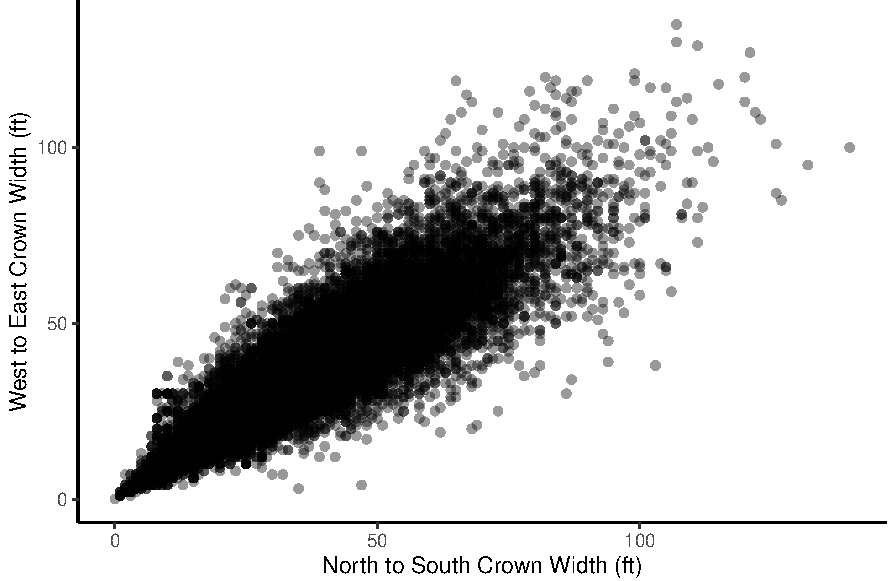
\includegraphics{thesis_files/figure-latex/crownWidth-1} 

}

\caption{Plot comparing North to South Crown Width (ft) to West to East Crown Width (ft). A tree with a higher north-south crown width has a higher west-east crown width, so without loss of generality the north-south crown width variable is used to filter the dataset for larger trees only.}\label{fig:crownWidth}
\end{figure}
Six tree types were determined to have large enough canopies on average and appear frequently enough to construct a training dataset with sufficient observations for each species of tree: Douglas-Fir, English Oak, Giant Sequoia, Maple, Western Redcedar. Table \ref{tab:pointsTable} provides the number of trees under each common name category. The largest group contains 6485 observations of Douglas-Fir trees, and the smallest group contains 135 observations of English Oak trees.
\begin{table}

\caption{\label{tab:pointsTable}Common names of trees included in the data and their total counts.}
\centering
\begin{tabular}[t]{l|r}
\hline
Tree Name & Tree Count\\
\hline
Douglas-Fir & 6485\\
\hline
Norway Maple & 1406\\
\hline
Western Redcedar & 652\\
\hline
Bigleaf Maple & 464\\
\hline
Giant Sequoia & 315\\
\hline
English Oak & 135\\
\hline
\end{tabular}
\end{table}
\hypertarget{creating-spatial-polygons}{%
\subsection{Creating Spatial Polygons}\label{creating-spatial-polygons}}

The training dataset was converted into shapefiles for each type of tree and exported into QGIS where polygons were manually drawn around 100 of the trees for each species. The point shapefile layers were displayed over the raster images downloaded from Planet.com in QGIS, which provided a guide point for locating individual trees. Then using QGIS's drawing tool, a polygon is carefully drawn around the tree canopy (see Figure \ref{fig:polyimage} and Figure \ref{fig:redcedar}). Most polygons turned out to be four to six-sided polygons to retain the general shape of the tree canopy. Tree polygons were only created if the outline of the tree canopy was clearly visible or surrounded by other trees of the same species in order to avoid including pixels from the wrong species in that polygon. Also, the shadows of the trees are visible in the raster images, so the polygons were drawn with the intention of not including the tree shadow. For the five different species of trees, at least 100 polygons were drawn around trees of that type, with each polygon containing at least 6 pixels and at most 20 pixels. The polygon shapefiles were then exported into RStudio where the rest of the analysis was conducted.

Table \ref{tab:polyCounts} displays the number of polygons per raster strip and the amount of pixels from those polygons. Table \ref{tab:polyCountsTrees} displays these counts in terms of tree species.
\begin{figure}

{\centering 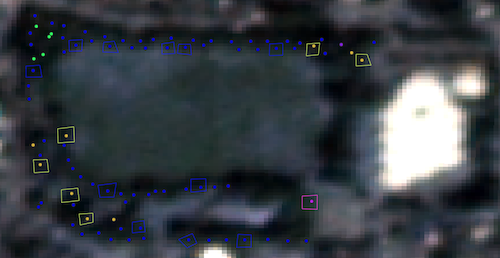
\includegraphics[width=0.5\linewidth]{figure/polyimage} 

}

\caption{Polygons drawn around different tree species: maples (blue), sequoias (yellow), redcedars (pink). Note there are no polygons around trees with canopies that overlap with canopies of different tree species, like douglas-firs (green), to avoid misclassifying pixels from different tree species.}\label{fig:polyimage}
\end{figure}
\begin{figure}

{\centering 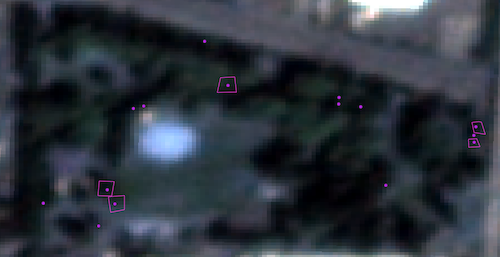
\includegraphics[width=0.5\linewidth]{figure/redcedar} 

}

\caption{Polygons drawn around redcedar trees}\label{fig:redcedar}
\end{figure}
\begin{table}

\caption{\label{tab:polyCounts}Number of polygons per raster strip}
\centering
\begin{tabular}[t]{l|r|r}
\hline
Raster Strip & Polygons & Pixels\\
\hline
a & 197 & 3614\\
\hline
b & 257 & 4887\\
\hline
c & 36 & 359\\
\hline
d & 8 & 98\\
\hline
e & 177 & 2395\\
\hline
\end{tabular}
\end{table}
\begin{table}

\caption{\label{tab:polyCountsTrees}Number of polygons per tree type per raster strip}
\centering
\begin{tabular}[t]{l|l|r|r}
\hline
Raster Strip & Tree Name & Polygons & Pixels\\
\hline
a & Bigleaf Maple & 28 & 283\\
\hline
a & Douglas-Fir & 35 & 432\\
\hline
a & English Oak & 30 & 288\\
\hline
a & Giant Sequoia & 26 & 336\\
\hline
a & grass & 1 & 1158\\
\hline
a & Norway Maple & 48 & 747\\
\hline
a & Western Redcedar & 29 & 370\\
\hline
b & Bigleaf Maple & 26 & 279\\
\hline
b & Douglas-Fir & 38 & 604\\
\hline
b & English Oak & 62 & 618\\
\hline
b & Giant Sequoia & 32 & 399\\
\hline
b & grass & 3 & 1579\\
\hline
b & Norway Maple & 70 & 1026\\
\hline
b & Western Redcedar & 26 & 382\\
\hline
c & Bigleaf Maple & 9 & 55\\
\hline
c & Douglas-Fir & 19 & 202\\
\hline
c & English Oak & 2 & 39\\
\hline
c & Western Redcedar & 6 & 63\\
\hline
d & Douglas-Fir & 5 & 56\\
\hline
d & Western Redcedar & 3 & 42\\
\hline
e & Bigleaf Maple & 37 & 268\\
\hline
e & Douglas-Fir & 6 & 86\\
\hline
e & English Oak & 6 & 80\\
\hline
e & Giant Sequoia & 54 & 701\\
\hline
e & grass & 1 & 186\\
\hline
e & Norway Maple & 37 & 567\\
\hline
e & Western Redcedar & 36 & 507\\
\hline
\end{tabular}
\end{table}
\hypertarget{polygon-limitations}{%
\subsection{Polygon Limitations}\label{polygon-limitations}}

Ideally, the raster strips contain training trees of each species, and as a result, the polygons are evenly distributed across the raster strips, but due to limitations of our ground-level data as well as the coverage of the strips across the city of Portland, this is not achievable. Each of the raster strips contains some number of manually drawn polygons, however, raster strips `C' and `D' are missing some of the tree species. The raster strips do not all cover Portland to the same extent. Strips `A' and `B' encompass most of the city while strips `C' and `D' only make up a small portion that covers the corners of the city not reached by strips `A' and `B'.

The polygons are drawn with the intention of locating and extracting pixels for a known tree species. Ideally, the extracted data is representative of tree pixels and has a sufficient amount of pixels per species. The satellite images' resolution makes some error inevitable. If tree canopies overlap, polygons may contain pixels from different species. If pixels are cast in shadow, the extracted light intensity values will differ from other pixel values. To avoid these errors, polygons with uncertain canopies are cross-checked with the satellite filter on Google Maps. For example, a point in QGIS that is indicated as a douglas-fir tree might appear as one tree on the low-resolution image from Planet.com, but a closer look at Google Maps shows that it is actually two trees in close proximity. Having low spatial resolution decreases the number of pixels available within a polygon, but that has to be balanced out with the need for a large number of pixels. With regards to the number of pixels per tree species, having around the same number of tree polygons per species results in differing amounts of pixels per species due to the different average sizes of tree canopies for different species. After drawing the images, the pixels totals per tree species is computed to ensure that the training pixels data contains at least 800 pixels per tree species.

\hypertarget{combining-ground-level-data-with-pixel-level-data}{%
\subsection{Combining Ground-level Data with Pixel-level Data}\label{combining-ground-level-data-with-pixel-level-data}}

The first spatial join in RStudio was conducted to match up each Spatial Polygon with a point in the training dataset. Then the raster images were loaded and joined with the polygons to extract the pixel values inside each polygon for all 4 bands (red, green, blue, infrared). Ultimately this turned into a pixel table with rows representing each pixel with its corresponding polygon, light reflection intensity values for all 4 bands, and the ground information about that tree. Table \ref{tab:pixelHead} displays the first few entries of the pixels dataset. Table \ref{tab:pixelCounts} contains the summary of the total number of pixels for each tree type.
\begin{table}

\caption{\label{tab:pixelHead}Variables and pixel values included in the pixels dataset}
\centering
\resizebox{\linewidth}{!}{
\begin{tabular}[t]{r|r|r|r|r|l|l|l|l|l|r|r|r|l|l|r|r|r|r|r}
\hline
ID & red & green & blue & ir & rstrip & id\_type & Genus & Species & Cmmn\_Nm & Cr\_W\_NS & Cr\_W\_EW & Crw\_B\_H & Conditn & St\_Wdth & ndvi & red\_blue & ir\_red & red\_green & blue\_green\\
\hline
43 & 4707 & 4125 & 3187 & 6627 & a & acpl & Acer & ACPL & Norway Maple & 28 & 28 & 8 & Fair & NA & 0.1694018 & 1.476938 & 1.407903 & 1.141091 & 0.7726061\\
\hline
43 & 4384 & 3860 & 2864 & 7111 & a & acpl & Acer & ACPL & Norway Maple & 28 & 28 & 8 & Fair & NA & 0.2372336 & 1.530726 & 1.622035 & 1.135751 & 0.7419689\\
\hline
43 & 4446 & 3803 & 2807 & 7443 & a & acpl & Acer & ACPL & Norway Maple & 28 & 28 & 8 & Fair & NA & 0.2520818 & 1.583897 & 1.674089 & 1.169077 & 0.7381015\\
\hline
43 & 4619 & 3911 & 2859 & 7801 & a & acpl & Acer & ACPL & Norway Maple & 28 & 28 & 8 & Fair & NA & 0.2561997 & 1.615600 & 1.688894 & 1.181028 & 0.7310151\\
\hline
43 & 4695 & 4060 & 3201 & 5996 & a & acpl & Acer & ACPL & Norway Maple & 28 & 28 & 8 & Fair & NA & 0.1216911 & 1.466729 & 1.277103 & 1.156404 & 0.7884236\\
\hline
43 & 4344 & 3719 & 2728 & 6747 & a & acpl & Acer & ACPL & Norway Maple & 28 & 28 & 8 & Fair & NA & 0.2166622 & 1.592375 & 1.553177 & 1.168056 & 0.7335305\\
\hline
\end{tabular}}
\end{table}
\begin{table}

\caption{\label{tab:pixelCounts}Number of pixels per tree type}
\centering
\begin{tabular}[t]{l|r}
\hline
Tree Name & Pixels Count\\
\hline
Bigleaf Maple & 885\\
\hline
Douglas-Fir & 1380\\
\hline
English Oak & 1025\\
\hline
Giant Sequoia & 1436\\
\hline
grass & 2923\\
\hline
Norway Maple & 2340\\
\hline
Western Redcedar & 1364\\
\hline
\end{tabular}
\end{table}
Figure \ref{fig:pixDensity} displays the range of reflection intensity pixel values per tree type. Each tree species has similar ranges of values over the red, green, blue, and infared bands. Of the species included in the training data, the grass bands appear to differ the most in terms of its infrared density.
\begin{figure}

{\centering 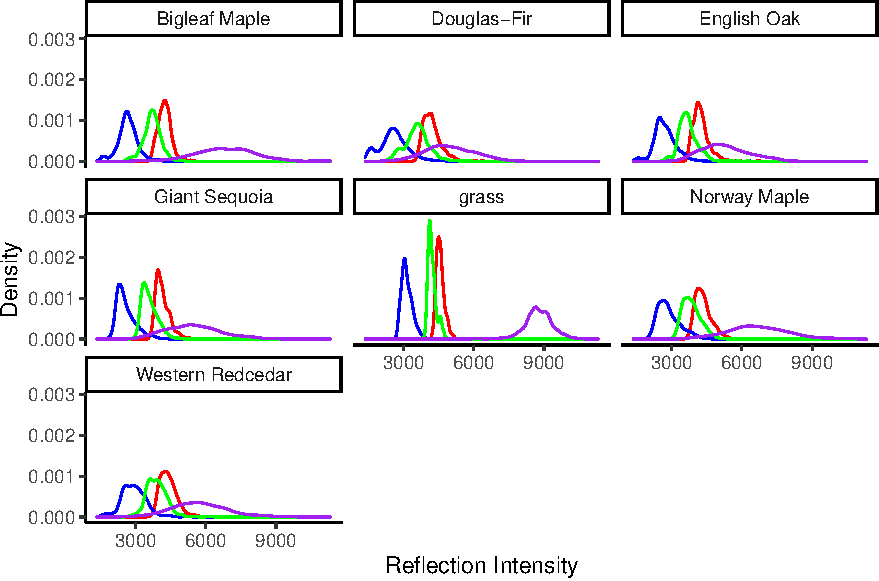
\includegraphics{thesis_files/figure-latex/pixDensity-1} 

}

\caption{Range of reflection intensity pixel values per tree type.}\label{fig:pixDensity}
\end{figure}
\hypertarget{preparing-raster-images}{%
\chapter{Preparing Raster Images}\label{preparing-raster-images}}

The training model has to be applied to the entire raster image to predict the location of Western Redcedars, however, extracting all the pixels from raster images is a slow process. Filtering the rasters to keep vegetation and to recognize the difference between grass pixels and tree pixels alleviates the computational intensity of extracting all the pixels and improves the performance of the models. To reduce the size of computations, all five raster strips are masked and cropped to only include pixels within the city boundary of Portland, since that is the region of interest, and that is the extent of the ground level data.

\hypertarget{masking-vegetation}{%
\section{Masking Vegetation}\label{masking-vegetation}}

The satellite images in RStudio need to be masked to reduce the number of pixels that the model has to classify and prevent the chance of a non-vegetation surface being predicted as a tree. A common mask applied to raster images is a Normalized Difference Vegetation Index (NDVI) mask. This index is a measure of the greenness of a pixel, with higher values indicating vegetation and lower values indicating infertile areas such as a rock. The formula for NDVI is \(NDVI = \frac{NIR - Red}{NIR + Red}\). Figure \ref{fig:ndvival} displays the density of NDVI values over the raster images. To remove the pixels that are not vegetation, an NDVI threshold is determined to be 0.00 to create a mask dividing the pixels into vegetation (1) and non-vegetation (0). When the trained model is applied to the raster image, it is applied to the masked raster image that only keeps pixels with NDVI mask values of 1.
\begin{figure}

{\centering 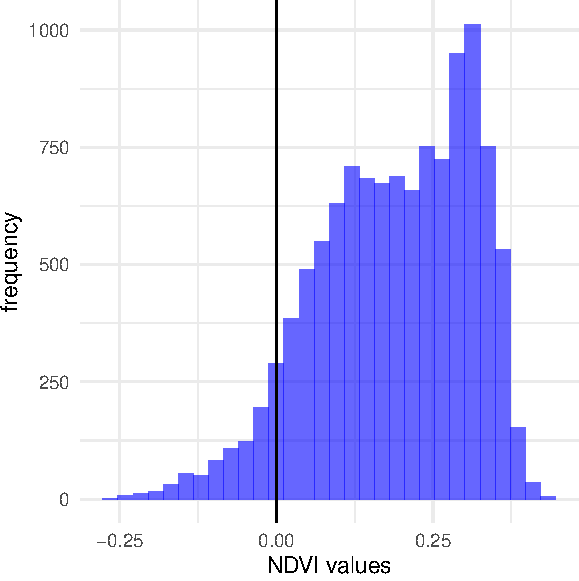
\includegraphics{thesis_files/figure-latex/ndvival-1} 

}

\caption{Normalized Difference Vegetation Index (NDVI) is a measure of the greenness of a pixel. The histogram displays the frequency of the tree pixels' NDVI values. A good threshold for masking out the nonvegetation pixels is an NDVI of 0.}\label{fig:ndvival}
\end{figure}
\hypertarget{masking-grass}{%
\section{Masking Grass}\label{masking-grass}}

After masking the images to only contain vegetation pixels, the effectiveness of a second mask was investigated to try and determine whether it is feasible to distinguish between tree pixels and grass pixels in a satellite image. This would be useful for preventing the final model from predicting fields of grass as trees. Inspired by previous research, a grass index was created by averaging the values of the four bands, \(GRASS = \frac{RED + BLUE + GREEN + NIR}{4}\) (Qian, Zhou, Nytch, Han, \& Li, 2020). Grass polygons were created in QGIS to add a grass attribute in the pixels dataset. Five fields of grass were outlined as polygons in QGIS. In RStudio, the pixels were extracted from the grass polygons for a total of 2,923 grass pixels. Figure \ref{fig:grassval} displays how the average band values for the grass pixels differ from the other tree types average band values. Based on the figure, pixels in the raster image that have an average band value above 4900 are filtered out. Masking the grass pixels ensures that a field of grass will not be classified as a tree when applied to the entire raster image.
\begin{figure}

{\centering 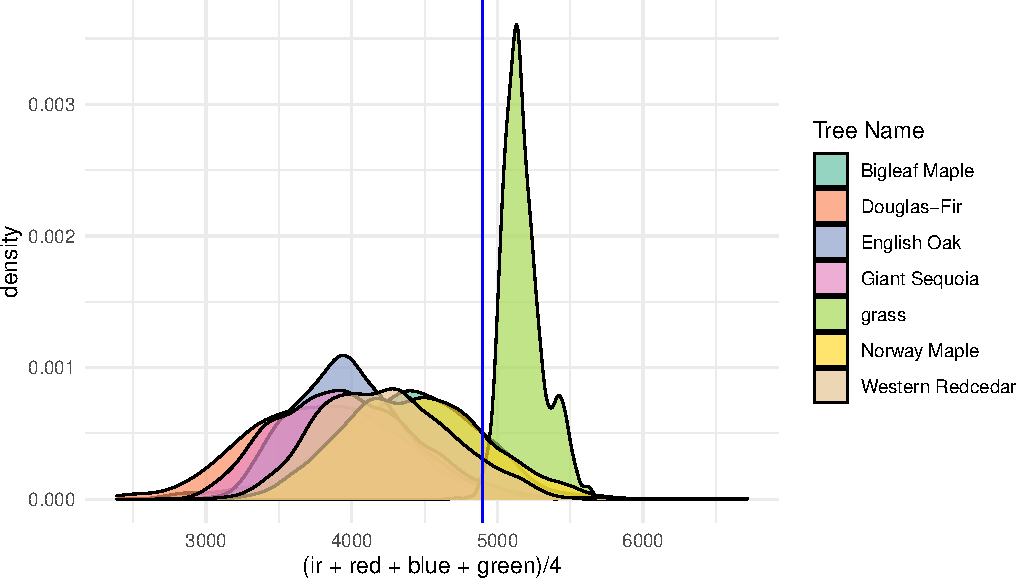
\includegraphics{thesis_files/figure-latex/grassval-1} 

}

\caption{Average of band values distribution across different tree types in comparison with grass pixel average band values. Most grass pixels have an average value above 4900, so a mask is applied to the raster image to remove pixels with average values above this threshold.}\label{fig:grassval}
\end{figure}
Figure \ref{fig:beforeaftermask} displays a raster strip with every pixel included (top), only the pixels with NDVI values above 0.00 (middle), and only pixels with NDVI values above 0.00 and average band values below 4900 (bottom). Ideally, the bottom image is left with only the tree pixels in the image.
\begin{figure}

{\centering 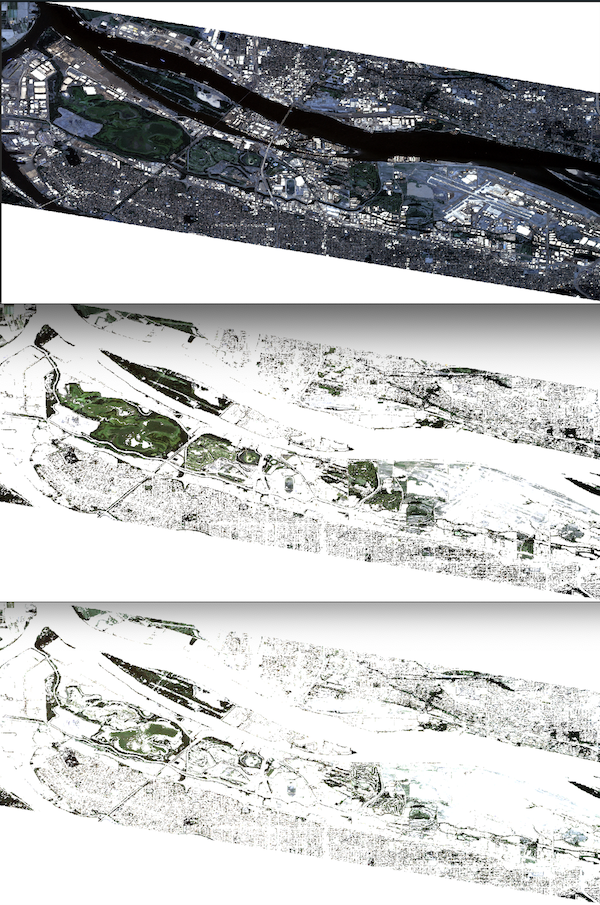
\includegraphics[width=0.4\linewidth]{figure/beforeaftermask} 

}

\caption{A raster strip with every pixel included (top), only the pixels with NDVI values above 0.00 (middle), and only pixels with NDVI values above 0.00 and average band values below 4900 (bottom)}\label{fig:beforeaftermask}
\end{figure}
\hypertarget{masking-limitations}{%
\section{Masking Limitations}\label{masking-limitations}}

The low resolution of the raster images cause shapes to appear blurry, and especially tree canopies that are close together appear as a single formation.

Masked raster images were imported in QGIS and compared to Google Maps. In general, the NDVI mask was successful in keeping the forest pixels while still removing building structures and roads. For the GRASS mask, if a field of grass is a brownish color, it gets removed, but some greener fields are not masked out. The masks consistently remove river pixels but not lake pixels if the lake is a greenish color. For example, Smith Lake in North Portland is considered an urban wetland, which signifies a body of water with a lot of vegetation. From the perspective of a satellite, this region has NDVI values consistent with vegetation. However, the average band pixel values are less than 4900, so they are not masked out by the final GRASS mask stage, and instead are treated as tree pixels in the model (see Figure \ref{fig:masklimit}).

To address leftover grass pixels in the filtered raster image, access to lidar data would provide a method of determining the height of certain pixels. Setting a height threshold would ensure that grass pixels are removed while higher vegetation pixels are kept. This would also address the masks' limitations in removing lakes with high vegetation, since those pixels would not meet the threshold for height. The GRASS mask did not perform as hoped, so the grass pixels extracted from polygons were included to train the model to distinguish observations as trees or grass pixels instead of applying a second mask on the raster images.
\begin{figure}

{\centering 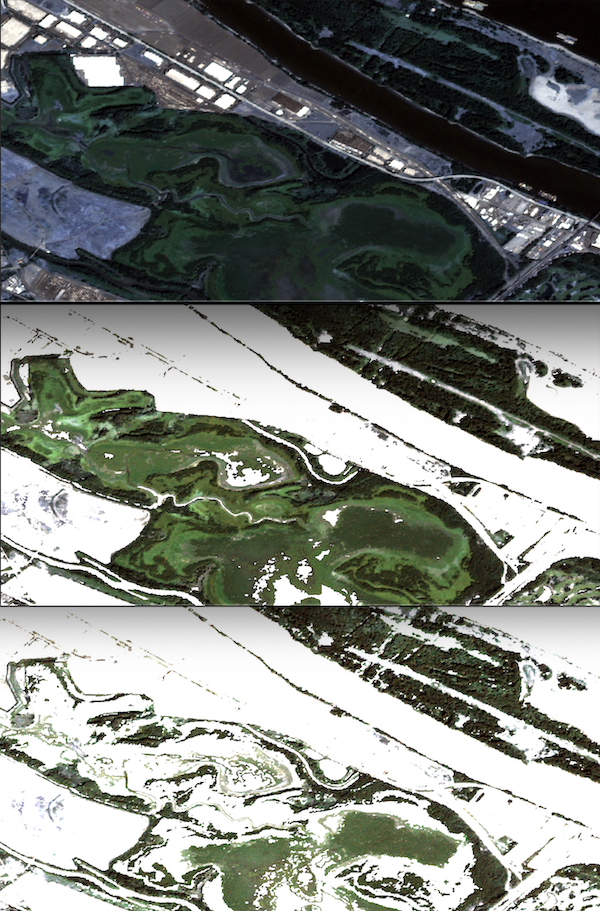
\includegraphics[width=0.4\linewidth]{figure/masklimit} 

}

\caption{Satellite view of Smith Lake (top), after NDVI mask applied (middle), and NDVI mask and GRASS mask applied (bottom). The final masked image still contains parts of the lake because the aquatic vegetation fits the pixel values descriptions set by the masks.}\label{fig:masklimit}
\end{figure}
\hypertarget{methods}{%
\chapter{Methods}\label{methods}}

\hypertarget{existing-methods}{%
\section{Existing Methods}\label{existing-methods}}

Since the Western Redcedar decline is recent, there are currently no published work for identifying tree species like Western Redcedars for the Pacific Northwest using satellite imaging. One literature investigates the dieback of Wester redcedars in Vancouver, B.C. as a result of dry weather and how this links to climate change (Seebacher, 2007). A study identifies tree species for a strip of land in California by combining ground-level data with satellite images (Fricker et al., 2019). Their methods involved drawing polygons around rastered images that are layered with ground data as explained in Chapter \ref{data}, but the pixels from the polygons are used to train a convolutional neural network (CNN) model instead of the random forests and support vector machines in this study. The CNN model was then evaluated with k-fold cross validation. CNN models are appropriate in a classification setting and when working with satellite images because they account for spatial relations, which is likely to appear in classifying tree species. This study follows the methods of preparing the data for modelling as well as the method of cross validation to evaluate the performance of the random forests and support vector machines models. Random forests are used in a classification setting or regression setting and have the advantage of being simplier to train than CNN models and still performs at a similar level. Random forests apply an element of randomness to create a lot of decision trees and improve the classification power. Since this research strives to provide a computationally simple method of estimating tree locations to track changes in the ecosystem, a random forest is suitable for the study. If a researcher was interested in making more precise predictions, a CNN would require more time but would produce better estimates.

\hypertarget{current-methods}{%
\section{Current Methods}\label{current-methods}}

This research applies RF and SVM models on trained data and compares overall training performance, overall testing performance, overall polygon testing accuracy, and Western Redcedar training and testing performance. The following sections provide background about RF and SVM models.

\hypertarget{random-forest}{%
\subsection{Random Forest}\label{random-forest}}

In building a decision tree (Figure \ref{fig:decisiontree}) for classification, recursive binary splits are made by minimizing the Gini index (\(G\)), the total variance across \(K\) classes:

\[G = \sum_{k = 1}^K\hat{p}_{mk}(1 - \hat{p}_{mk}),\]

where \(\hat{p}_{mk}\) is the proportion of observations in the \(m^{\text{th}}\) region from the \(k^{\text{th}}\) class (James, Witten, Hastie, \& Tibshirani, 2013).
\begin{figure}

{\centering 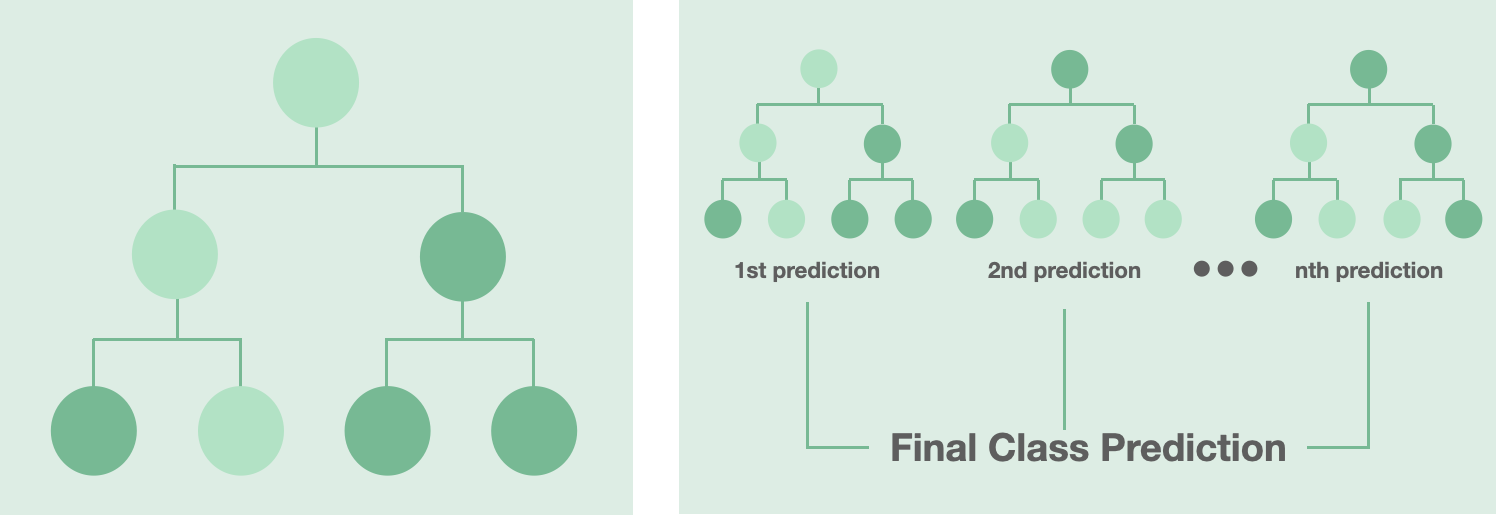
\includegraphics[width=0.7\linewidth]{figure/decision_tree} 

}

\caption{A single decision tree (left) displays splits at different predictors. Random forests (right) are constructed by aggregating many decision trees constructed from bootstrapped samples of the data and from splits made from a random subset of predictors.}\label{fig:decisiontree}
\end{figure}
A small Gini index value represents a region containing mostly observations from a single class, while a large Gini index value represents a lot of variation across classes. Then the decision tree is constructed by repeatedly considering different attributes and making splits where the Gini index is minimized. This is a ``top-down, greedy'' approach in the sense that, at the first stage, the optimal decision is made, and again, at the next stage, the optimal decision is made, and so on. Note that this top-down, greedy approach tends to overfit the training data, so finding the decision tree that performs the best on test data involves a cost-complexity pruning algorithm to obtain smaller trees and apply k-fold cross validation to choose the best tree that minimizes the average error. Instead of pruning the tree to deal with overfitting, another option is aggregating bootstrapped decision trees constructed with a random element through considering random subsets of the predictors. K-fold cross validation is performed when training the models by splitting the data into \(k = 10\) folds and training ten models each time withholding one of the ten folds to evaluate the accuracy of the model against the remaining nine folds and repeating the process until each fold is left out. This process aids in understanding how the models will perform against data that has not been included in training the model. Larger decision trees are more sensitive to changes in the training data, and so, have higher variance.

In the classification setting, a stronger predictive model than a decision tree is a random forest (Figure \ref{fig:decisiontree}), which involves the construction of many bootstrapped decision trees. The simple method of sampling with replacement from the data and forming decision trees on the boostrapped samples ends up producing many similar, correlated trees. Random forests apply an element of randomness to decorrelate bootstrapped decision trees. Bootstrapped samples from the training dataset are used to construct decision trees, where splits are based on minimizing the Gini index when selecting from a random sample \(m\) of attributes from all \(p\) available. In common random forest applications, the number of attributes considered at a split is \(m \approx \sqrt{p}\). Theoretically, by forcing only a subset of attributes to be featured in the tree, this expands the number of possible subtrees that might not have been achieved by the top-down, greedy approach. Hence, random forests provide a method of predicting classes with low variance while also keeping bias at a minimum.

\hypertarget{support-vector-machine}{%
\subsection{Support Vector Machine}\label{support-vector-machine}}

Another method investigated in this study imagines the multidimensional data in space and classifies the data using hyperplanes positioned to minimize misclassification error and maximize distance from observations to separate the data (James et al., 2013). The maximal margin hyperplane is a plane that separates data so that one class is on one side and another class is on the other side. Figure \ref{fig:hyperplane} displays a two dimensional example where a line separates two classes. Depending on the data, there could be many ways of drawing this line or zero ways. Since test data observations might be positioned close to the hyperplane, the optimal classifier is the hyperplane that maximizes the perpendicular distance between observations and the plane while keeping the classes separated. Observations that are closer to the hyperplane are called support vectors because they have more influence over the line if they move than observations that are further. Observations which are further from the hyperplane than support vectors do not have as much influence because a small movement in those observations does not impact the location of the hyperplane. A large number of support vectors indicates the classifier has low variance and high bias.
\begin{figure}

{\centering 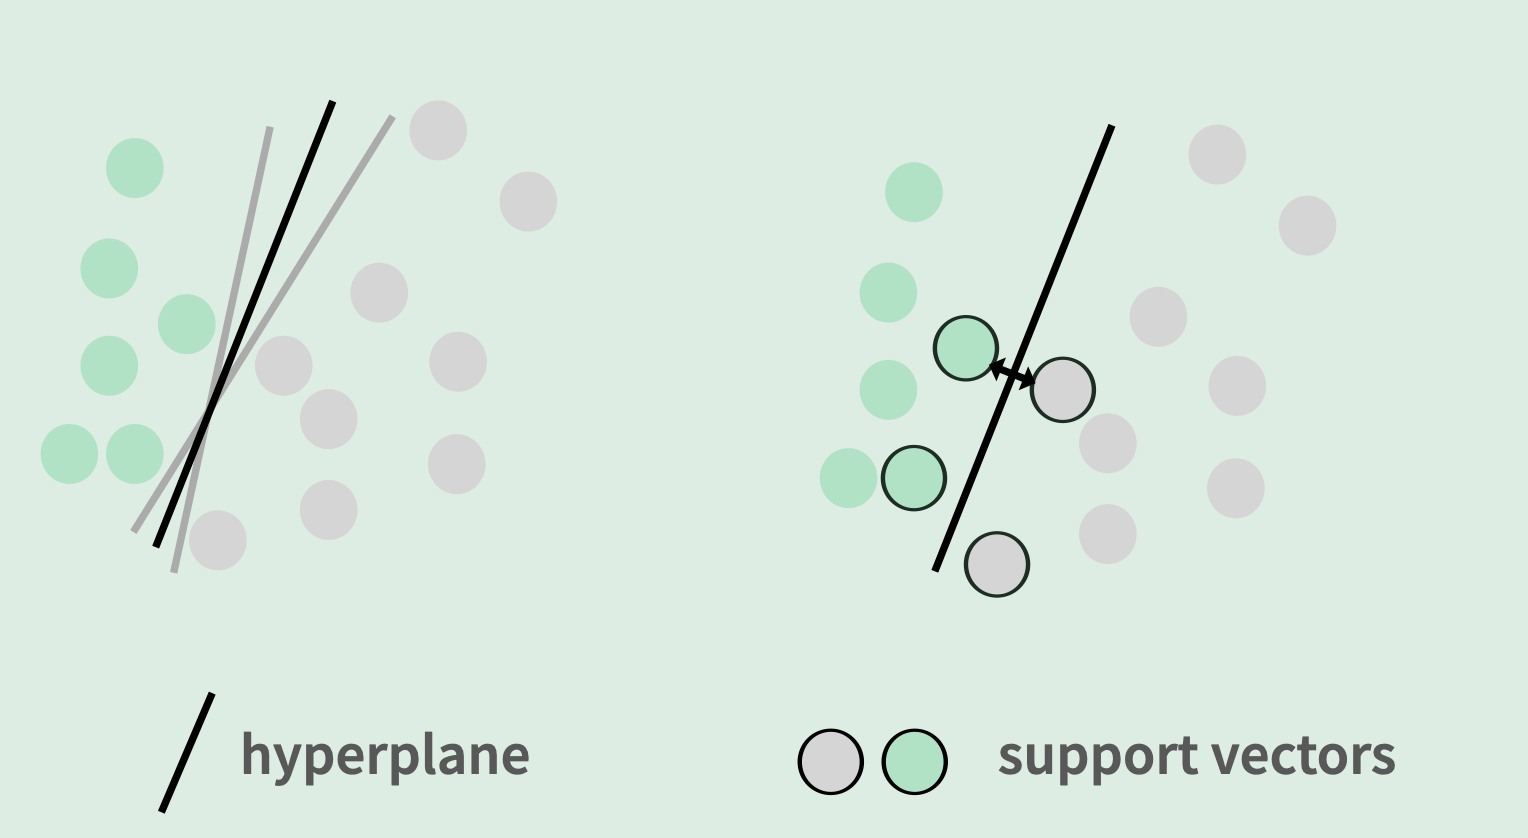
\includegraphics[width=0.7\linewidth]{figure/hyperplane} 

}

\caption{Left: Depending on the data, there could be several ways of drawing a hyperplane or zero ways. If it is possible to separate the classes, the plane that maximizes the perpendicular distance between observations and the plane is the optimal classifier. Right: Points that are close to the hyperplane are support vectors in the sense that slight changes in these points will alter the hyperplane.}\label{fig:hyperplane}
\end{figure}
More specifically, the following algorithm is applied to determine the maximal margin hyperplane for observations \(x_1, ..., x_n \in \mathbb{R}^p\) with classes \(y_1, ..., y_n \in \{-1, 1\}\) and \(p\) predictors:
\begin{enumerate}
\def\labelenumi{(\arabic{enumi})}
\item
  Choose \(\beta_0, \beta_1, ..., \beta_p\) to maximize margin of hyperplane (M)
\item
  Apply constraints to ensure that observations are M away from the hyperplane and on the correct side:
  \[\sum_{j = 1}^p \beta_j^2 = 1 \text{ and } y_i(\beta_0 + \beta_1 x_{i1} + \beta_2 x_{i2} + ... + \beta_p x_{ip}) \geq M \  \forall \ i = 1, ..., n.\]
\end{enumerate}
This determines the optimal hyperplane separating the data if it exists, however, there are some cases where the data cannot be perfectly separated by a plane, which is where suppor vector machines are appropriate.

The support vector classifier allows some observations to be misclassified with some meaure of error \(\epsilon_i\). This \(\epsilon_i\) is 0 if the observation is on the correct side of the margin, between 1 and 0 if the observation is on the wrong side of the margin, and greater than \(1\) if it is on the wrong side of the hyperplane. A tuning parameter \(C\) is the cost measure for the amount of error we are willing to allow. Higher values of \(C\) are more tolerant of misclassifications, so the margin is wider.

The following algorithm determines the support vector classifier for observations \(x_1, ..., x_n \in \mathbb{R}^p\) with classes \(y_1, ..., y_n \in \{-1, 1\}\) and \(p\) predictors:
\begin{enumerate}
\def\labelenumi{(\arabic{enumi})}
\item
  Choose \(\beta_0, \beta_1, ..., \beta_p, \epsilon_1, ..., \epsilon_n\) to maximize margin of hyperplane (M)
\item
  Apply constraints to ensure that observations are M away from the hyperplane and on the correct side:
\end{enumerate}
\[\sum_{j = 1}^p \beta_j^2 = 1, \  y_i(\beta_0 + \beta_1 x_{i1} + \beta_2 x_{i2} + ... + \beta_p x_{ip}) \geq M(1 - \epsilon_i) \  \forall \ i = 1, ..., n, \ \epsilon_i \geq 0, \ \sum_{i = 1}\epsilon_i \leq C.\]

Support vector machines take the concept of support vector classifiers and extend the feature space while also making computations efficient to account for nonlinear boundaries using kernels. The three kernels explored in this study were the linear, radial, and polynomial kernel. The diagrams in Figure \ref{fig:diagrams} display how different kernels are more appropriate depending on the structure of the data and the relationship between classes.
\begin{figure}

{\centering 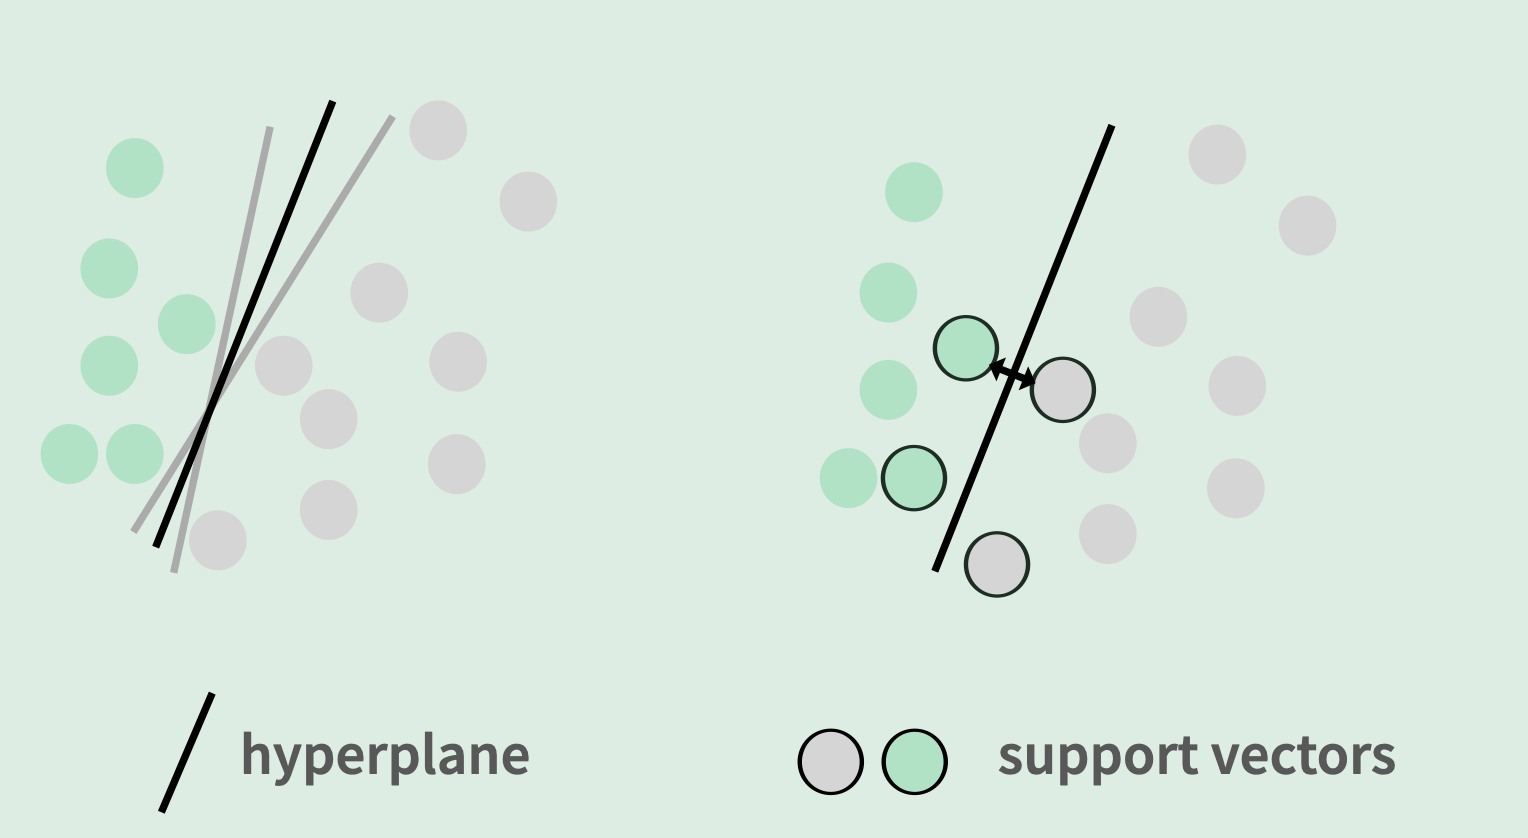
\includegraphics[width=0.7\linewidth]{figure/hyperplane} 

}

\caption{Left: The linear kernel creates a linear boundary between two classes. Middle: The radial kernel successful models data where one class is surrounded by the other class. Right: The polynomial kernel is slightly more flexible than the linear kernel.}\label{fig:diagrams}
\end{figure}
Each kernel has its own set of cost parameters to tune with cross validation.

A linear kernel is

\[K(x_i, x_{i'}) = \sum_{j = 1}^p x_{ij}x_{i'j}\]
with a support vector classifier

\[f(x) = \beta_0 + \sum_{i = 1}^n \alpha_i \langle x, x_i \rangle.\]

The parameters \(\alpha_i\) and \(\beta_0\) are estimated using the inner products of the observations, but \(\alpha_i \neq 0\) if and only if \(x_i\) is a support vector. Note that this function is similar to a linear regression function, and the kernel function is the correlation between pairs of points. Extending this model to a nonlinear context involves a similar approach as adding nonlinear terms to a regression model.

The polynomial kernel of degree \(d\) is defined to be

\[K(x_i, x_{i'}) = \left( 1 + \sum_{j = 1}^p x_{ij}x_{i'j}\right)^d\]

with support vector classifier

\[f(x) = \beta_0 + \sum_{i = 1}^n \alpha_i K(x, x_i).\]
For some positive constant \(k\), the radial kernel is defined to be

\[K(x_i, x_{i'}) = \mbox{exp}\left( -\gamma\sum_{j = 1}^p(x_{ij} - x_{i'j})^2 \right),\]

which applies constraints so that the model is more sensitive to nearby observations as opposed to further observations.

The cost parameters of support vector machines can be altered to construct models that are less sensitive to outliers and ultimately become successful predictors of categorical variables in high-dimensional data. A support vector machine does not perform well for data with observations that overlap and if the kernel is incorrectly selected.

\hypertarget{training-models}{%
\section{Training Models}\label{training-models}}

Data used to train the RF and SVM models are the pixels training data and the point pixels training data. To prepare the data for modelling, first the data is separated into a training set and then a test set by a ratio of 70\% training data and 30\% testing data. The \texttt{dplyr} function \texttt{slice\_sample} was used to take a stratified sample from the entire pixels dataset where 70\% of each tree species in an individual raster strip was randomly selected. For example, the training set consisted of 70\% of the bigleaf maple trees in raster strip `A', 70\% of bigleaf maple trees in raster strip `B', and so on. From the 70\% pixels training data, 500 observations for each tree species are randomly extracted to obtain an even distribution of species. From the point pixels training data, 190 observations for each tree species are sampled.

The selected variables for training the models are the four bands (red, green, blue, infrared) and an NDVI variable, and the predictive variable is the tree species name. Some predictor variables were manually computed using ratios of bands. Typically, a long over short band ratio provides some more information to train the model. The following bands were created: red/blue, ir/red, red/green, and blue/green. Examining a correlation matrix with these predictors reveals possibly informative and not too highly correlated variables are red/green, red/blue, and blue/green (see Figure \ref{fig:corrmatrix}).
\begin{figure}

{\centering 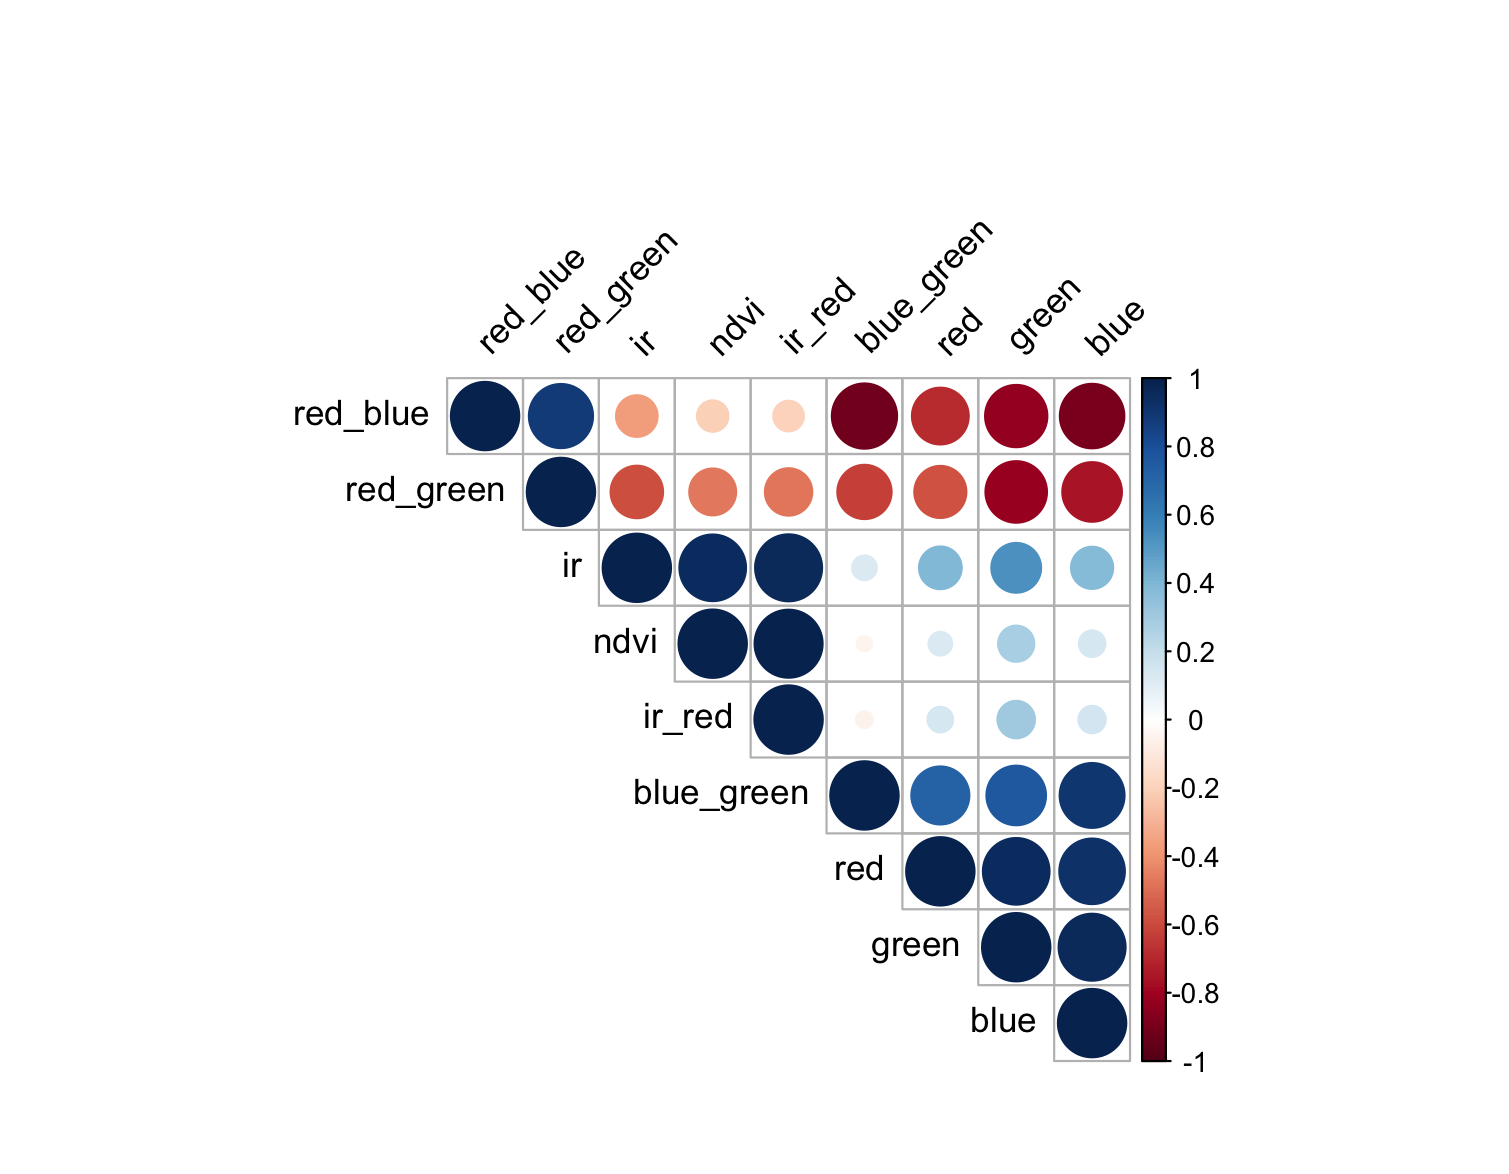
\includegraphics[width=0.7\linewidth]{figure/corrmatrix} 

}

\caption{Correlation matrix of possible predictor variables to include in the model. Size and shade intensity represents stronger correlation (red/blue and blue are highly negatively correlated, while NDVI and green have almost no correlation). Positive correlation indicates higher values of one variable results in higher values of the other variable, while negative correlation indicates higher values of one variable results in lower values of the other variable.}\label{fig:corrmatrix}
\end{figure}
To address the small number of predictor variables available to predict the large number of classes (7 tree species), some species are grouped together. The Bigleaf Maple, Norway Maple, and English Oak species are grouped under a new ``Broadleaf'' tree category. This reduces the number of classes to 5: Broadleaf, Douglas-Fir, Giant Sequoia, Grass, and Western Redcedar. Both the full 7 tree species training data and the grouped (5 class) species training data are used to train the models.

The \texttt{caret} package (Kuhn, 2020) in RStudio provides the framework for the modelling performed in this work. It stands for classification and regression training, and it contains functions for facilitating the process of creating training models in R and determining the tuning parameters.

\hypertarget{random-forest-tuning}{%
\subsection{Random Forest Tuning}\label{random-forest-tuning}}

The \texttt{train} function from the \texttt{caret} package (Kuhn, 2020) with the specified \texttt{method\ =\ rf} option is used to train a random forest model on the training dataset to predict the tree species. The function takes parameters for data, the predictive variable, and the method of training the model. To perform 10-fold cross validation, the \texttt{trainControl} function is used to create an object that tells the \texttt{train} function to perform cross validation 10 times with a different fold left out each time. The function automatically tries multiple number of tries at each split (mtry) and determines the optimal number through cross-validation. Models were considered with total predictors around 7 or 8 predicting classes of size 7 (individual species) or 5 (oaks and maples grouped together):
\begin{itemize}
\item
  7 predictor model: red, green, blue, infrared, NDVI, \(\frac{\mbox{red}}{\mbox{green}}\), \(\frac{\mbox{blue}}{\mbox{green}}\)
\item
  8 predictor model: red, green, blue, infrared, NDVI, \(\frac{\mbox{red}}{\mbox{green}}\), \(\frac{\mbox{red}}{\mbox{blue}}\), \(\frac{\mbox{blue}}{\mbox{green}}\)
\end{itemize}
\hypertarget{predictor-random-forest}{%
\subsubsection{7 predictor Random Forest}\label{predictor-random-forest}}

The 7 predictor random forest model uses the following predictors: red, green, blue, infrared, NDVI, \(\frac{\mbox{red}}{\mbox{green}}\) and \(\frac{\mbox{blue}}{\mbox{green}}\) band values predictors. Figure \ref{fig:rf7} displays the accuracy of the model predicting all 7 tree classes and the grouped 5 classes with the pixels training set with a range of mtry values. The 7 predictor model with the highest accuracy (determined by cross-validation) randomly selected 6 predictors at each split with an accuracy of 0.44. The variable with the highest predictive power was infrared band values with NDVI values with the second highest predictive power. For the grouped data, the optimal mtry value of 1 produced an accuracy of 0.57. The most important variable for this model was infrared followed by NDVI values.
\begin{figure}

{\centering 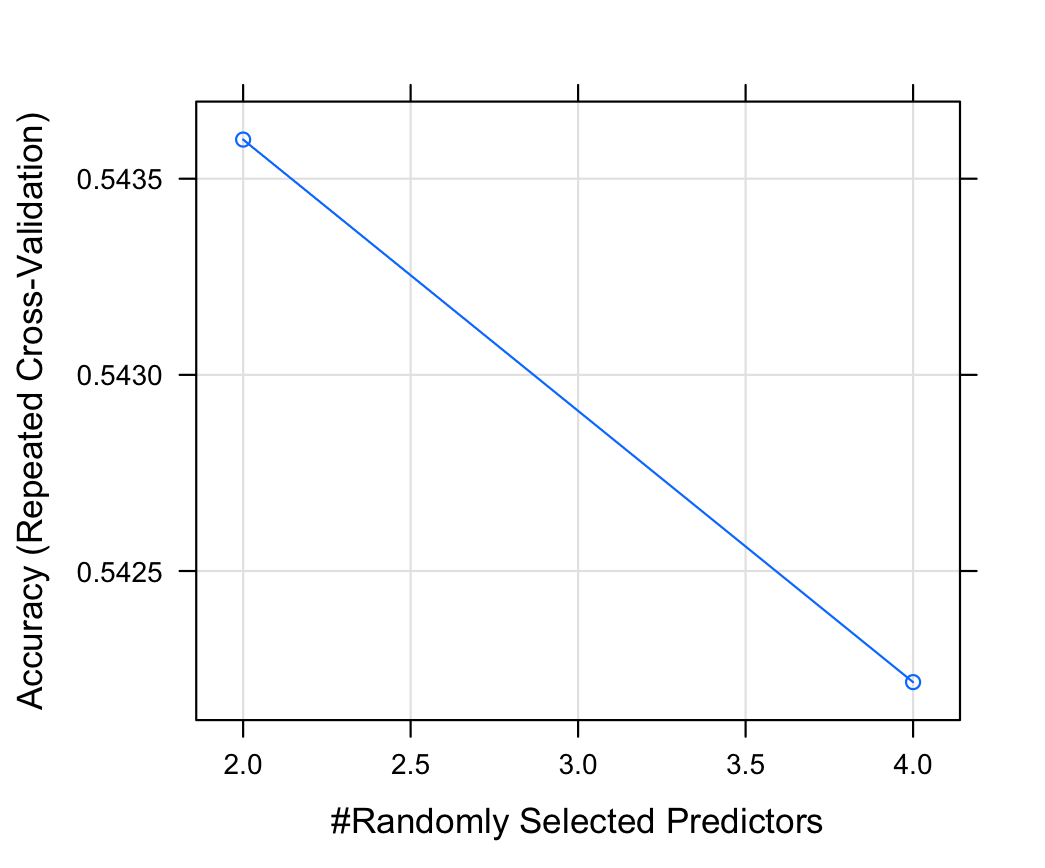
\includegraphics[width=0.9\linewidth]{figure/rf7_mtry} 

}

\caption{Accuracy of the 7 predictor trained random forest model for different mtry numbers over 10-fold cross-validation on 7 class and 5 class training data. (P = Predictors, C = Classes)}\label{fig:rf7}
\end{figure}
\hypertarget{predictor-random-forest-1}{%
\subsubsection{8 predictor Random Forest}\label{predictor-random-forest-1}}

The 8 predictor random forest model added a \(\frac{\mbox{blue}}{\mbox{green}}\) predictor to the 7 predictor model. Figure \ref{fig:rf8} displays the results of a different number of randomly selected predictors to be considered at each split in the tree for 7 class data and 5 class. For modelling all 7 classes, the optimal mtry value was 4 with an accuracy of 0.45. The variables with the higher predictive power in decreasing order were infrared, NDVI, and \(\frac{\mbox{red}}{\mbox{green}}\) band values predictors. The model using grouped data with 5 tree classes, had an optimal mtry value of 8 with an accuracy of 0.57. The most important variable was infrared.
\begin{figure}

{\centering 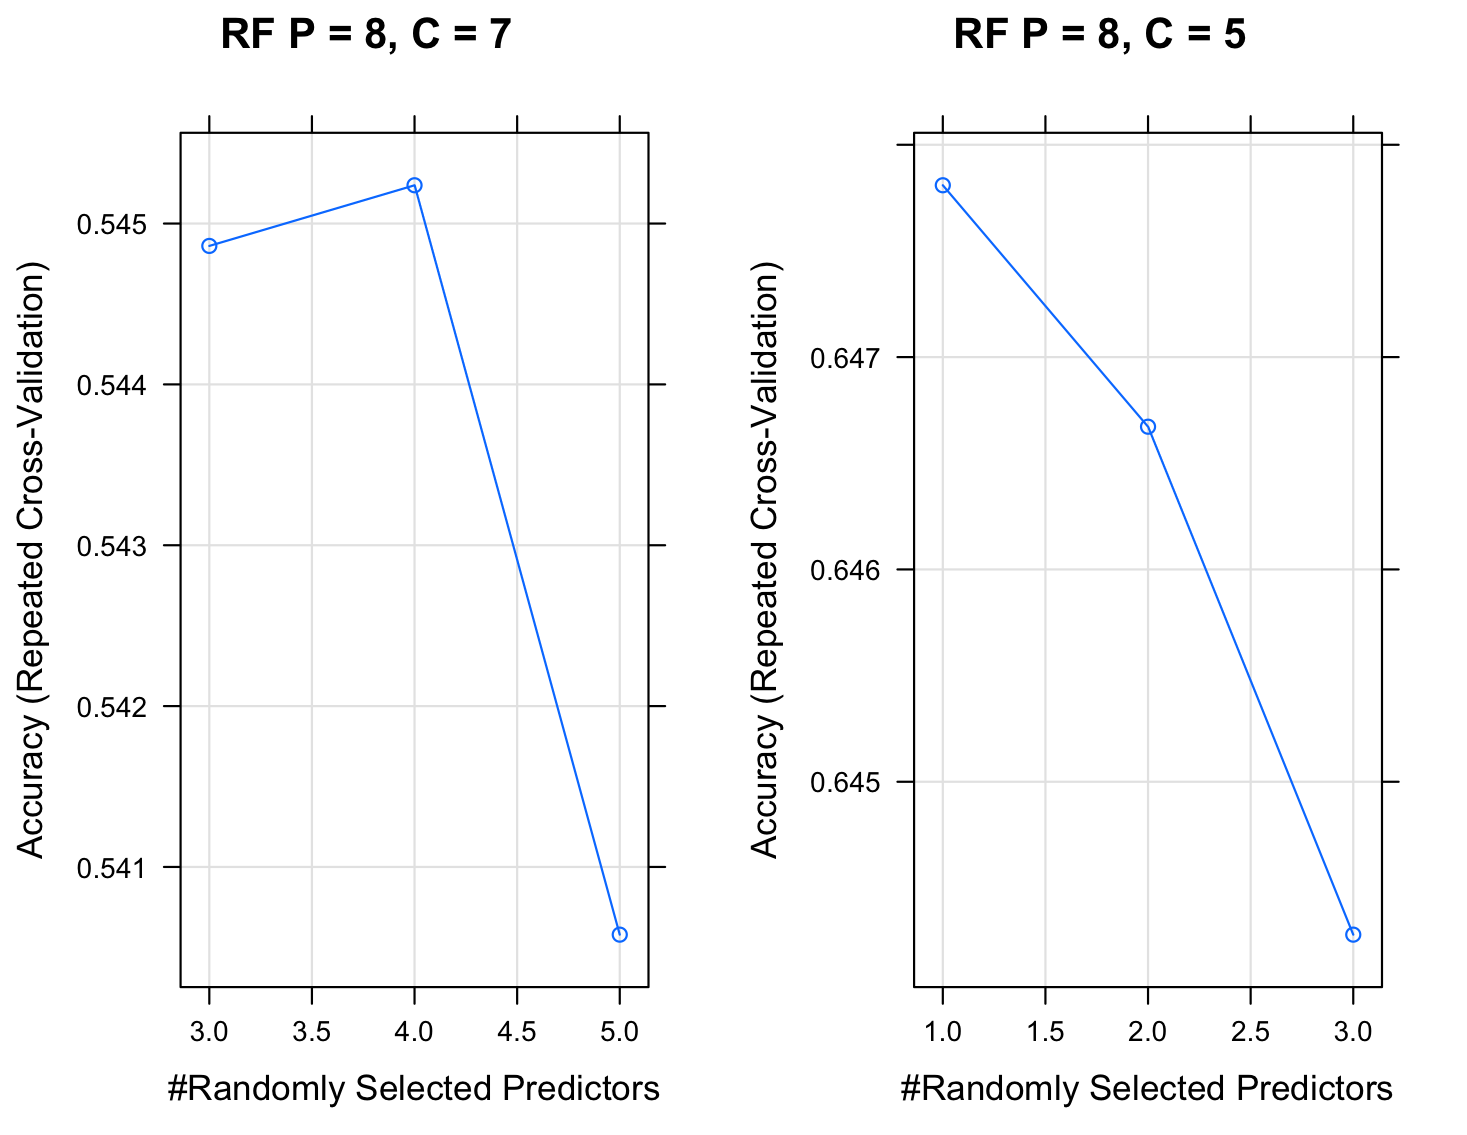
\includegraphics[width=0.9\linewidth]{figure/rf8_mtry} 

}

\caption{Accuracy of the 8 predictor trained random forest model for different mtry numbers over 10-fold cross-validation on 7 class and 5 class training data. (P = Predictors, C = Classes)}\label{fig:rf8}
\end{figure}
\hypertarget{predictor-random-forest-on-point-pixels}{%
\subsubsection{8 predictor Random Forest on Point Pixels}\label{predictor-random-forest-on-point-pixels}}

A RF model was trained using the 8 predictors from the previous model on the point pixels data. According to Figure \ref{fig:rf8c}, for modelling all 5 classes (Bigleaf Maple, Douglas-Fir, Giant Sequoia, Norway Maple, Western Redcedar), the optimal mtry value was 5 with an accuracy of 0.22. The variables with the higher predictive power were \(\frac{\mbox{red}}{\mbox{green}}\) and red band values predictors. The model using grouped data with 4 tree classes (Broadleaf, Douglas-Fir, Giant Sequoia, Western Redcedar), had an optimal mtry value of 1 with an accuracy of 0.33. The most important variable was \(\frac{\mbox{red}}{\mbox{green}}\).
\begin{figure}

{\centering 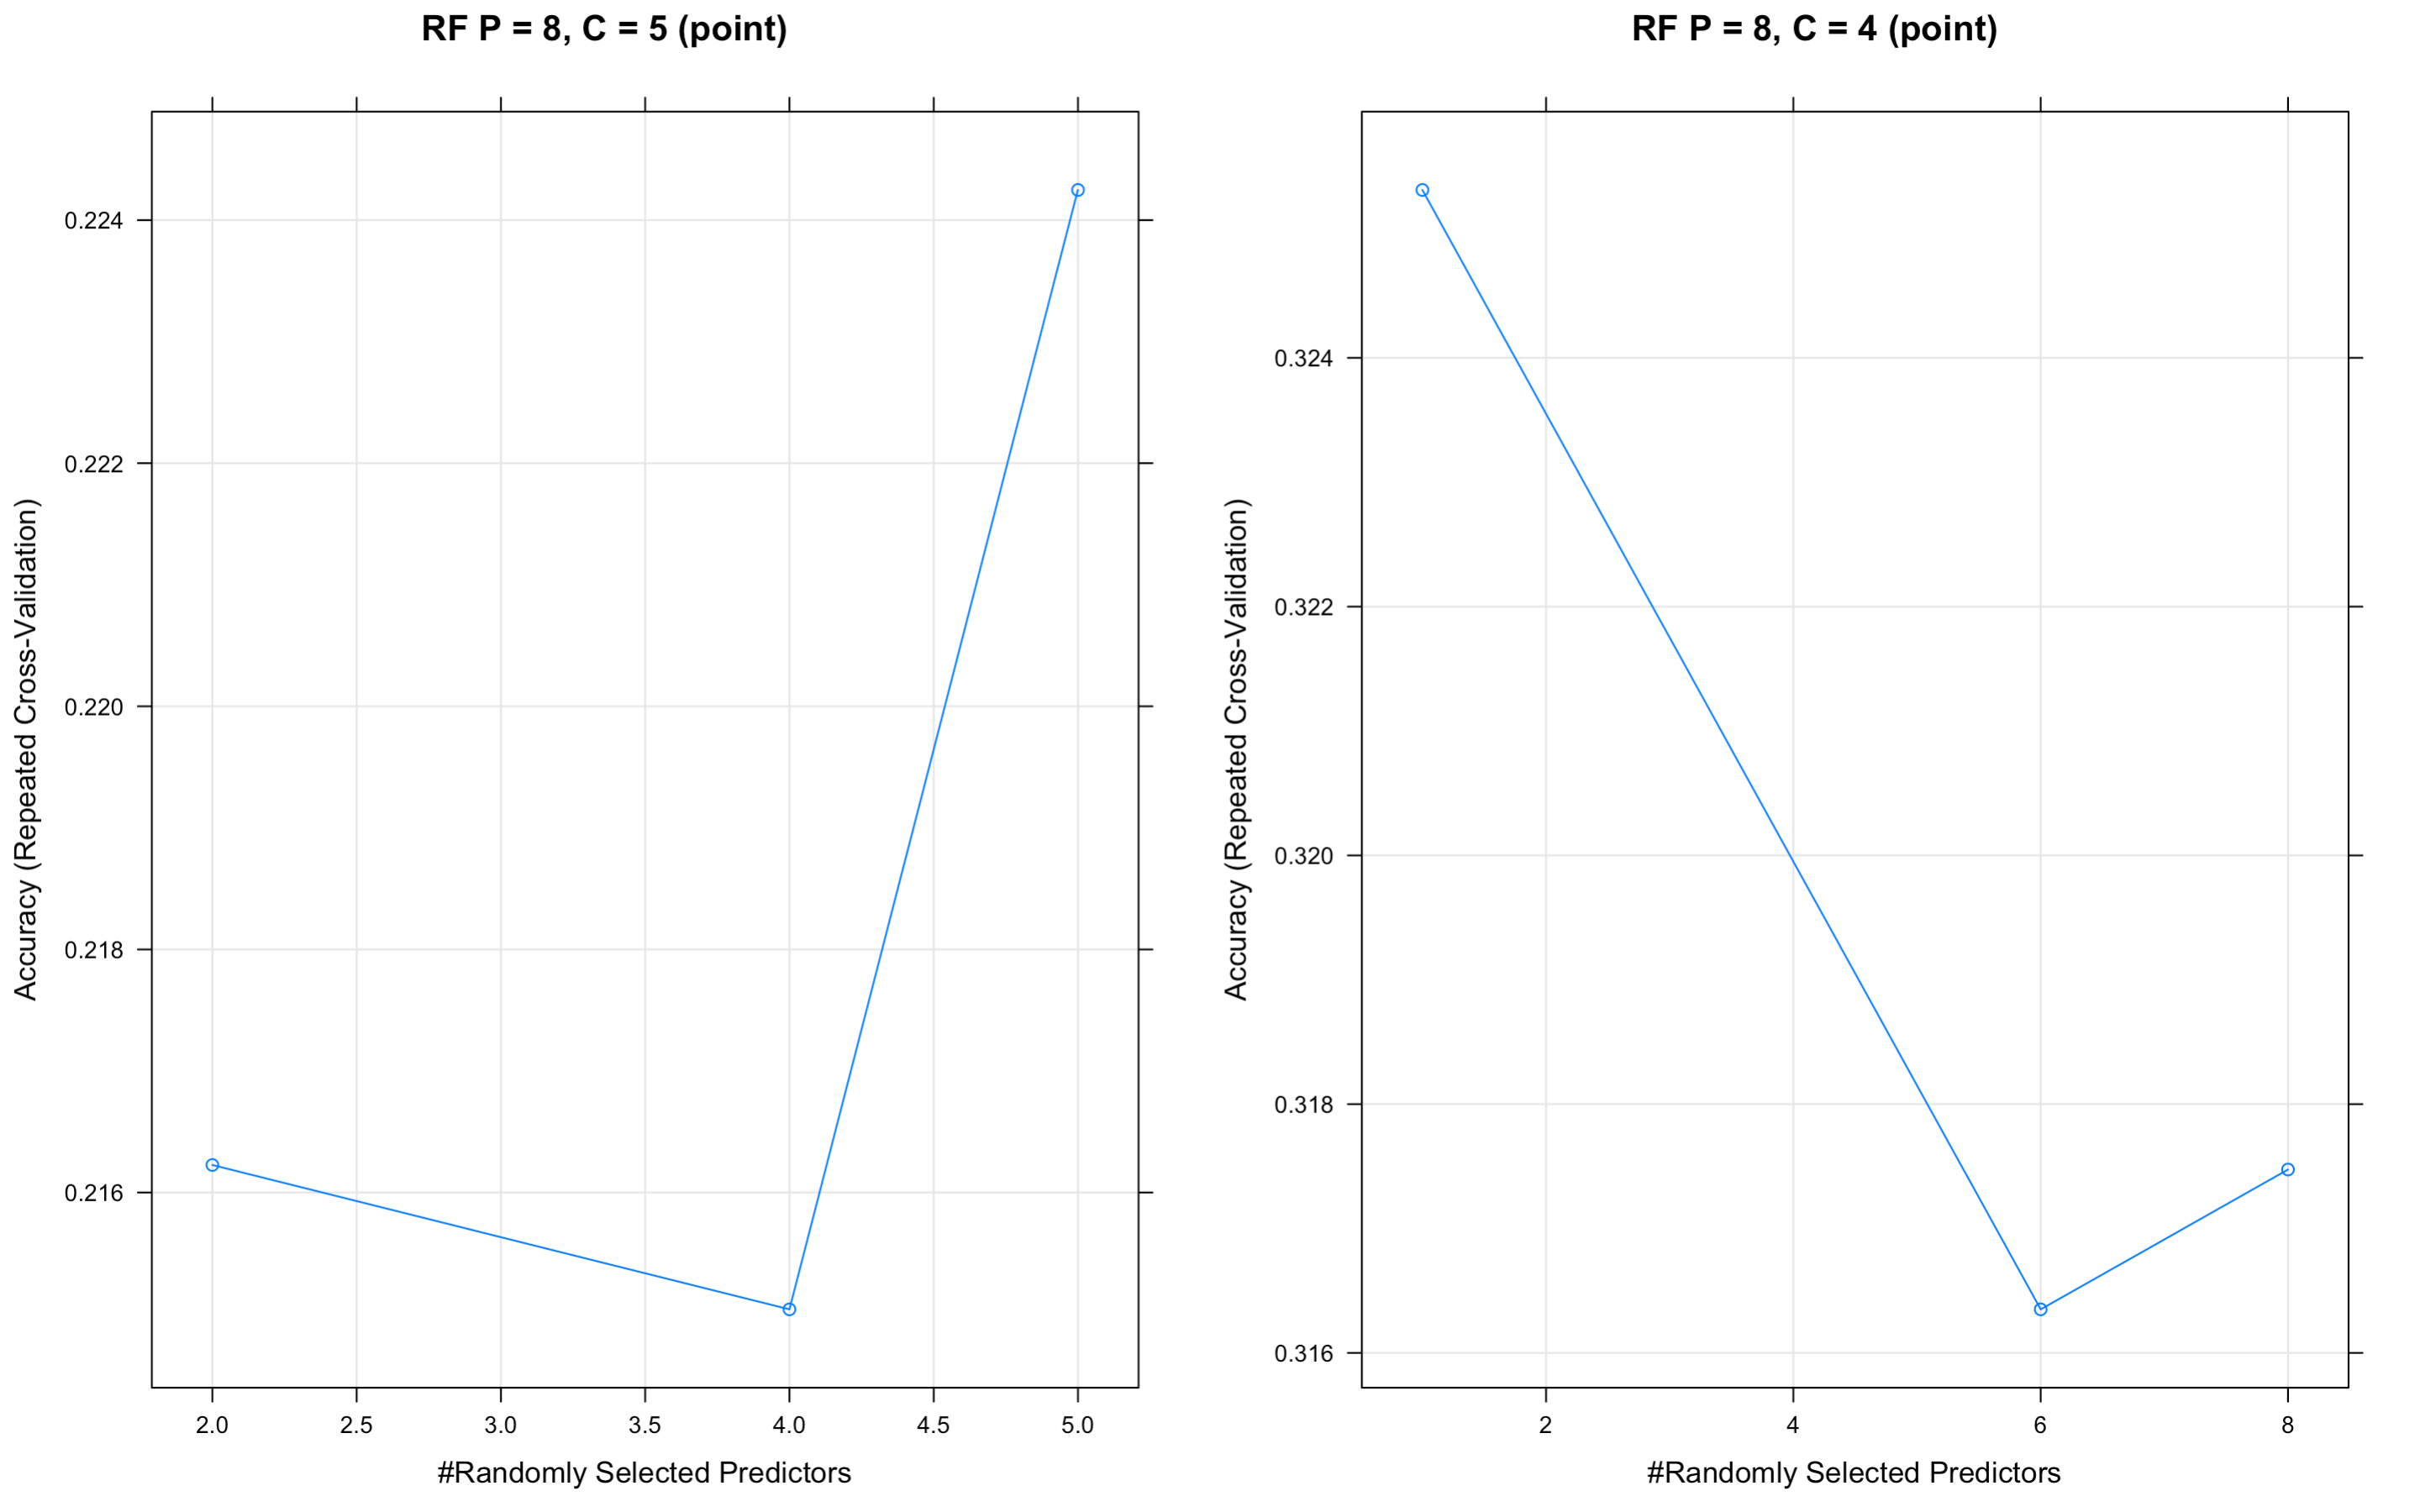
\includegraphics[width=0.9\linewidth]{figure/rf8c_mtry} 

}

\caption{Accuracy of the 8 predictor RF Model on point pixels data for different mtry numbers over 10-fold cross-validation on 5 class and 4 class training data. (P = Predictors, C = Classes)}\label{fig:rf8c}
\end{figure}
\hypertarget{best-random-forest}{%
\subsubsection{Best Random Forest}\label{best-random-forest}}

Figure \ref{fig:rfresults} compares the results of the models based on overall model accuracy in predicting the test data.
\begin{figure}

{\centering 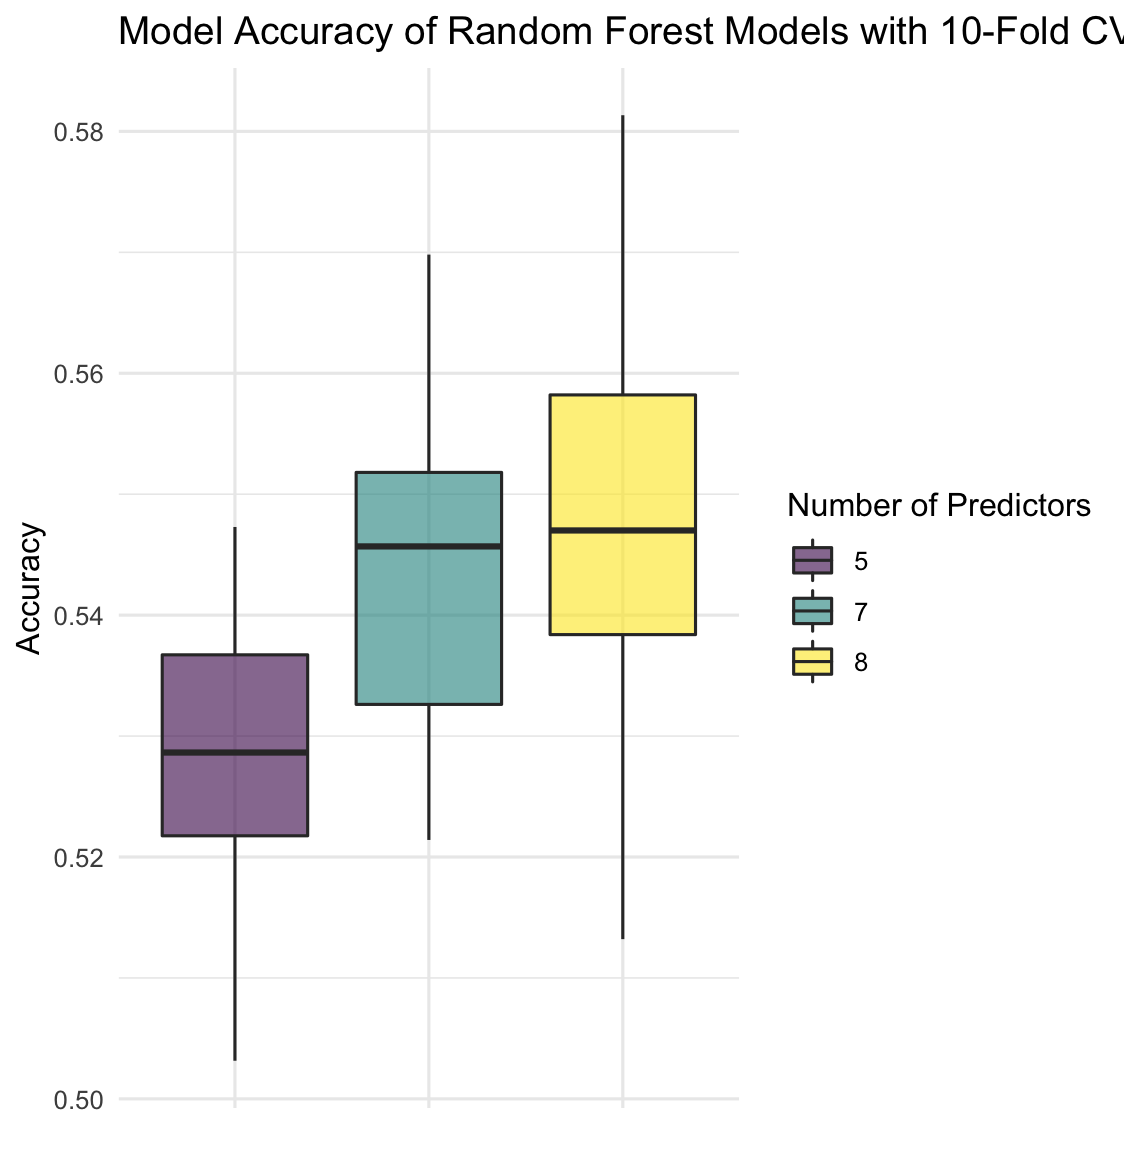
\includegraphics[width=0.9\linewidth]{figure/rfresults} 

}

\caption{Comparison of results from random forest models with different predictors included}\label{fig:rfresults}
\end{figure}
For modelling the 7 individual tree classes, the model with the 7 predictors included has a slightly higher maximum overall accuracy than the 8 predictor model. A confusion matrix located in Appendix \ref{tables} was constructed for each model averaging the entry counts over all ten cross validation resamples to investigate model performance just predicting Western Redcedar tree pixels. Both the 7 and the 8 predictor models performed similarly classifying Western Redceder pixels, the 7 predictor model had a prediction accuracy of 32\%, the 8 predictor model had a prediction accuracy of 33\%. Out of both models, Western Redcedars tend to be inaccurately classified under douglas-firs, english oak, and norway maple trees. The 8 predictor model trained on the point pixels data had a prediction accuracy of 29\% for 5 class predictions. This model also misclassified Western Redcedars as norway maples, giant sequoias, and bigleaf maples.

Modelling only 5 tree classes by grouping some categories produced higher overall accuracies than the full classes models. The 7 predictor and 8 predictor model produced the highest overall average accuracies of 0.57 through cross-validation. The 7 predictor model and the 8 predictor model accurately predicted Western Redcedars 36\% and 35\% of the time respectively. Most inaccurately predicted redcedars were classified under the broadleaf category. Models on both training sets predicted grass pixels with the highest accuracy. The 4 class model with the point pixel data had an overall accuracy of 0.33 with 0.25 Western Redcedar prediction accuracy.

Table \ref{tab:resultsRF} compares the hyperparameters accross all random forest models.
\begin{table}

\caption{\label{tab:resultsRF}Accuracy of random forest models with different number of predictors and mtry determined by ten-fold cross validation.}
\centering
\begin{tabular}[t]{l|r|r|r}
\hline
Random Forest Model & Accuracy & Kappa & mtry\\
\hline
P = 7, C = 7 & 0.4386 & 0.3450 & 1\\
\hline
P = 8, C = 7 & 0.4460 & 0.3537 & 4\\
\hline
P = 8, C = 5 (point) & 0.2242 & 0.0300 & 5\\
\hline
P = 7, C = 5 & 0.5740 & 0.3819 & 1\\
\hline
P = 8, C = 5 & 0.5666 & 0.3772 & 8\\
\hline
P = 8, C = 4 (point) & 0.3253 & 0.0024 & 1\\
\hline
\end{tabular}
\end{table}
\hypertarget{support-vector-machine-tuning}{%
\subsection{Support Vector Machine Tuning}\label{support-vector-machine-tuning}}

The \texttt{train} function has the \texttt{method\ =\ svmLinear/svmRadial/svmPoly} option to train a SVM model on the dataset to classify pixels into species of trees. For multiple class SVM training on \(k\) classes, this function classifies ``one-against-one'' by training \(k(k - 1)/2\) binary classifiers. This option also has parameters for cost, loss function, class weights, and normalized variables. For this project, three support vector machines were trained: linear, radial basis, and polynomial basis, and the preprocess setting for all three models were specified to center and scale (in R: \texttt{preProcess\ =\ c("center",\ "scale")}), which standardizes the variables. This is commonly performed with SVM models because the scale of the variables influences the optimal hyperplane decision. Since the light intensities extracted from the band data are only positive values, it is reasonable to consider normalizing the variables by setting the maximum value in the variable to 1 and the minimum value to 0, however, in comparing the SVM models under this preprocess setting (in R: \texttt{preProcess\ =\ "range"}) to the standardized setting, the accuracy of the models is not as high as the accuracy of the standardized variable models. The \texttt{caret} package selects the best cost tuning parameters based on accuracy through cross-validation.

\hypertarget{linear-support-vector-machine}{%
\subsubsection{Linear Support Vector Machine}\label{linear-support-vector-machine}}

The linear kernel SVM model had the highest training accuracy at 0.41 when cost parameter held constant at a value of 1. The final model contained 3017 support vectors. The linear kernel SVM model on the 5 classes data held the cost parameter constant at 1 predicted the grouped tree classes with an accuracy of 0.55 contained 2739 support vectors. The SVM model with point pixel data had an accuracy of 0.23 with C = 1 and 866 support vectors on 5 class data. On 4 class data, the linear SVM model with point pixel data had a prediction accuracy of 0.40 with C = 1 and 837 support vectors.

\hypertarget{radial-support-vector-machine}{%
\subsubsection{Radial Support Vector Machine}\label{radial-support-vector-machine}}

Figure \ref{fig:svm2} displays the results of different cost parameters on training accuracy for the radial basis kernel function on pixel data. The radial kernel SVM model on the 7 classes data set performed best when cost was 0.5 and \(\sigma = 0.27\) for a training accuracy of 0.45. The final model had 2972 support vectors. The final values for the radial model on the 5 classes data set were \(\sigma = 0.23\) and cost = 1 with an accuracy of 0.59 and 2630 support vectors. On the point pixels data, these values were C = 1, \(\sigma = 0.32\), overall accuracy of 0.21, and 868 support vectors for the 5 class model. For the 4 class model on the point pixels data, the values were C = 0.1, accuracy of 0.40, and 849 vectors. See figure \ref{fig:svm2c}.
\begin{figure}

{\centering 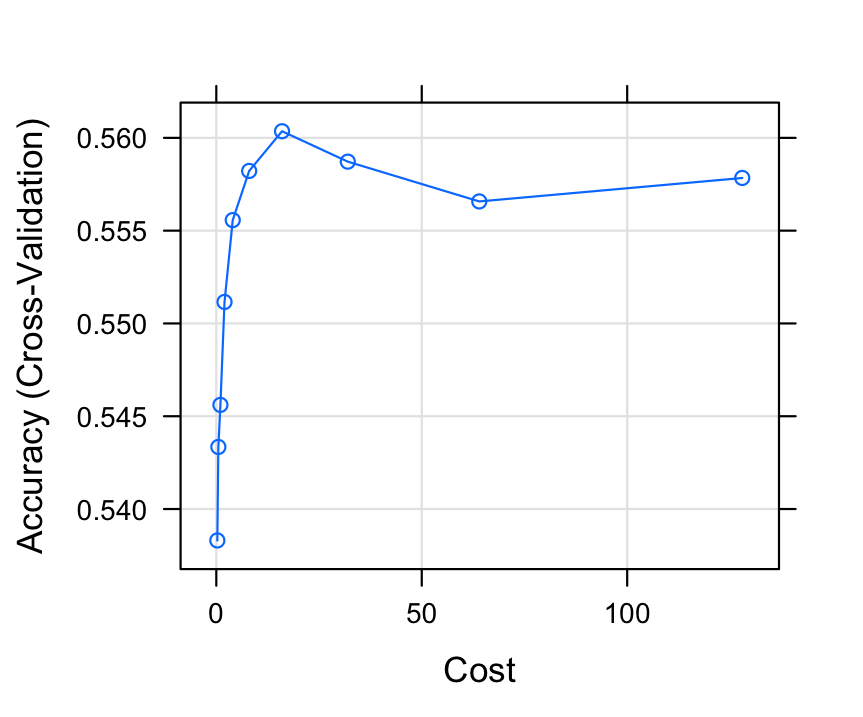
\includegraphics[width=0.9\linewidth]{figure/svm2} 

}

\caption{Comparison of accuracy results from different cost parameters for radial basis kernel function on pixel data.}\label{fig:svm2}
\end{figure}
\begin{figure}

{\centering 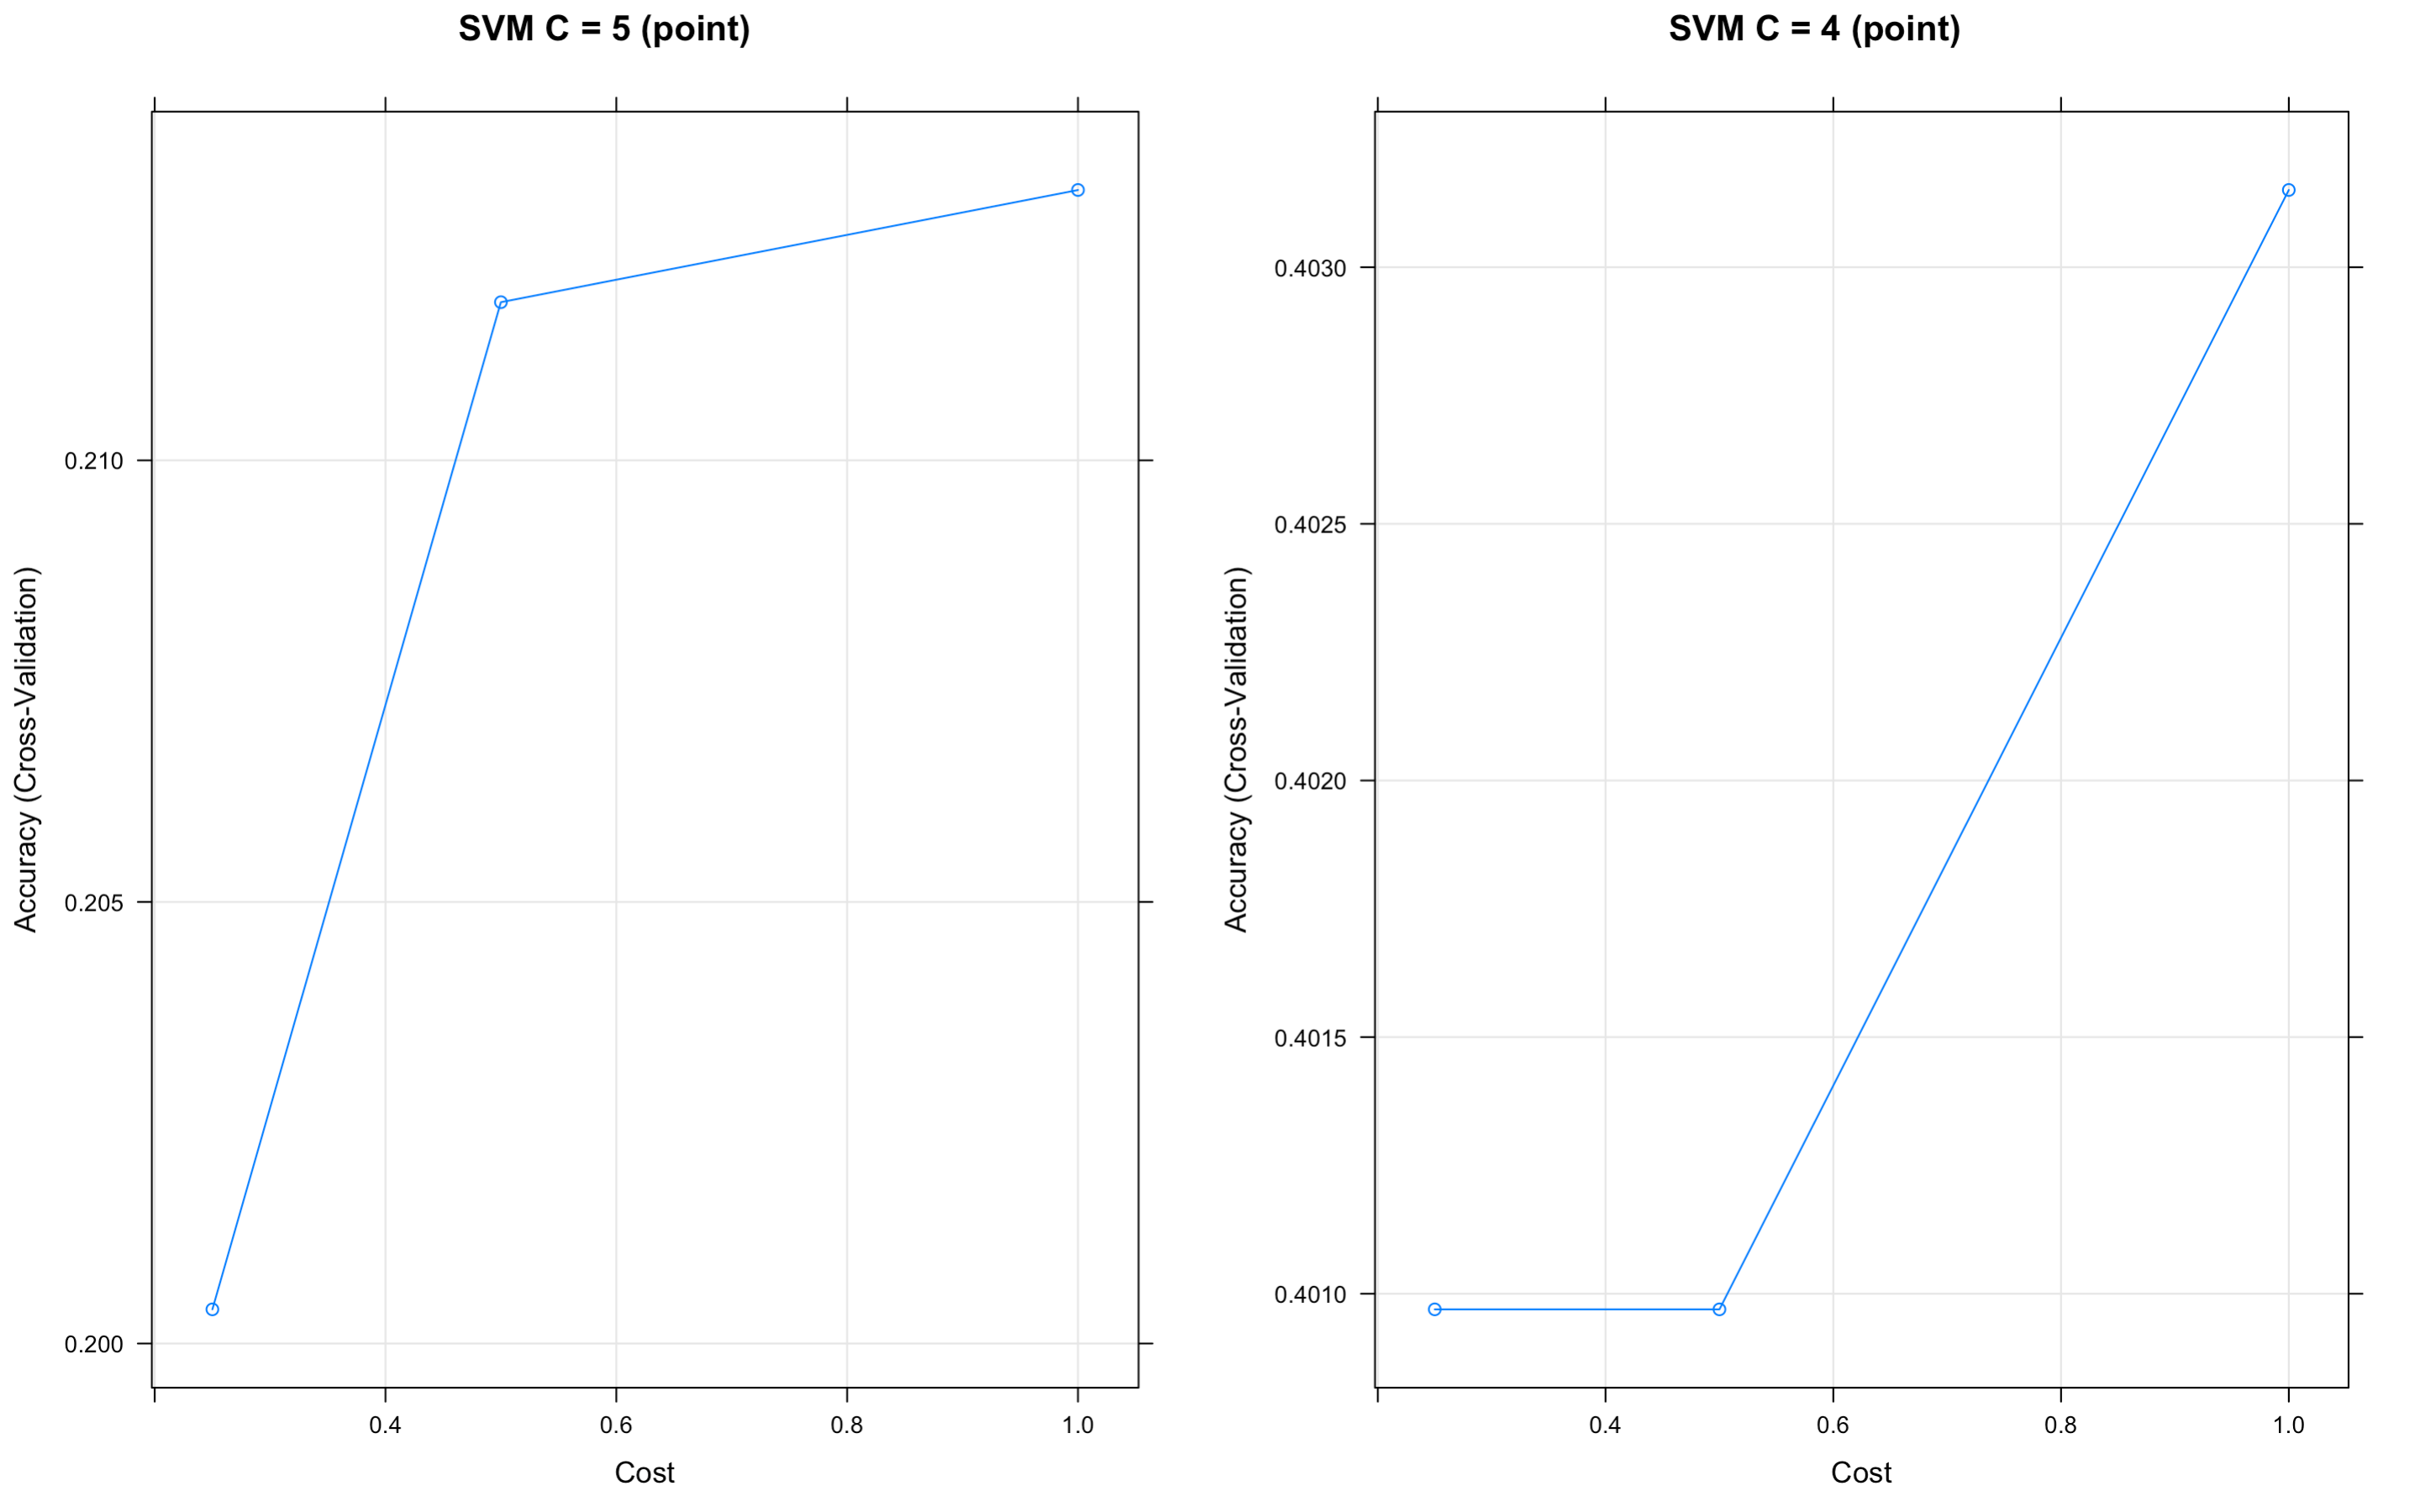
\includegraphics[width=0.9\linewidth]{figure/svm2c} 

}

\caption{Comparison of accuracy results from different cost parameters for radial basis kernel function on point pixel data.}\label{fig:svm2c}
\end{figure}
\hypertarget{polynomial-support-vector-machine}{%
\subsubsection{Polynomial Support Vector Machine}\label{polynomial-support-vector-machine}}

Figure \ref{fig:svm3} displays the results of different cost parameters on training accuracy for the polynomial basis function kernel. The final values used for the model predicting 7 classes were degree = 3, scale = 0.1, and cost = 1, which corresponded to a training accuracy of 0.44. The final model had a total of 2959 support vectors. The final model predicting only 5 classes produced an accuracy of 0.57 under degree = 3, scale = 0.1, and cost = 1. This final model had 2643 support vectors. Figure \ref{fig:svm3c} shows that the results for the point pixels data with 5 class predictions had an accuracy of 0.23 for degree = 1, scale = 0.1, cost = 1, and 869 support vectors. For 4 class predictions, the overall accuracy was 0.41 with degree = 3, scale = 0.1, cost = 0.1, and 852 support vectors.
\begin{figure}

{\centering 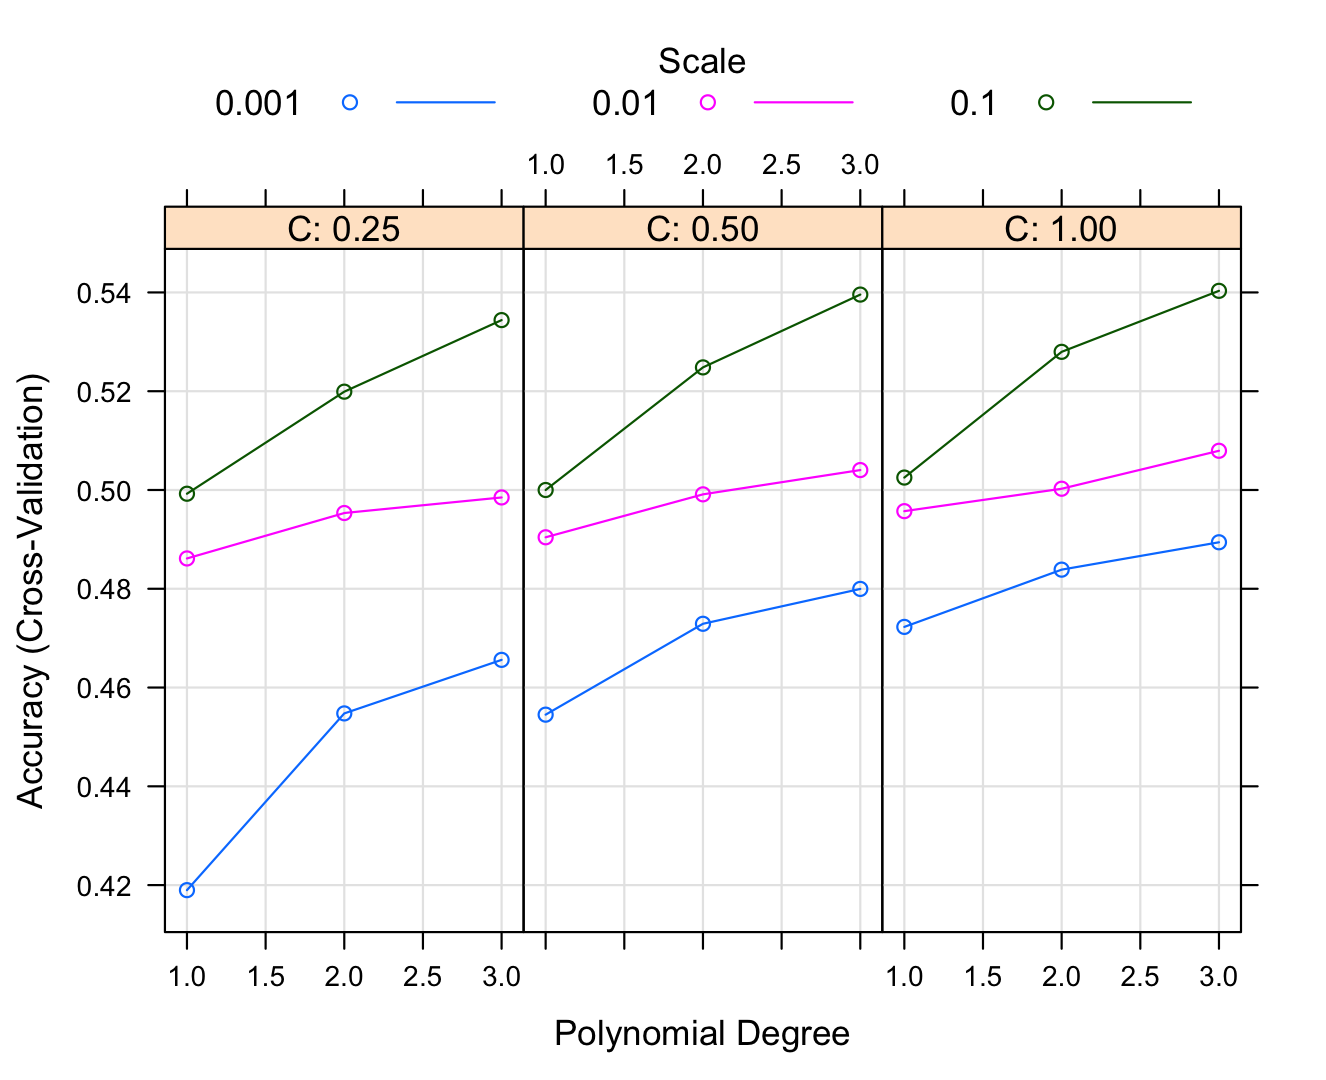
\includegraphics[width=0.9\linewidth]{figure/svm3} 

}

\caption{Comparison of accuracy results from different cost parameters with scale ranging from 0.001 to 0.1, C from 0.25 to 1, and degree from 1 to 3 for polynomial SVM on pixel data.}\label{fig:svm3}
\end{figure}
\begin{figure}

{\centering 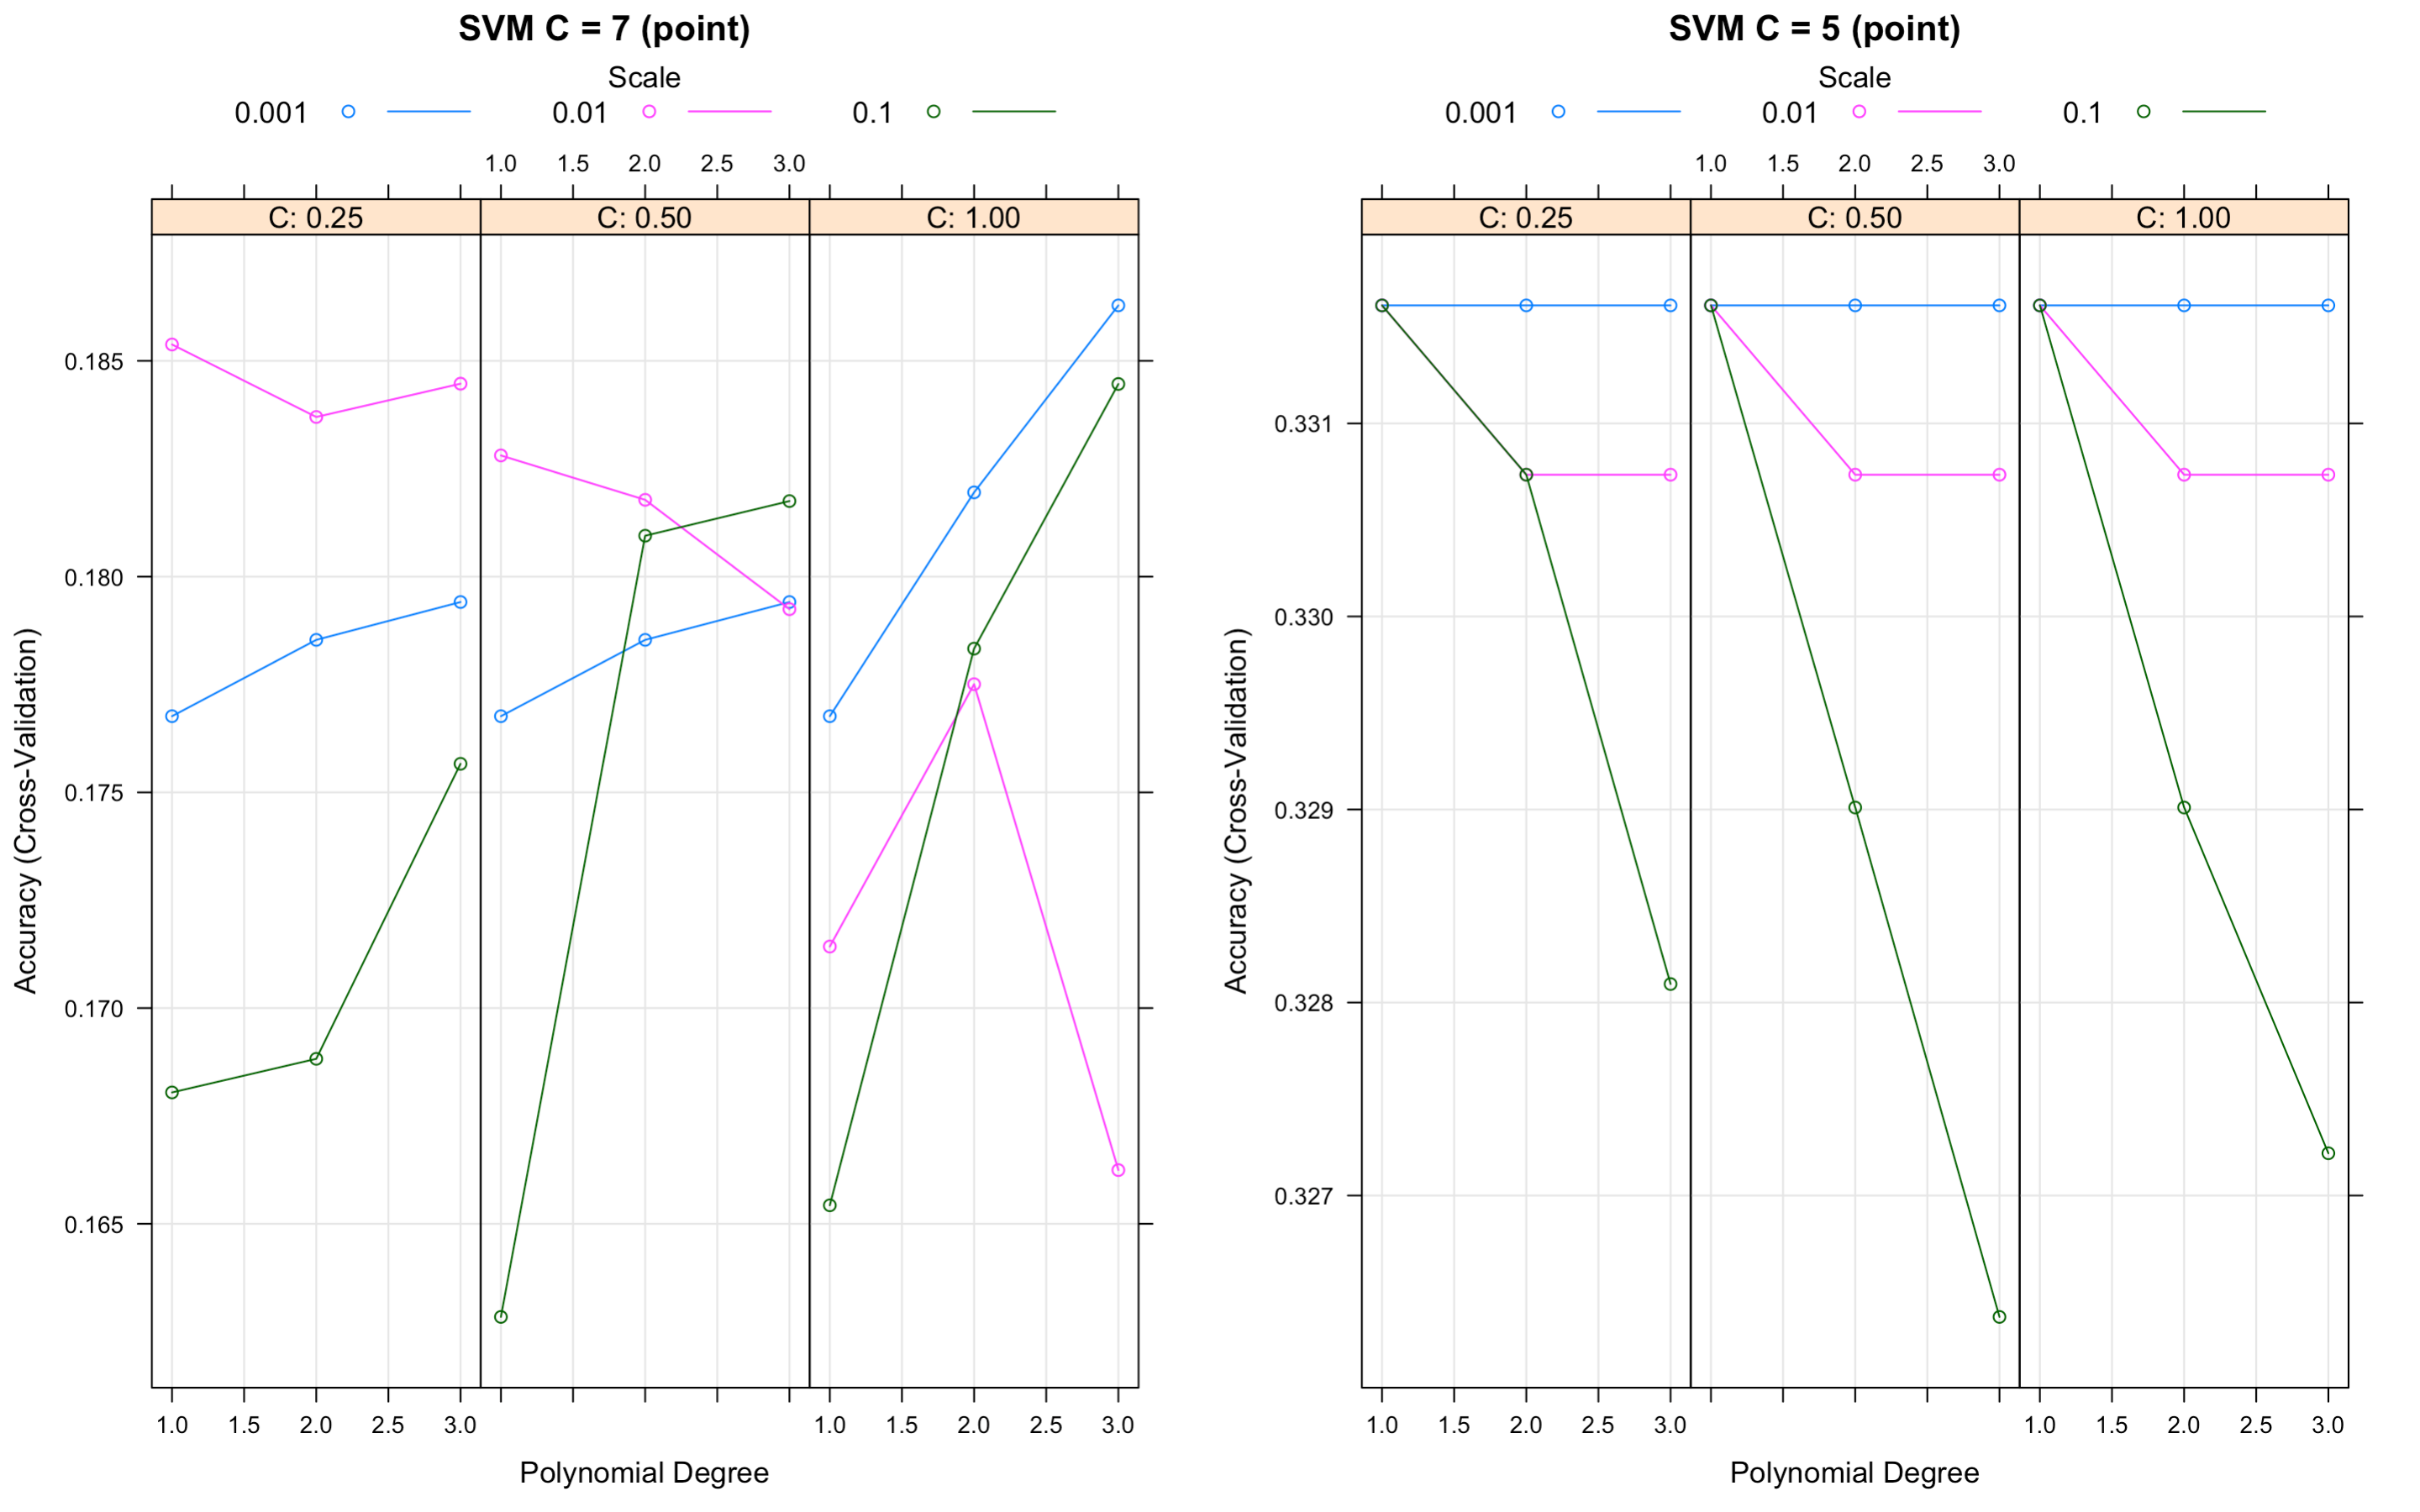
\includegraphics[width=0.9\linewidth]{figure/svm3c} 

}

\caption{Comparison of accuracy results from different cost parameters with scale ranging from 0.001 to 0.1, C from 0.25 to 1, and degree from 1 to 3 for polynomial SVM on point pixel data.}\label{fig:svm3c}
\end{figure}
\hypertarget{best-support-vector-machine}{%
\subsubsection{Best Support Vector Machine}\label{best-support-vector-machine}}

Figure \ref{fig:svmresults} displays the results of the linear, radial basis, and polynomial basis support vector machine models. Based on the overall prediction accuracy, the radial basis is an appropriate kernel choice for the pixels data with the 5 class prediction.
\begin{figure}

{\centering 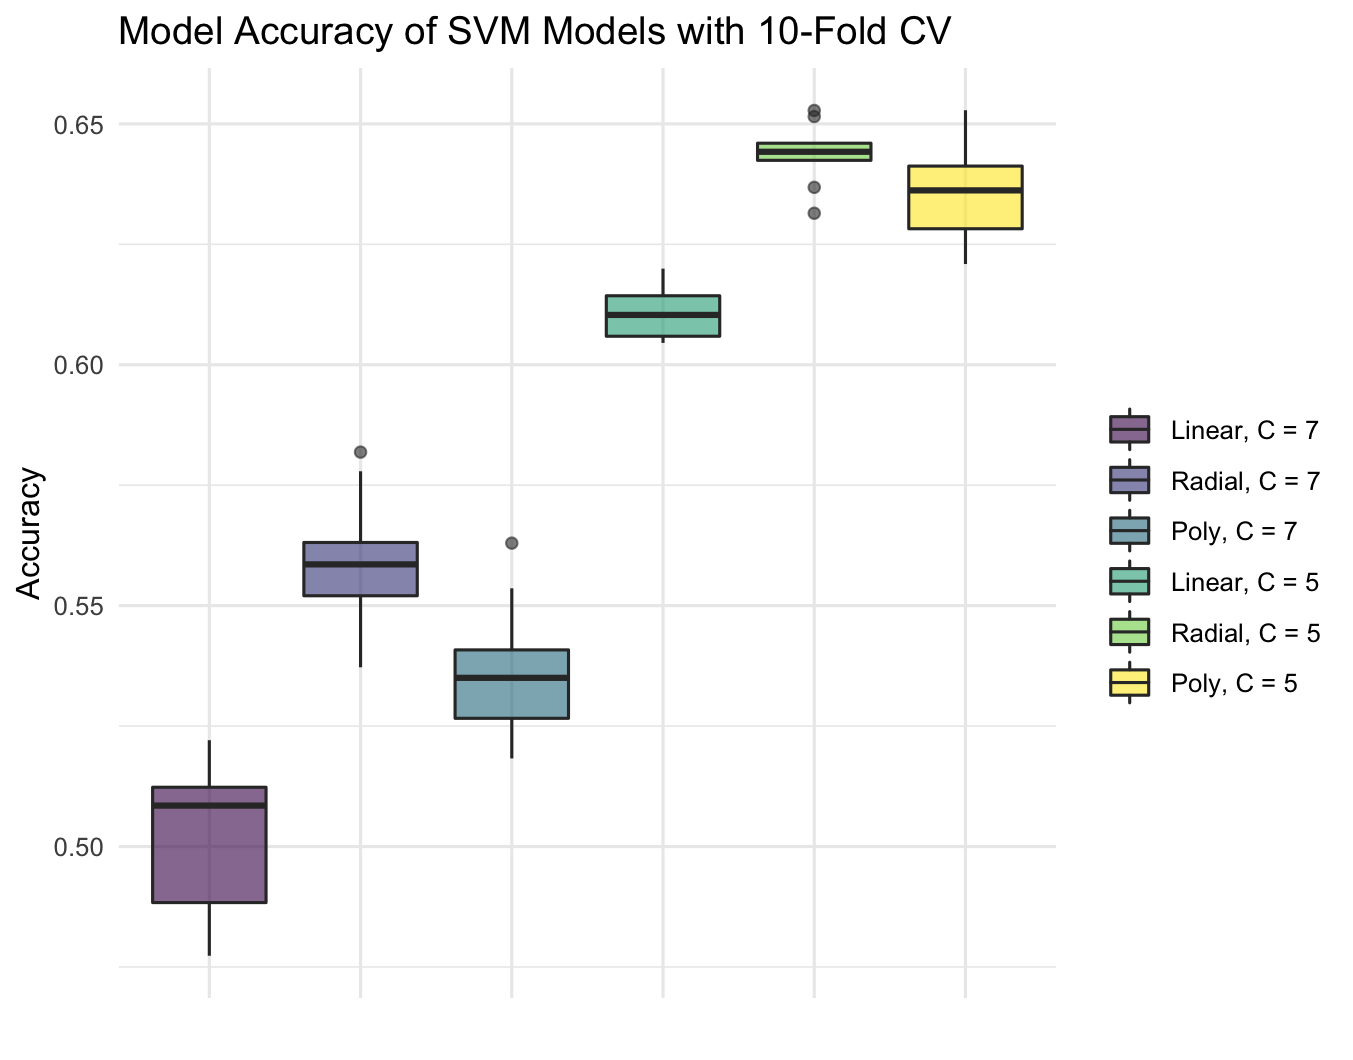
\includegraphics[width=0.9\linewidth]{figure/svmresults} 

}

\caption{Comparison of results from support vector machine models with different kernel types: linear, radial, and polynomial.}\label{fig:svmresults}
\end{figure}
As with the random forest model comparisons, a confusion matrix (Appendix \ref{tables}) was constructed using the average counts over all ten cross-validation resamples to obtain the model results predicting Western Redcedars. The support vector machine model that performed best overall was the radial basis kernel model, and it had a prediction accuracy of 35\% for the Western Redcedar class. The polynomial basis kernel had a 34\% prediction accuracy and the linear kernel also had an accuracy of 33\% for Western Redcedars. For Western Redcedar prediction on the grouped classes, the radial model had 44\% accuracy. The highest Western Redcedar prediction accuracy for SVM models with point pixel training data was for the polynomial basis model at 24\%.

Table \ref{tab:resultsSVM} compares the hyperparameters accross all support vector machine models.
\begin{table}

\caption{\label{tab:resultsSVM}Accuracy of support vector machine models with different kernels. Best parameter is determined by ten-fold cross validation.}
\centering
\begin{tabular}[t]{l|r|r}
\hline
SVM Model Kernel & Accuracy & Kappa\\
\hline
Linear, C = 7 & 0.4100 & 0.3117\\
\hline
Radial, C = 7 & 0.4534 & 0.3623\\
\hline
Poly, C = 7 & 0.4449 & 0.3523\\
\hline
Linear, C = 5 (point) & 0.2314 & 0.0402\\
\hline
Radial, C = 5 (point) & 0.2131 & 0.0169\\
\hline
Poly, C = 5 (point) & 0.2382 & 0.0484\\
\hline
Linear, C = 5 & 0.5486 & 0.2778\\
\hline
Radial, C = 5 & 0.5860 & 0.3675\\
\hline
Poly, C = 5 & 0.5729 & 0.3310\\
\hline
Linear, C = 4 (point) & 0.4009 & 0.0000\\
\hline
Radial, C = 4 (point) & 0.4032 & 0.0120\\
\hline
Poly, C = 4 (point) & 0.4067 & 0.0140\\
\hline
\end{tabular}
\end{table}
\hypertarget{testing-models}{%
\section{Testing Models}\label{testing-models}}

A subset of the data was withheld from training the models as test data to provide some measure of how the models perform in predicting results on new data. Based on overall and redcedar accuracy, the appropriate models to consider with the testing data are the 5 class 7 predictor RF and the 5 class radial SVM. The results for the overall test accuracy and the prediction test accuracy for Western Redcedars are shown in Tables \ref{tab:resultsTestRF} and \ref{tab:resultsTestSVM}.
\begin{table}[!h]

\caption{\label{tab:resultsTestRF}Overall accuracy of 7 predictor RF (5 class) model on test data}
\centering
\resizebox{\linewidth}{!}{
\begin{tabular}[t]{l|>{\raggedleft\arraybackslash}p{0.6in}|>{\raggedleft\arraybackslash}p{0.6in}|>{\raggedleft\arraybackslash}p{0.6in}|>{\raggedleft\arraybackslash}p{0.6in}|>{\raggedleft\arraybackslash}p{0.6in}|>{\raggedleft\arraybackslash}p{0.6in}|>{\raggedleft\arraybackslash}p{0.6in}|>{\raggedleft\arraybackslash}p{0.6in}|>{\raggedleft\arraybackslash}p{0.6in}|>{\raggedleft\arraybackslash}p{0.6in}|>{\raggedleft\arraybackslash}p{0.6in}}
\hline
  & Sensitivity & Specificity & Pos Pred Value & Neg Pred Value & Precision & Recall & F1 & Prevalence & Detection Rate & Detection Prevalence & Balanced Accuracy\\
\hline
Class: Broadleaf & 0.78 & 0.68 & 0.57 & 0.85 & 0.57 & 0.78 & 0.66 & 0.35 & 0.27 & 0.48 & 0.73\\
\hline
Class: Douglas-Fir & 0.32 & 0.96 & 0.52 & 0.92 & 0.52 & 0.32 & 0.40 & 0.11 & 0.04 & 0.07 & 0.64\\
\hline
Class: Giant Sequoia & 0.23 & 0.96 & 0.45 & 0.90 & 0.45 & 0.23 & 0.31 & 0.12 & 0.03 & 0.06 & 0.60\\
\hline
Class: grass & 0.95 & 0.96 & 0.92 & 0.98 & 0.92 & 0.95 & 0.93 & 0.31 & 0.29 & 0.32 & 0.95\\
\hline
Class: Western Redcedar & 0.22 & 0.95 & 0.35 & 0.91 & 0.35 & 0.22 & 0.27 & 0.11 & 0.02 & 0.07 & 0.58\\
\hline
\end{tabular}}
\end{table}
\begin{table}[!h]

\caption{\label{tab:resultsTestSVM}Overall accuracy of Radial SVM (5 class) model on test data}
\centering
\resizebox{\linewidth}{!}{
\begin{tabular}[t]{l|>{\raggedleft\arraybackslash}p{0.6in}|>{\raggedleft\arraybackslash}p{0.6in}|>{\raggedleft\arraybackslash}p{0.6in}|>{\raggedleft\arraybackslash}p{0.6in}|>{\raggedleft\arraybackslash}p{0.6in}|>{\raggedleft\arraybackslash}p{0.6in}|>{\raggedleft\arraybackslash}p{0.6in}|>{\raggedleft\arraybackslash}p{0.6in}|>{\raggedleft\arraybackslash}p{0.6in}|>{\raggedleft\arraybackslash}p{0.6in}|>{\raggedleft\arraybackslash}p{0.6in}}
\hline
  & Sensitivity & Specificity & Pos Pred Value & Neg Pred Value & Precision & Recall & F1 & Prevalence & Detection Rate & Detection Prevalence & Balanced Accuracy\\
\hline
Class: Broadleaf & 0.87 & 0.58 & 0.53 & 0.90 & 0.53 & 0.87 & 0.66 & 0.35 & 0.31 & 0.58 & 0.73\\
\hline
Class: Douglas-Fir & 0.22 & 0.99 & 0.73 & 0.91 & 0.73 & 0.22 & 0.33 & 0.11 & 0.02 & 0.03 & 0.60\\
\hline
Class: Giant Sequoia & 0.15 & 0.98 & 0.50 & 0.90 & 0.50 & 0.15 & 0.23 & 0.12 & 0.02 & 0.04 & 0.57\\
\hline
Class: grass & 0.96 & 0.96 & 0.91 & 0.98 & 0.91 & 0.96 & 0.94 & 0.31 & 0.30 & 0.33 & 0.96\\
\hline
Class: Western Redcedar & 0.11 & 0.98 & 0.47 & 0.90 & 0.47 & 0.11 & 0.18 & 0.11 & 0.01 & 0.03 & 0.55\\
\hline
\end{tabular}}
\end{table}
According to the test data, the best performing models for further analysis are the radial SVM model for 5 class prediction and the 7 predictor RF model for 5 class prediction.

The polygon prediction accuracy on the test dataset was also computed to see how pixels of the same tree were classified compared to individual pixel classification. A ``correct'' prediction was indicated if more than half the pixels in a polygon are correctly predicted. Table \ref{tab:polyTab} displays the overall results for polygons in the test dataset and Table \ref{tab:polyTabRed} displays the polygons predictions for Western Redcedars.
\begin{table}

\caption{\label{tab:polyTab}Overall accuracy of radial SVM model with 5 classes and 7 predictor RF model with 5 classes for polygons in test data. A correct prediction is considered to be a polygon with more than half of the pixels correctly classified.}
\centering
\begin{tabular}[t]{l|l|r}
\hline
Type & Result & Polygons\\
\hline
SVM C = 5 & Correct & 362\\
\hline
SVM C = 5 & Incorrect & 311\\
\hline
RF P = 7, C = 5 & Correct & 349\\
\hline
RF P = 7, C = 5 & Incorrect & 324\\
\hline
\end{tabular}
\end{table}
\begin{table}

\caption{\label{tab:polyTabRed}Western Redcedar accuracy of radial SVM model with 5 classes and 7 predictor RF model with 5 classes for polygons in test data. A correct prediction is considered to be a polygon with more than half of the pixels correctly classified.}
\centering
\begin{tabular}[t]{l|l|r}
\hline
Type & Result & Polygons\\
\hline
SVM C = 5 & Correct & 7\\
\hline
SVM C = 5 & Incorrect & 93\\
\hline
RF P = 7, C = 5 & Correct & 8\\
\hline
RF P = 7, C = 5 & Incorrect & 92\\
\hline
\end{tabular}
\end{table}
\hypertarget{results}{%
\chapter{Results}\label{results}}

\hypertarget{training-results}{%
\section{Training Results}\label{training-results}}

Predicting on the grouped data produced the highest overall accuracies. The best model on the grouped data was the RF training model with an mtry value of 3 predictors at each split and the following predictors: red, green, blue, infrared, NDVI, \(\frac{\mbox{red}}{\mbox{green}}\), \(\frac{\mbox{red}}{\mbox{blue}}\). This model had a training predictive accuracy of 0.57 overall and 0.36 for Western Redcedars specifically. On the test dataset, this model accurately predicted 65\% of the pixels, 22\% of Western Redcedars, while the accuracy for predicting more than half the pixels correctly in the same polygon was 52\%.

The model that performed best among SVM models was the radial SVM on 5 class data. This model had a training accuracy of 0.59 overall, 0.35 for just Western Redcedars, and testing accuracy of 0.66 overall and 0.11 for Western Redcedar pixels. For polygon predictions, the radial SVM C = 5 model had an accuracy of 54\%. Both models perform similarly, however, for Western Redcedar predictions, the RF model outperforms the SVM model. These models are used to proceed with the final model over Portland.

\hypertarget{modelling-tree-species-in-portland}{%
\section{Modelling Tree Species in Portland}\label{modelling-tree-species-in-portland}}

After masking the raster images of the entire region of Portland by NDVI values, the pre-trained models are used to predict the tree species of individual pixels in the masked raster images. The \texttt{predict.raster} function from RStudio's \texttt{raster} package takes a model and applies that model to each cell of the raster, leaving a raster with tree classification predictions. This function is used to predict tree species over all five raster strips, and the raster strips are merged to display predictions for the entire city. Figure \ref{fig:rfPortlandRF} displays the tree classification predictions given by the optimal random forest model over Portland and figure \ref{fig:rfPortlandSVM} displays the predictions from the support vector machine model.
\begin{figure}

{\centering 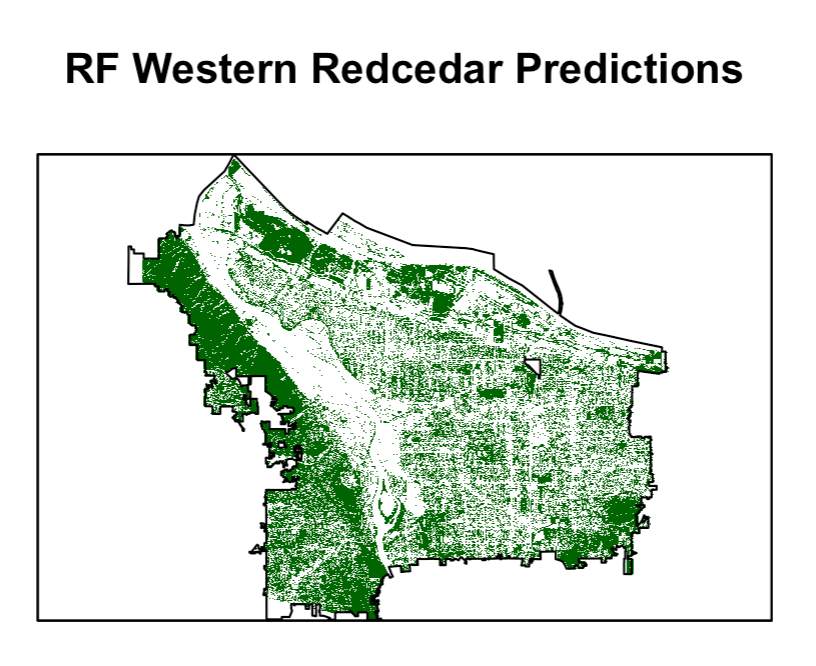
\includegraphics[width=1\linewidth]{figure/rfPortland} 

}

\caption{Model tree classification predictions of Western Redcedars over entire Portland region using the random forest model with 7 predictors on 5 classes.}\label{fig:rfPortlandRF}
\end{figure}
\begin{figure}

{\centering 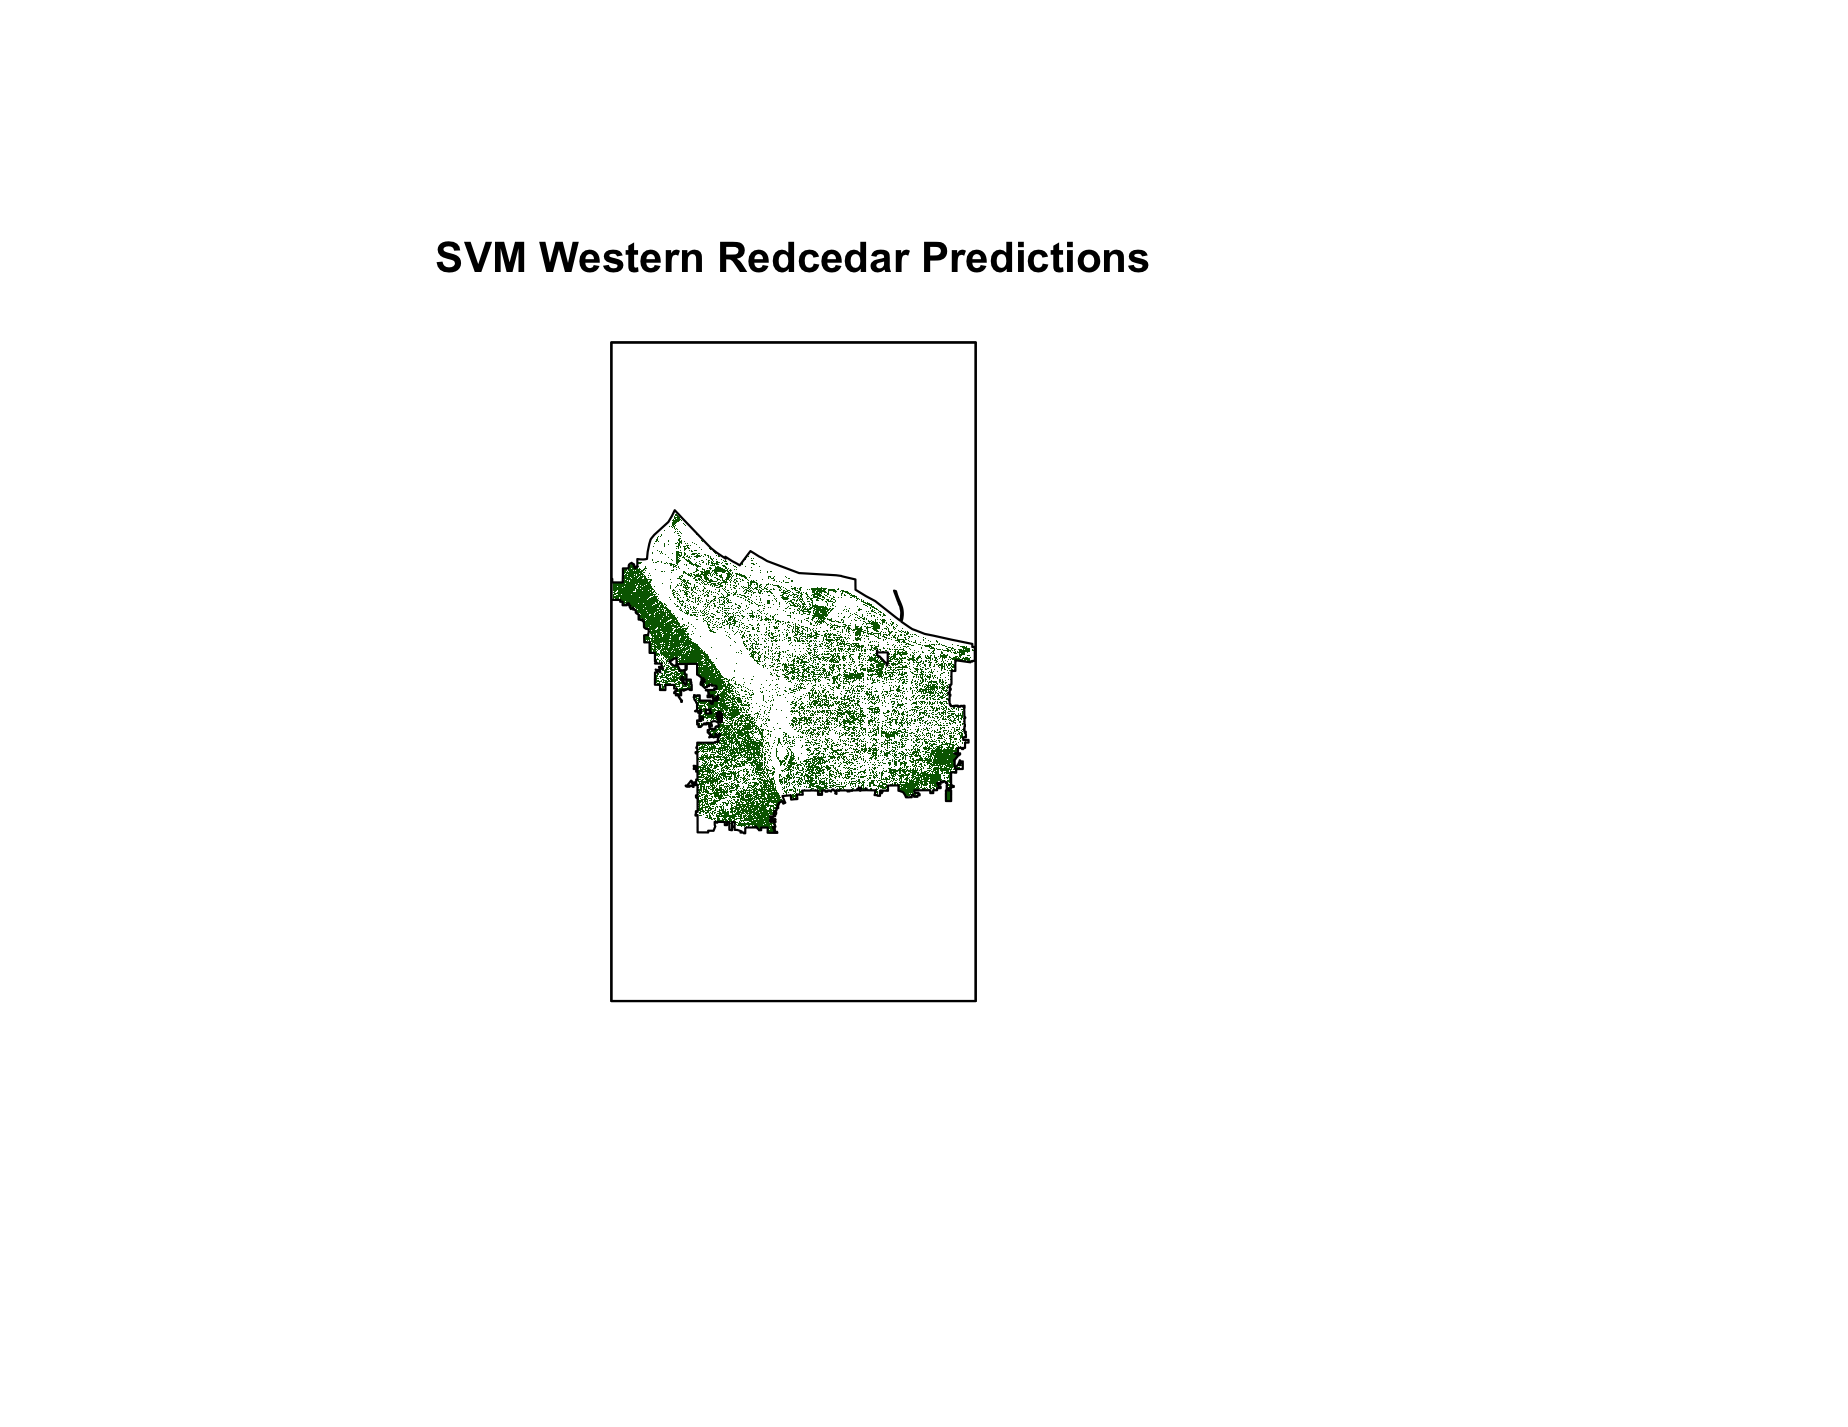
\includegraphics[width=1\linewidth]{figure/svmPortland} 

}

\caption{Model tree classification predictions of Western Redcedars over entire Portland region using radial SVM C = 5.}\label{fig:rfPortlandSVM}
\end{figure}
In comparing the RF P = 7, C = 5 model results to the radial SVM C = 5 results, 91\% of the Western Redcedar pixel predictions were the same predictions under both models.

To assess the performance of the model over the Portland region, the results are compared to the remaining Western Redcedars from \texttt{pdxTrees} both street and park data. The shapefiles for \texttt{pdxTrees} Western Redcedars ground data are mapped over the classified pixel predictions, and the number of correctly and incorrectly classified pixels is recorded to be 57\% accurate for RF P = 7, C = 5 and 63\% accurate for radial SVM C = 5. Figure \ref{fig:resultsToStreet} visualizes this comparison for RF P = 7, C = 5.
\begin{figure}

{\centering 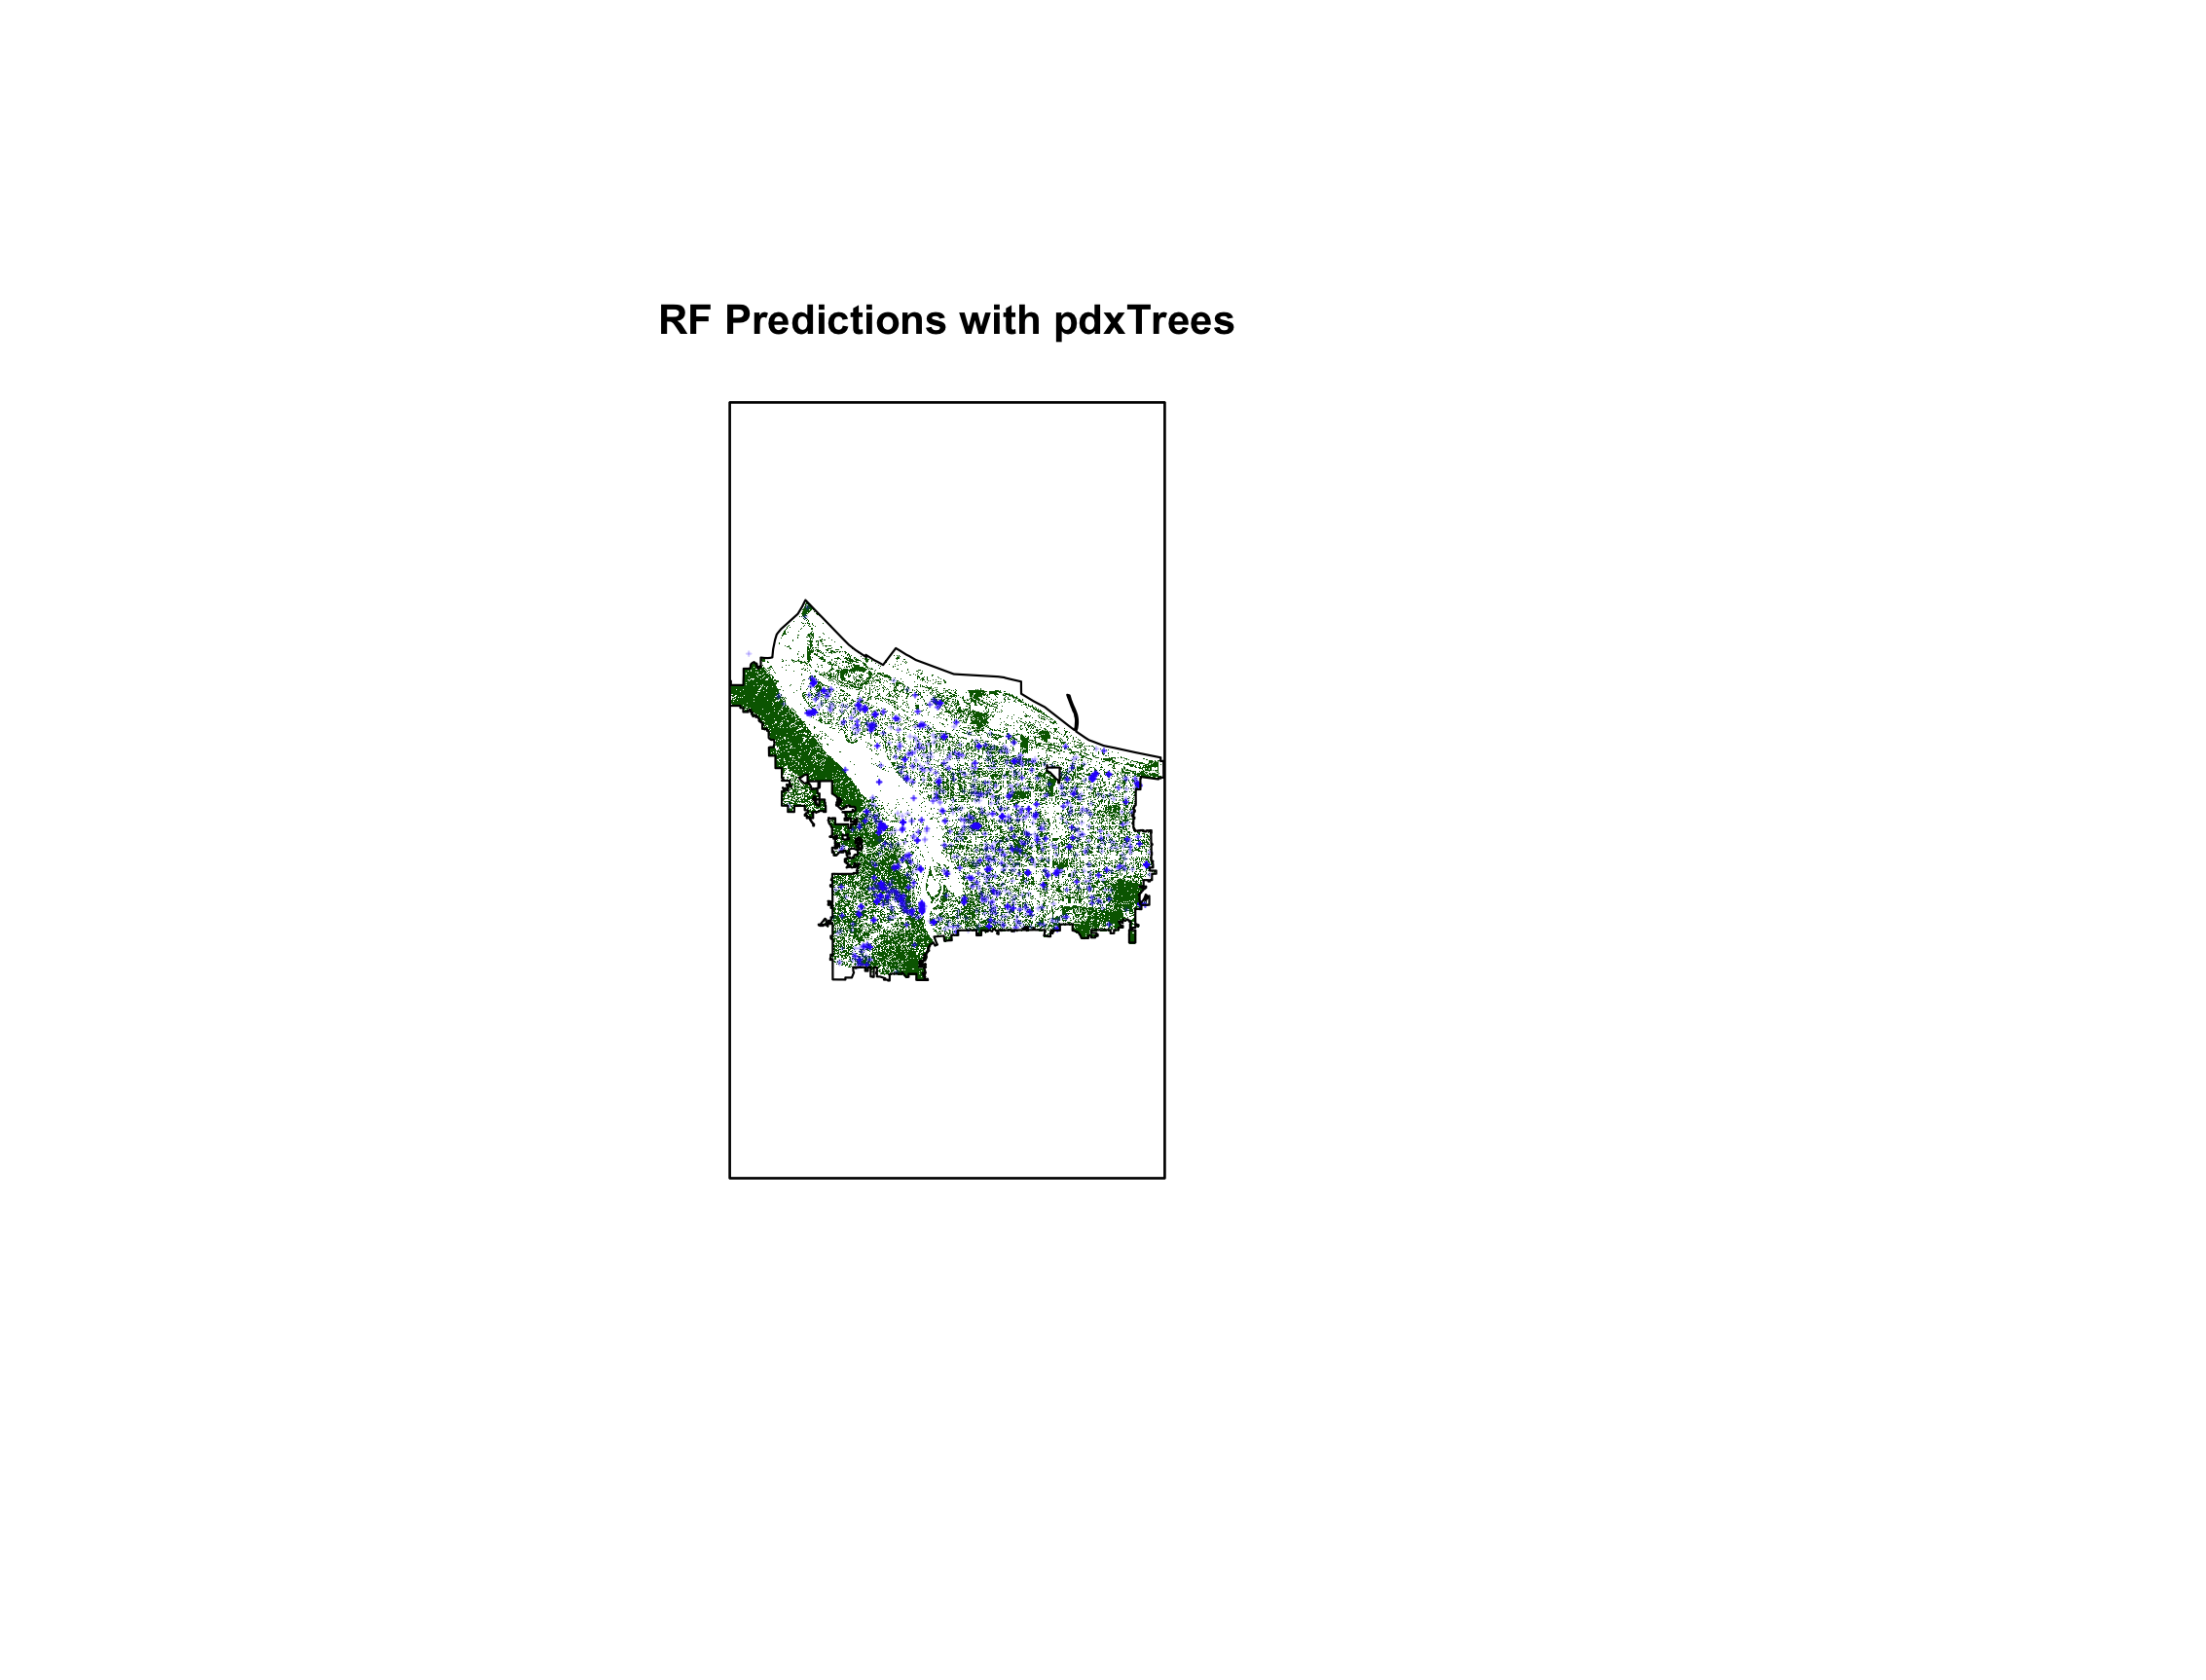
\includegraphics[width=1\linewidth]{figure/resultsToStreet} 

}

\caption{Comparison of Wester redcedar RF pixel predictions (in green) to Western Redcedar trees from pdxTrees (in blue).}\label{fig:resultsToStreet}
\end{figure}
As part of the research seeks to investigate whether tree prediction outside of Portland's Tree Inventory Project is possible, Figure \ref{fig:reedTreesTopdx} presents a side-by-side comparison of tree predictions for trees in proximity to Reed College. As part of the Tree Inventory Project, the trees are mapped on a satellite image at a higher resolution than used in this research, and the left image in Figure \ref{fig:reedTreesTopdx} displays which trees are included in the citywide study (``Tree Inventory Project,'' n.d.). The right image in Figure \ref{fig:reedTreesTopdx} displays model predictions for trees in the same region. Pixels in green accurately indicate grass pixels as the fields of grass in the Eastmoreland Golf Course location. There are also trees outlining some of the golf courses, which can be cross-checked with the satellite image on the left. The trees in the golf course were not inventoried by the field crew, so this research successfully identifies trees not already included in the Inventory Project. In the satellite image, Reed College is displayed by the centered clusters of white rectangles just above the rows of green circles. Note that trees on Reed's campus were not inventoried, but that the model predictions in the right image suggest that Western Redcedars can be located around campus. An extension of this research would be determining how accurately the trees are classified by sending out field crews to record information around campus.
\begin{figure}

{\centering 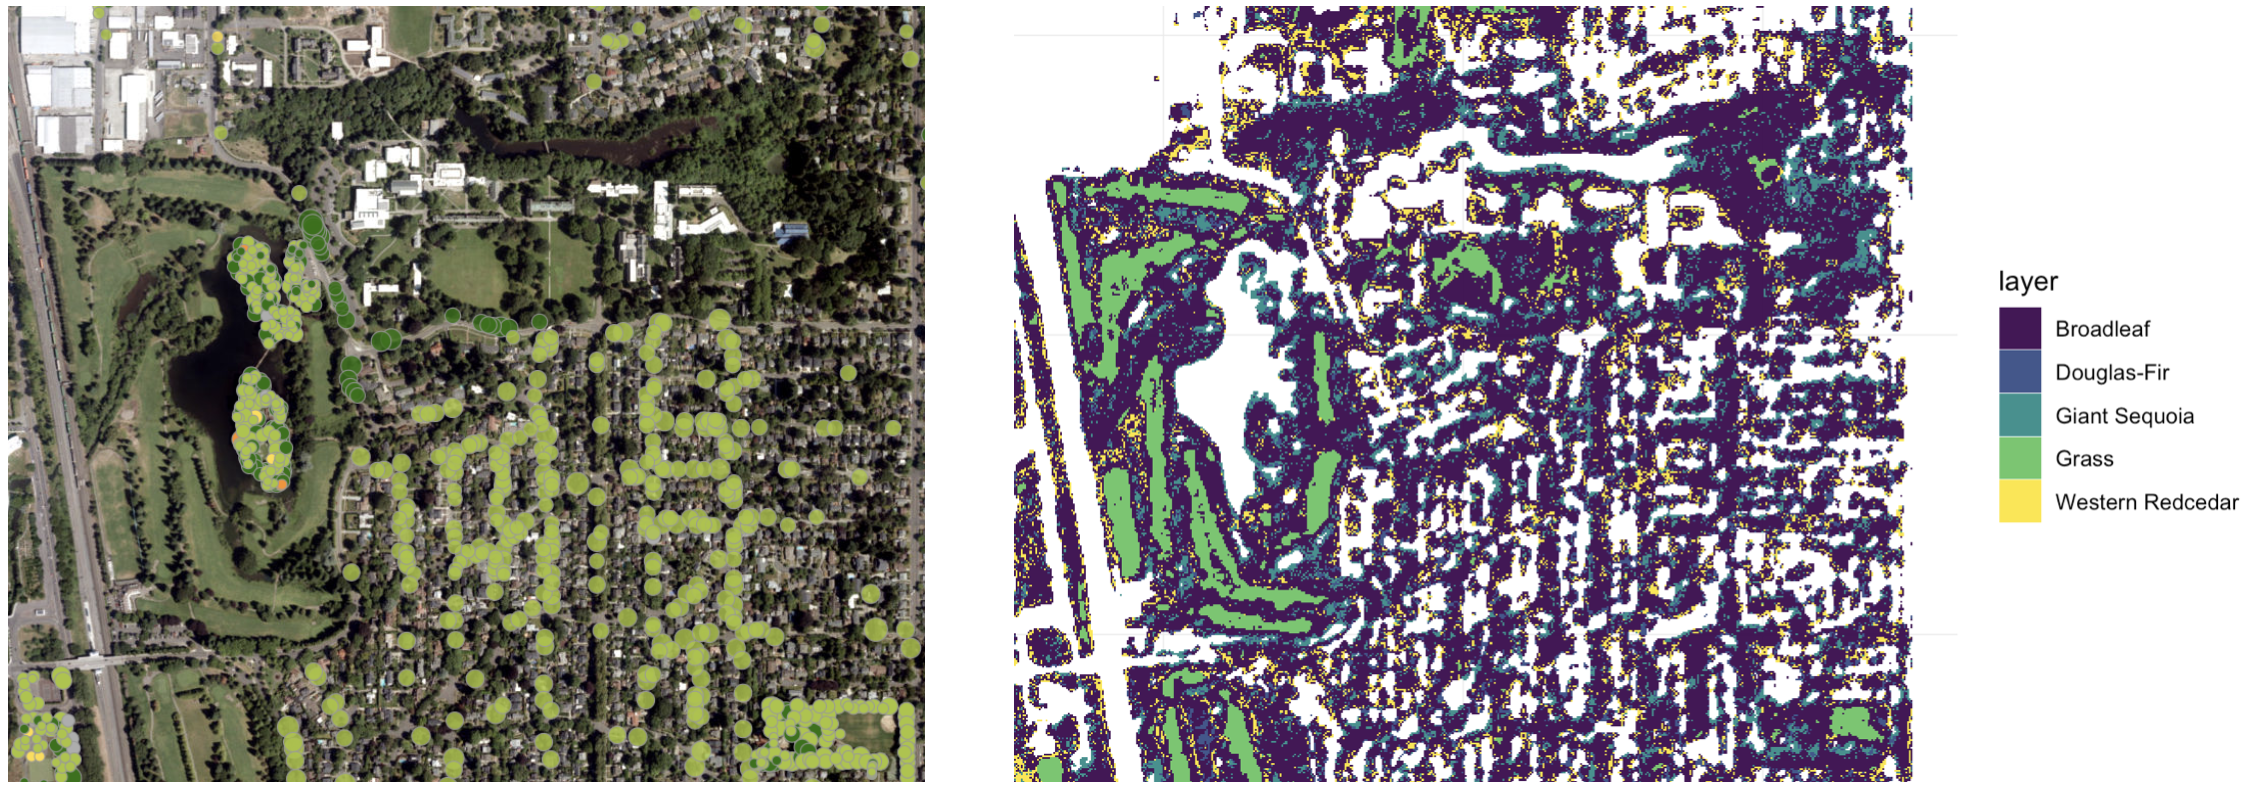
\includegraphics[width=1\linewidth]{figure/reedTreesTopdx} 

}

\caption{Comparison of tree model predictions (right) with pdxTrees (left) around Reed College. On the left, the circles mark the locations of pdxTrees, with color and shape indicating tree species and size according to the settings found on the website ('Tree Inventory Project'). On the right, the different colored pixels represent model predictions.}\label{fig:reedTreesTopdx}
\end{figure}
\hypertarget{discussion}{%
\chapter{Discussion}\label{discussion}}

\hypertarget{polygon-pixel-extraction-versus-point-pixel-extraction}{%
\section{Polygon Pixel Extraction Versus Point Pixel Extraction}\label{polygon-pixel-extraction-versus-point-pixel-extraction}}

Following along with the Fricker Methods (Fricker et al., 2019), a training dataset is constructed with multiple pixels from a single tree (extracted from the polygon shape). Another dataset was included in the methods of this research constructed with single pixels representing individual trees to investigate how the methods compare. Especially with low-resolution imagery, this analysis questions whether several pixels representing one tree in training a model is more beneficial than having a single pixel representing one tree (where that pixel is the center location of the tree's canopy). In terms of overall accuracies, the point pixel models did not perform as well as the pixel models. The most comparable Western Redcedar prediction accuracy among the point pixel models was the RF P = 8, C = 5 model, which was 0.29, which is low compared to the radial SVM C = 5 model on pixel data with 0.44 Western Redcedar accuracy, but close to the RF C = 7 models which predicted around 0.33 for Western Redcedars. The other point pixel models performed worse in overall validation accuracy, suggesting that polygon pixel extraction provides more information to train the model with more accuracy. One explanation for this discrepancy is that the field data from \texttt{pdxTrees} does not perfectly line up with tree locations on the satellite images, and this is especially true for smaller trees. Larger trees tend to have canopies that extend over the point pixel location, making up for the error in the point representing the tree's marked location. On the other hand, smaller trees (especially with canopies less than 3 meters across) are not centered around the point pixel, instead they tend to be about a pixel away. Extracting these pixel values is likely extracting the values of the street, sidewalk, shadow, grass, or other structure instead of the desired tree pixel. This analysis reveals how the model performance is sensitive to the training data going into the model, which emphasizes the importance of accurate field work. A potential improvement could be to relocate the point pixels so that they are perfectly centered over the tree canopies, however, this approach would be time-consuming.

\hypertarget{rf-performance-versus-svm-performance}{%
\section{RF Performance Versus SVM Performance}\label{rf-performance-versus-svm-performance}}

The 7 predictor RF model predicting 5 classes outperforms the SVM model predicting 5 classes in Western Redcedar training accuracy and testing overall accuracy as well as testing prediction of Western Redcedars. Surprisingly, the overall testing accuracies were higher than the validation accuracies for both the RF and SVM models. This suggests that the training set was not representative of the true data or the model was underfitting the data. The SVM model performs significantly worse than the RF model in Western Redcedar predictions on the test data. This could be a reflection of the fact that, by nature, SVM models perform poorly with data that have a lot of overlap and the pixel densities in Figure \ref{fig:pixDensity} appear to be similar, so observations will have overlap. One other explanation might be that the validation Western Redcedar accuracy aggregates the results of all 10 cross-validation sets, which inflates the values, but the test results only consists of one set. Another explanation could be that the lower testing accuracy is an indication of model overfitting, however, the overall testing accuracy is higher than the overall training accuracy. In general, having a small number of predictors compared to the number of classes tends to perform poorly. It was also observed that the models predicting less classes (Broadleaf, Douglas-Fir, Giant Sequoia, Grass, and Western Redcedar) outperformed models predicting on a larger set of tree classes (Bigleaf Maple, English Oak, Norway Maple, Douglas-Fir, Giant Sequoia, Grass, and Western Redcedar). This is likely a result of only having 4-band imagery plus the variables that are linear combinations of these 4 bands; 8 predictors training a model to predict 7 classes will not predict as well as 8 predictors training a model to predict 5 classes. In comparing the entire RF results on Portland to the \texttt{pdxTrees}, the test accuracy was 0.57. Since this is only using Western Redcedar trees from \texttt{pdxTrees}, the accuracy does not provide a true interpretation of how well the model performs on prediction locations and species for trees that were excluded from Portland's Inventory Project.

\hypertarget{model-results-compared-to-fricker-methods-fricker_convolutional_2019}{%
\section{Model Results Compared to Fricker Methods (Fricker et al., 2019)}\label{model-results-compared-to-fricker-methods-fricker_convolutional_2019}}

Fricker's methods are conducted under ideal circumstances. The single image strip used in the study had a spatial resolution of 1 meter, they had access to both hyperspectral imagery and RGB imagery, and the ground data was carefully collected to consist of seven tree species (Fricker et al., 2019). Fricker's results show that models using hyperspectral images performed better than RGB image models because they provide additional information by including spectral band combinations not available from RGB images. For this research, the images only consist of 4 bands (red, green, blue, and infrared), are accessible online, and have a spatial resolution of 3 meters. Upon closer inspection of the point data from \texttt{pdxTrees} on the satellite images, the pixels are not all properly aligned with the tree location. This is especially apparent with smaller tree canopies, where the pixel directly below the tree point often does not even overlap with the tree. This negatively impacts the point pixel results of the analysis, however, the polygon pixel results involved data that was carefully extracted to ensure the tree pixels are representative of a tree canopy, so it performed better. Unfortunately, the inconsistency of the point pixel locations impacts the interpretation of the testing results since the estimates for Western Redcedar locations are compared against the locations of the \texttt{pdxTrees} Western Redcedar locations. The resulting test accuracy is likely an underestimate. Fricker's methods applying a convolution neural network using hyperspectral imagery produced cross-validation training accuracies of 87\%. On just RGB imagery, this accuracy dropped to 64\%, which is a slight improvement over the best performing model (RF P = 7, C = 5) from this research which had a cross-validation training accuracy of 57\%. Across Portland, the (lower bound) testing accuracy of the RF P = 7, C = 5 model was 66\% for Western Redcedars.

\hypertarget{methods-of-improvementfurther-work}{%
\section{Methods of Improvement/Further Work}\label{methods-of-improvementfurther-work}}

Satellite imagery is widely applied to spatial data applications in environmental fields, and much of the research using remote sensing images has been published for classifying land type. Often this research is conducted under ideal circumstances with fine spatial and spectral resolution data, however, images at such a resolution usually require payment. This research applies imaging methods to satellite data with fewer bands and poorer resolution and investigates improvements to make up for the loss of resolution.

As Fricker's article has shown, increasing the spectral resolution by having access to hyperspectral data adds more information to the models and improves performance. Hyperspectral imagery collects information from more regions of the spectrum than RGB imagery, which allows it to capture more spectral features. Tree and vegetation pixels reflect a certain amount of light, especially regions of dense forests, so having more bands can allow the models to detect subtle differences in the spectral profile of different species. By increasing the number of variables in the model, the risk of multicollinearity that comes from artificially creating predictors with linear combinations of the RGB bands also gets removed. The benefits of high spatial and spectral resolution imagery also extends to improving the masks applied to the images, which were successful, for example, in removing building structures and dead fields of grass, but incorrectly recognized mossy lakes as trees. Carefully masking the images improves the ability of the model to locate tree pixels and classify them.

In terms of data, another improvement to this research would be to increase the spatial resolution to 1 meter or better if possible. This refines the process of creating polygons by enhancing the visibility of the tree canopy outlines and reduces noise in polygons introduced by having shadows, dirt, building structures, and other non-tree pixels and even within a single pixel. Another method to improve the results is by improving the drawn polygons themselves to only include pixels that represent the tree canopy. Drawing the polygons for each tree species by hand is likely to introduce error to the analysis because the first few polygons are not likely to be drawn the same way that the last few polygons are drawn. This issue is addressed by taking care to only include pure tree pixels (no shadows, dirt, or other structures) and ensuring that each polygon consists of at least 10 pixels.

An ideal training data set for the models would consist of data from imagery with high spatial and spectral resolution and also polygons with pure tree canopy pixels. If multiple raster strips are neccessary for the area of interest, the polygons need to be evenly distributed across all raster strips and ideally the tree species per polygon as well. The trees themselves should have large canopies that hopefully do not overlap with other tree canopies of different species.

With these improvements, the research will allow researchers to have a better understanding of the locations of redcedars in Portland. From there, this information provides a way to track future changes in redcedar trees's health, and inform decisions about tree management in the city. In a broader context, applying this method to Portland imagery data with multiple strips provides information about the applicability of modelling tree locations in different parts of the world and with data from different satellites. Ultimately, tracking the changes of the ecosystem allows people to take steps to preserve dying species.

\hypertarget{conclusion}{%
\section{Conclusion}\label{conclusion}}

Reports of Western Redcedars in the Pacific Northwest over the past 10 years have sparked an interest in investigating the decline of the species. This research combined RGB imagery and ground-level data available for the city of Portland to try and predict the locations of Western Redcedars and progress towards understanding the decline of the species and eventually expand the methods to larger regions like the Pacific Northwest. Ground-level data was used to locate individual tree canopies and label their species on the satellite images, then the light intensities were extracted for each tree canopy pixel into a training data set. Random forest and support vector machine models were trained to classify 7 or 5 tree species. The best performing model was the random forest model with 7 predictors on 5 tree species with an F-score of 0.27 for Western Redcedars. These results were not as high as other results from data with better conditions (higher spatial and spectral resolutions), however, they provide a better way of classifying a tree pixel as Western Redcedar than a random guess of one of the 7 species (probability of \(1/7 \approx 0.14\)).

The results of this research are replicable, since it involves data from open sources and the coding is completed in RStudio, and not too computationally intensive to require more than a day to run all of the code. Another key takeaway is that this research applies the methods of using remote sensing imagery to classify tree species in Portland specifically and provides a guideline for general areas to focus on locating Western Redcedars. The research is another application of remote sensing for tree species classification, which has the potential to predict more tree species in larger regions with more research.

\appendix

\hypertarget{tables}{%
\chapter{Tables}\label{tables}}

This appendix includes the cross-validation confusion matrices for all of the models on the training data and the confusion matrices on the testing data.

\ref{tab:cmsmallrf}
\begin{table}[!h]

\caption{\label{tab:cmsmallrf}RF Cross-Validation Confusion Matrix for P = 7, C = 7}
\centering
\resizebox{\linewidth}{!}{
\begin{tabular}[t]{l|r|r|r|r|r|r|r}
\hline
  & Bigleaf Maple & Douglas-Fir & English Oak & Giant Sequoia & grass & Norway Maple & Western Redcedar\\
\hline
Bigleaf Maple & 6.3714 & 0.8286 & 1.4857 & 1.7429 & 0.0571 & 3.3714 & 1.8286\\
\hline
Douglas-Fir & 0.9143 & 4.4571 & 1.8000 & 1.8571 & 0.0286 & 0.8857 & 2.2000\\
\hline
English Oak & 1.0286 & 2.8000 & 5.3143 & 2.2857 & 0.0000 & 1.1143 & 2.4571\\
\hline
Giant Sequoia & 1.4857 & 2.2000 & 2.1714 & 4.7429 & 0.0286 & 1.6000 & 1.2286\\
\hline
grass & 0.9429 & 0.0000 & 0.0286 & 0.1429 & 13.8286 & 1.0286 & 0.3429\\
\hline
Norway Maple & 2.4857 & 1.3714 & 0.9429 & 1.8571 & 0.2857 & 4.5429 & 1.6286\\
\hline
Western Redcedar & 1.0571 & 2.6286 & 2.5429 & 1.6571 & 0.0571 & 1.7429 & 4.6000\\
\hline
\end{tabular}}
\end{table}
\ref{tab:cmfullrf}
\begin{table}[!h]

\caption{\label{tab:cmfullrf}RF Cross-Validation Confusion Matrix for P = 8, C = 7}
\centering
\resizebox{\linewidth}{!}{
\begin{tabular}[t]{l|r|r|r|r|r|r|r}
\hline
  & Bigleaf Maple & Douglas-Fir & English Oak & Giant Sequoia & grass & Norway Maple & Western Redcedar\\
\hline
Bigleaf Maple & 6.4000 & 0.7143 & 1.6857 & 1.8571 & 0.1714 & 3.2000 & 1.6857\\
\hline
Douglas-Fir & 0.8857 & 4.8000 & 1.8857 & 1.5143 & 0.0286 & 1.2571 & 1.9143\\
\hline
English Oak & 0.9429 & 2.8571 & 5.4571 & 2.4000 & 0.0000 & 0.8857 & 2.5143\\
\hline
Giant Sequoia & 1.5429 & 2.2571 & 2.0000 & 4.8286 & 0.0000 & 1.6571 & 1.4000\\
\hline
grass & 0.8571 & 0.0000 & 0.0286 & 0.1429 & 13.6571 & 0.9143 & 0.3714\\
\hline
Norway Maple & 2.5429 & 1.1714 & 0.7143 & 1.9714 & 0.3429 & 4.7714 & 1.7143\\
\hline
Western Redcedar & 1.1143 & 2.4857 & 2.5143 & 1.5714 & 0.0857 & 1.6000 & 4.6857\\
\hline
\end{tabular}}
\end{table}
\ref{tab:cmcenterrf}
\begin{table}[!h]

\caption{\label{tab:cmcenterrf}RF Cross-Validation Confusion Matrix for P = 8, C = 5 (point)}
\centering
\resizebox{\linewidth}{!}{
\begin{tabular}[t]{l|r|r|r|r|r}
\hline
  & Bigleaf Maple & Douglas-Fir & Giant Sequoia & Norway Maple & Western Redcedar\\
\hline
Bigleaf Maple & 2.6346 & 4.4674 & 4.6964 & 3.7801 & 5.0401\\
\hline
Douglas-Fir & 4.8110 & 5.9565 & 3.4364 & 4.0092 & 2.9782\\
\hline
Giant Sequoia & 4.9255 & 2.7491 & 3.2073 & 4.5819 & 2.1764\\
\hline
Norway Maple & 2.9782 & 4.0092 & 3.5510 & 4.2383 & 3.4364\\
\hline
Western Redcedar & 4.6964 & 2.8637 & 4.9255 & 3.4364 & 6.4147\\
\hline
\end{tabular}}
\end{table}
\ref{tab:cmsmallgroupedrf}
\begin{table}[!h]

\caption{\label{tab:cmsmallgroupedrf}RF Cross-Validation Confusion Matrix for P = 7, C = 5}
\centering
\resizebox{\linewidth}{!}{
\begin{tabular}[t]{l|r|r|r|r|r}
\hline
  & Broadleaf & Douglas-Fir & Giant Sequoia & grass & Western Redcedar\\
\hline
Broadleaf & 33.2000 & 7.2000 & 8.7429 & 0.6000 & 9.0286\\
\hline
Douglas-Fir & 2.0571 & 4.1429 & 1.1143 & 0.0286 & 1.1714\\
\hline
Giant Sequoia & 2.8000 & 1.4571 & 3.3143 & 0.0000 & 0.6857\\
\hline
grass & 1.8286 & 0.0000 & 0.1143 & 13.6286 & 0.2857\\
\hline
Western Redcedar & 2.9714 & 1.4857 & 1.0000 & 0.0286 & 3.1143\\
\hline
\end{tabular}}
\end{table}
\ref{tab:cmfullgroupedrf}
\begin{table}[!h]

\caption{\label{tab:cmfullgroupedrf}RF Cross-Validation Confusion Matrix for P = 8, C = 5}
\centering
\resizebox{\linewidth}{!}{
\begin{tabular}[t]{l|r|r|r|r|r}
\hline
  & Broadleaf & Douglas-Fir & Giant Sequoia & grass & Western Redcedar\\
\hline
Broadleaf & 32.2000 & 6.6571 & 8.0857 & 0.8571 & 8.6000\\
\hline
Douglas-Fir & 2.3429 & 4.2857 & 1.4571 & 0.0286 & 1.3714\\
\hline
Giant Sequoia & 3.3714 & 1.6000 & 3.5429 & 0.0000 & 0.8000\\
\hline
grass & 1.6571 & 0.0000 & 0.1143 & 13.3714 & 0.2571\\
\hline
Western Redcedar & 3.2857 & 1.7429 & 1.0857 & 0.0286 & 3.2571\\
\hline
\end{tabular}}
\end{table}
\ref{tab:cmcentergroupedrf}
\begin{table}[!h]

\caption{\label{tab:cmcentergroupedrf}RF Cross-Validation Confusion Matrix for P = 8, C = 4 (point)}
\centering
\resizebox{\linewidth}{!}{
\begin{tabular}[t]{l|r|r|r|r}
\hline
  & Broadleaf & Douglas-Fir & Giant Sequoia & Western Redcedar\\
\hline
Broadleaf & 22.7950 & 13.6312 & 12.8293 & 12.3711\\
\hline
Douglas-Fir & 5.1546 & 3.2073 & 1.8328 & 2.2910\\
\hline
Giant Sequoia & 5.7274 & 1.4891 & 3.0928 & 1.9473\\
\hline
Western Redcedar & 6.4147 & 1.7182 & 2.0619 & 3.4364\\
\hline
\end{tabular}}
\end{table}
\ref{tab:scm1}
\begin{table}[!h]

\caption{\label{tab:scm1}Linear SVM Cross-Validation Confusion Matrix C = 7}
\centering
\resizebox{\linewidth}{!}{
\begin{tabular}[t]{l|r|r|r|r}
\hline
  & Broadleaf & Douglas-Fir & Giant Sequoia & Western Redcedar\\
\hline
Broadleaf & 40.0916 & 20.0458 & 19.8167 & 20.0458\\
\hline
Douglas-Fir & 0.0000 & 0.0000 & 0.0000 & 0.0000\\
\hline
Giant Sequoia & 0.0000 & 0.0000 & 0.0000 & 0.0000\\
\hline
Western Redcedar & 0.0000 & 0.0000 & 0.0000 & 0.0000\\
\hline
\end{tabular}}
\end{table}
\ref{tab:scm2}
\begin{table}[!h]

\caption{\label{tab:scm2}Radial SVM Cross-Validation Confusion Matrix C = 7}
\centering
\resizebox{\linewidth}{!}{
\begin{tabular}[t]{l|r|r|r|r|r|r|r}
\hline
  & Bigleaf Maple & Douglas-Fir & English Oak & Giant Sequoia & grass & Norway Maple & Western Redcedar\\
\hline
Bigleaf Maple & 7.1429 & 0.8000 & 1.6857 & 2.4286 & 0.0000 & 4.3429 & 2.2286\\
\hline
Douglas-Fir & 0.5714 & 3.6000 & 0.4857 & 0.2286 & 0.0000 & 0.1143 & 0.7143\\
\hline
English Oak & 0.6286 & 2.7714 & 5.0857 & 2.1429 & 0.0000 & 0.9143 & 2.0286\\
\hline
Giant Sequoia & 1.5143 & 3.1143 & 3.1429 & 5.9714 & 0.0000 & 1.8286 & 1.4000\\
\hline
grass & 1.3429 & 0.0000 & 0.0571 & 0.2286 & 14.0000 & 1.2571 & 0.4571\\
\hline
Norway Maple & 2.2000 & 1.0571 & 0.7714 & 1.3429 & 0.2857 & 3.8286 & 1.7429\\
\hline
Western Redcedar & 0.8857 & 2.9429 & 3.0571 & 1.9429 & 0.0000 & 2.0000 & 5.7143\\
\hline
\end{tabular}}
\end{table}
\ref{tab:scm3}
\begin{table}[!h]

\caption{\label{tab:scm3}Polynomial SVM Cross-Validation Confusion Matrix C = 7}
\centering
\resizebox{\linewidth}{!}{
\begin{tabular}[t]{l|r|r|r|r|r|r|r}
\hline
  & Bigleaf Maple & Douglas-Fir & English Oak & Giant Sequoia & grass & Norway Maple & Western Redcedar\\
\hline
Bigleaf Maple & 8.2000 & 1.4857 & 2.1714 & 3.1714 & 0.0286 & 5.4000 & 2.9429\\
\hline
Douglas-Fir & 0.4571 & 3.1714 & 0.4286 & 0.1143 & 0.0000 & 0.0857 & 0.4286\\
\hline
English Oak & 0.6000 & 2.9429 & 4.6571 & 1.9429 & 0.0000 & 0.8286 & 2.2286\\
\hline
Giant Sequoia & 1.2857 & 3.1429 & 3.3143 & 5.8857 & 0.0000 & 1.7714 & 1.3143\\
\hline
grass & 1.0857 & 0.0000 & 0.0286 & 0.1429 & 14.0000 & 1.2286 & 0.4286\\
\hline
Norway Maple & 1.7143 & 0.8000 & 0.6286 & 0.9429 & 0.2286 & 3.0857 & 1.4571\\
\hline
Western Redcedar & 0.9429 & 2.7429 & 3.0571 & 2.0857 & 0.0286 & 1.8857 & 5.4857\\
\hline
\end{tabular}}
\end{table}
\ref{tab:scm2grouped}
\begin{table}[!h]

\caption{\label{tab:scm2grouped}Radial SVM Cross-Validation Confusion Matrix C = 5}
\centering
\resizebox{\linewidth}{!}{
\begin{tabular}[t]{l|r|r|r|r|r}
\hline
  & Broadleaf & Douglas-Fir & Giant Sequoia & grass & Western Redcedar\\
\hline
Broadleaf & 37.7143 & 9.5143 & 11.4857 & 0.3714 & 11.8000\\
\hline
Douglas-Fir & 0.7429 & 3.0571 & 0.1143 & 0.0000 & 0.4286\\
\hline
Giant Sequoia & 1.0857 & 1.2571 & 2.3143 & 0.0000 & 0.1143\\
\hline
grass & 2.1429 & 0.0000 & 0.1143 & 13.9143 & 0.3429\\
\hline
Western Redcedar & 1.1714 & 0.4571 & 0.2571 & 0.0000 & 1.6000\\
\hline
\end{tabular}}
\end{table}
\ref{tab:scm3grouped}
\begin{table}[!h]

\caption{\label{tab:scm3grouped}Polynomial SVM Cross-Validation Confusion Matrix C = 5}
\centering
\resizebox{\linewidth}{!}{
\begin{tabular}[t]{l|r|r|r|r|r}
\hline
  & Broadleaf & Douglas-Fir & Giant Sequoia & grass & Western Redcedar\\
\hline
Broadleaf & 39.2286 & 10.9143 & 12.4000 & 0.4286 & 13.5714\\
\hline
Douglas-Fir & 0.7143 & 2.4571 & 0.0857 & 0.0000 & 0.2000\\
\hline
Giant Sequoia & 0.5714 & 0.8857 & 1.6857 & 0.0000 & 0.1429\\
\hline
grass & 2.1714 & 0.0000 & 0.1143 & 13.8571 & 0.3143\\
\hline
Western Redcedar & 0.1714 & 0.0286 & 0.0000 & 0.0000 & 0.0571\\
\hline
\end{tabular}}
\end{table}
\ref{tab:scm1center}
\begin{table}[!h]

\caption{\label{tab:scm1center}Linear SVM Cross-Validation Confusion Matrix C = 5 (point)}
\centering
\resizebox{\linewidth}{!}{
\begin{tabular}[t]{l|r|r|r|r|r}
\hline
  & Bigleaf Maple & Douglas-Fir & Giant Sequoia & Norway Maple & Western Redcedar\\
\hline
Bigleaf Maple & 1.4891 & 1.3746 & 1.6037 & 1.2600 & 2.4055\\
\hline
Douglas-Fir & 4.5819 & 7.3310 & 5.0401 & 5.3837 & 4.2383\\
\hline
Giant Sequoia & 10.6529 & 8.0183 & 10.3093 & 8.2474 & 9.2784\\
\hline
Norway Maple & 1.3746 & 1.3746 & 1.0309 & 1.8328 & 1.9473\\
\hline
Western Redcedar & 1.9473 & 1.9473 & 1.8328 & 3.3219 & 2.1764\\
\hline
\end{tabular}}
\end{table}
\ref{tab:scm2center}
\begin{table}[!h]

\caption{\label{tab:scm2center}Radial SVM Cross-Validation Confusion Matrix C = 5 (point)}
\centering
\resizebox{\linewidth}{!}{
\begin{tabular}[t]{l|r|r|r|r|r}
\hline
  & Bigleaf Maple & Douglas-Fir & Giant Sequoia & Norway Maple & Western Redcedar\\
\hline
Bigleaf Maple & 1.2600 & 2.2910 & 1.7182 & 1.7182 & 1.6037\\
\hline
Douglas-Fir & 5.3837 & 6.5292 & 4.1237 & 5.7274 & 4.1237\\
\hline
Giant Sequoia & 5.8419 & 3.8946 & 6.1856 & 4.9255 & 5.6128\\
\hline
Norway Maple & 2.1764 & 2.7491 & 3.2073 & 2.0619 & 3.4364\\
\hline
Western Redcedar & 5.3837 & 4.5819 & 4.5819 & 5.6128 & 5.2692\\
\hline
\end{tabular}}
\end{table}
\ref{tab:scm3center}
\begin{table}[!h]

\caption{\label{tab:scm3center}Polynomial SVM Cross-Validation Confusion Matrix C = 5 (point)}
\centering
\resizebox{\linewidth}{!}{
\begin{tabular}[t]{l|r|r|r|r|r}
\hline
  & Bigleaf Maple & Douglas-Fir & Giant Sequoia & Norway Maple & Western Redcedar\\
\hline
Bigleaf Maple & 2.0619 & 2.1764 & 2.8637 & 2.2910 & 2.6346\\
\hline
Douglas-Fir & 5.1546 & 7.5601 & 4.8110 & 5.9565 & 4.6964\\
\hline
Giant Sequoia & 9.3929 & 6.7583 & 9.3929 & 6.8729 & 8.4765\\
\hline
Norway Maple & 0.8018 & 1.0309 & 0.6873 & 1.3746 & 0.8018\\
\hline
Western Redcedar & 2.6346 & 2.5200 & 2.0619 & 3.5510 & 3.4364\\
\hline
\end{tabular}}
\end{table}
\ref{tab:scm2centergrouped}
\begin{table}[!h]

\caption{\label{tab:scm2centergrouped}Radial SVM Cross-Validation Confusion Matrix C = 4 (point)}
\centering
\resizebox{\linewidth}{!}{
\begin{tabular}[t]{l|r|r|r|r}
\hline
  & Broadleaf & Douglas-Fir & Giant Sequoia & Western Redcedar\\
\hline
Broadleaf & 39.0607 & 18.7858 & 19.7022 & 19.8167\\
\hline
Douglas-Fir & 0.9164 & 1.1455 & 0.1145 & 0.1145\\
\hline
Giant Sequoia & 0.0000 & 0.0000 & 0.0000 & 0.0000\\
\hline
Western Redcedar & 0.1145 & 0.1145 & 0.0000 & 0.1145\\
\hline
\end{tabular}}
\end{table}
\ref{tab:scm3centergrouped}
\begin{table}[!h]

\caption{\label{tab:scm3centergrouped}Polynomial SVM Cross-Validation Confusion Matrix C = 4 (point)}
\centering
\resizebox{\linewidth}{!}{
\begin{tabular}[t]{l|r|r|r|r}
\hline
  & Broadleaf & Douglas-Fir & Giant Sequoia & Western Redcedar\\
\hline
Broadleaf & 39.8625 & 19.2440 & 19.7022 & 19.8167\\
\hline
Douglas-Fir & 0.1145 & 0.8018 & 0.1145 & 0.2291\\
\hline
Giant Sequoia & 0.1145 & 0.0000 & 0.0000 & 0.0000\\
\hline
Western Redcedar & 0.0000 & 0.0000 & 0.0000 & 0.0000\\
\hline
\end{tabular}}
\end{table}
\ref{tab:cmtestrf}
\begin{table}[!h]

\caption{\label{tab:cmtestrf}RF Test Data Confusion Matrix for P = 7, C = 5}
\centering
\resizebox{\linewidth}{!}{
\begin{tabular}[t]{l|r|r|r|r|r|r|r|r|r|r|r}
\hline
  & Sensitivity & Specificity & Pos Pred Value & Neg Pred Value & Precision & Recall & F1 & Prevalence & Detection Rate & Detection Prevalence & Balanced Accuracy\\
\hline
Class: Broadleaf & 0.78 & 0.68 & 0.57 & 0.85 & 0.57 & 0.78 & 0.66 & 0.35 & 0.27 & 0.48 & 0.73\\
\hline
Class: Douglas-Fir & 0.32 & 0.96 & 0.52 & 0.92 & 0.52 & 0.32 & 0.40 & 0.11 & 0.04 & 0.07 & 0.64\\
\hline
Class: Giant Sequoia & 0.23 & 0.96 & 0.45 & 0.90 & 0.45 & 0.23 & 0.31 & 0.12 & 0.03 & 0.06 & 0.60\\
\hline
Class: grass & 0.95 & 0.96 & 0.92 & 0.98 & 0.92 & 0.95 & 0.93 & 0.31 & 0.29 & 0.32 & 0.95\\
\hline
Class: Western Redcedar & 0.22 & 0.95 & 0.35 & 0.91 & 0.35 & 0.22 & 0.27 & 0.11 & 0.02 & 0.07 & 0.58\\
\hline
\end{tabular}}
\end{table}
\ref{tab:cmtestsvm}
\begin{table}[!h]

\caption{\label{tab:cmtestsvm}SVM Test Data Confusion Matrix C = 5}
\centering
\resizebox{\linewidth}{!}{
\begin{tabular}[t]{l|r|r|r|r|r|r|r|r|r|r|r}
\hline
  & Sensitivity & Specificity & Pos Pred Value & Neg Pred Value & Precision & Recall & F1 & Prevalence & Detection Rate & Detection Prevalence & Balanced Accuracy\\
\hline
Class: Broadleaf & 0.87 & 0.58 & 0.53 & 0.90 & 0.53 & 0.87 & 0.66 & 0.35 & 0.31 & 0.58 & 0.73\\
\hline
Class: Douglas-Fir & 0.22 & 0.99 & 0.73 & 0.91 & 0.73 & 0.22 & 0.33 & 0.11 & 0.02 & 0.03 & 0.60\\
\hline
Class: Giant Sequoia & 0.15 & 0.98 & 0.50 & 0.90 & 0.50 & 0.15 & 0.23 & 0.12 & 0.02 & 0.04 & 0.57\\
\hline
Class: grass & 0.96 & 0.96 & 0.91 & 0.98 & 0.91 & 0.96 & 0.94 & 0.31 & 0.30 & 0.33 & 0.96\\
\hline
Class: Western Redcedar & 0.11 & 0.98 & 0.47 & 0.90 & 0.47 & 0.11 & 0.18 & 0.11 & 0.01 & 0.03 & 0.55\\
\hline
\end{tabular}}
\end{table}
\hypertarget{code}{%
\chapter{Code}\label{code}}

This appendix includes the workflow and all the R code for replicating this research. The sections are the titles of the RMarkdown documents to be run in order:
\begin{itemize}
\tightlist
\item
  tree\_canopy\_polygons.Rmd
\item
  geographic\_join.Rmd
\item
  train\_test\_split.Rmd
\item
  svm\_randomforest\_models.Rmd
\item
  model\_results\_analysis.Rmd
\item
  veg\_mask.Rmd
\item
  portland\_model.Rmd
\end{itemize}
\hypertarget{tree_canopy_polygons.rmd}{%
\section{tree\_canopy\_polygons.Rmd}\label{tree_canopy_polygons.rmd}}

First the rasters need to be downloaded from Planet.com by creating an account and selecting a date with clear weather and Portland's location. The following libraries and functions are necessary to be loaded into your workspace:
\begin{Shaded}
\begin{Highlighting}[]
\CommentTok{# libraries}
\KeywordTok{library}\NormalTok{(caret)}
\KeywordTok{library}\NormalTok{(doParallel)}
\KeywordTok{library}\NormalTok{(gridExtra)}
\KeywordTok{library}\NormalTok{(pdxTrees)}
\KeywordTok{library}\NormalTok{(raster)}
\KeywordTok{library}\NormalTok{(sf)}
\KeywordTok{library}\NormalTok{(sp)}
\KeywordTok{library}\NormalTok{(tidyverse)}
\KeywordTok{library}\NormalTok{(tigris)}

\CommentTok{# write shapefile function}
\NormalTok{species_shapefile <-}\StringTok{ }\ControlFlowTok{function}\NormalTok{(species, id)\{}
\NormalTok{  train <-}\StringTok{ }\NormalTok{pdxTrees_combined }\OperatorTok
\StringTok{  }\KeywordTok{filter}\NormalTok{(Species }\OperatorTok\StringTok{ }\NormalTok{species, Crown_Width_NS }\OperatorTok{>=}\StringTok{ }\DecValTok{20}\NormalTok{)}
  \KeywordTok{coordinates}\NormalTok{(train) =}\StringTok{ }\ErrorTok{~}\StringTok{ }\NormalTok{Longitude }\OperatorTok{+}\StringTok{ }\NormalTok{Latitude}
  \KeywordTok{proj4string}\NormalTok{(train)<-}\StringTok{ }\KeywordTok{CRS}\NormalTok{(}\StringTok{"+proj=longlat +datum=WGS84"}\NormalTok{)}
\NormalTok{  raster}\OperatorTok{::}\KeywordTok{shapefile}\NormalTok{(train, }\KeywordTok{paste0}\NormalTok{(id, }\StringTok{"_shapefile.shp"}\NormalTok{))}
\NormalTok{\}}

\CommentTok{# extract values and tidy function}
\NormalTok{names <-}\StringTok{ }\KeywordTok{c}\NormalTok{(}\StringTok{"ID"}\NormalTok{, }\StringTok{"red"}\NormalTok{, }\StringTok{"green"}\NormalTok{, }\StringTok{"blue"}\NormalTok{, }\StringTok{"ir"}\NormalTok{)}
\NormalTok{pixels_extraction <-}\StringTok{ }\ControlFlowTok{function}\NormalTok{(stack, poly_df, id) \{}
\NormalTok{  val <-}\StringTok{ }\NormalTok{raster}\OperatorTok{::}\KeywordTok{extract}\NormalTok{(stack, poly_df, }\DataTypeTok{df =} \OtherTok{TRUE}\NormalTok{)}
  \KeywordTok{colnames}\NormalTok{(val) <-}\StringTok{ }\NormalTok{names}
\NormalTok{  val <-}\StringTok{ }\KeywordTok{drop_na}\NormalTok{(val) }\OperatorTok
\StringTok{    }\KeywordTok{mutate}\NormalTok{(}\DataTypeTok{rstrip =}\NormalTok{ id)}
  \KeywordTok{return}\NormalTok{(val)}
\NormalTok{\}}

\CommentTok{# function to sample data}
\NormalTok{sampling_data <-}\StringTok{ }\ControlFlowTok{function}\NormalTok{(dat, ratio, n_pixels) \{}
\NormalTok{  dat_sampled <-}\StringTok{ }\NormalTok{dat }\OperatorTok
\StringTok{  }\KeywordTok{group_by}\NormalTok{(rstrip, Cmmn_Nm) }\OperatorTok
\StringTok{  }\KeywordTok{slice_sample}\NormalTok{(}\DataTypeTok{prop =}\NormalTok{ ratio) }\OperatorTok
\StringTok{  }\KeywordTok{ungroup}\NormalTok{() }\OperatorTok
\StringTok{  }\KeywordTok{group_by}\NormalTok{(Cmmn_Nm) }\OperatorTok
\StringTok{  }\KeywordTok{slice_sample}\NormalTok{(}\DataTypeTok{n =}\NormalTok{ n_pixels) }\CommentTok{# selects n pixels from each class}
  \KeywordTok{return}\NormalTok{(dat_sampled)}
\NormalTok{\}}

\CommentTok{# function to select columns from data}
\NormalTok{selecting_data <-}\StringTok{ }\ControlFlowTok{function}\NormalTok{(dat) \{}
\NormalTok{  dat_selected <-}\StringTok{ }\NormalTok{dat }\OperatorTok
\StringTok{  }\NormalTok{dplyr}\OperatorTok{::}\KeywordTok{select}\NormalTok{(red, green, blue, ir, ndvi, Cmmn_Nm, red_blue, red_green, }
\NormalTok{                blue_green)}
  \KeywordTok{return}\NormalTok{(dat_selected)}
\NormalTok{\}}

\CommentTok{# function to create grouped data}
\NormalTok{grouping_data <-}\StringTok{ }\ControlFlowTok{function}\NormalTok{(dat) \{}
\NormalTok{  dat_grouped <-}\StringTok{ }\NormalTok{dat }\OperatorTok
\StringTok{    }\KeywordTok{mutate}\NormalTok{(}\DataTypeTok{Cmmn_Nm =} \KeywordTok{case_when}\NormalTok{(}
\NormalTok{    Cmmn_Nm }\OperatorTok\StringTok{ }\KeywordTok{c}\NormalTok{(}\StringTok{"Bigleaf Maple"}\NormalTok{, }\StringTok{"English Oak"}\NormalTok{, }\StringTok{"Norway Maple"}\NormalTok{) }\OperatorTok{~}\StringTok{ "Broadleaf"}\NormalTok{,}
    \OtherTok{TRUE} \OperatorTok{~}\StringTok{ }\KeywordTok{as.character}\NormalTok{(Cmmn_Nm)}
\NormalTok{  ))}
  \KeywordTok{return}\NormalTok{(dat_grouped)}
\NormalTok{\}}

\CommentTok{# random forest function}
\NormalTok{training_rf <-}\StringTok{ }\ControlFlowTok{function}\NormalTok{(dat) \{}
\NormalTok{  model <-}\StringTok{ }\KeywordTok{train}\NormalTok{(Cmmn_Nm}\OperatorTok{~}\NormalTok{., }\DataTypeTok{data =}\NormalTok{ dat, }\DataTypeTok{method =} \StringTok{"rf"}\NormalTok{, }\DataTypeTok{trControl =}\NormalTok{ control)}
  \KeywordTok{return}\NormalTok{(model)}
\NormalTok{\}}

\CommentTok{# support vector machine function}
\NormalTok{training_svm <-}\StringTok{ }\ControlFlowTok{function}\NormalTok{(dat, method) \{}
\NormalTok{  model <-}\StringTok{ }\KeywordTok{train}\NormalTok{(Cmmn_Nm }\OperatorTok{~}\NormalTok{., }\DataTypeTok{data =}\NormalTok{ dat, }\DataTypeTok{method =}\NormalTok{ method, }
                 \DataTypeTok{trControl =}\NormalTok{ train_control,}
              \DataTypeTok{preProcess =} \KeywordTok{c}\NormalTok{(}\StringTok{"center"}\NormalTok{,}\StringTok{"scale"}\NormalTok{))}
  \KeywordTok{return}\NormalTok{(model)}
\NormalTok{\}}

\CommentTok{# prep rasters function}
\NormalTok{predRaster <-}\StringTok{ }\ControlFlowTok{function}\NormalTok{(stack) \{}
\NormalTok{  stack <-}\StringTok{ }\KeywordTok{stack}\NormalTok{(stack, ((stack[[}\DecValTok{4}\NormalTok{]] }\OperatorTok{-}\StringTok{ }\NormalTok{stack[[}\DecValTok{1}\NormalTok{]])}\OperatorTok{/}\NormalTok{(stack[[}\DecValTok{4}\NormalTok{]] }\OperatorTok{+}\StringTok{ }\NormalTok{stack[[}\DecValTok{1}\NormalTok{]])),}
\NormalTok{                 (stack[[}\DecValTok{1}\NormalTok{]]}\OperatorTok{/}\NormalTok{stack[[}\DecValTok{3}\NormalTok{]]), (stack[[}\DecValTok{4}\NormalTok{]]}\OperatorTok{/}\NormalTok{stack[[}\DecValTok{1}\NormalTok{]]),}
\NormalTok{                 (stack[[}\DecValTok{1}\NormalTok{]]}\OperatorTok{/}\NormalTok{stack[[}\DecValTok{2}\NormalTok{]]), (stack[[}\DecValTok{3}\NormalTok{]]}\OperatorTok{/}\NormalTok{stack[[}\DecValTok{2}\NormalTok{]]))}
  \KeywordTok{names}\NormalTok{(stack) <-}\StringTok{ }\KeywordTok{c}\NormalTok{(}\StringTok{"red"}\NormalTok{, }\StringTok{"green"}\NormalTok{, }\StringTok{"blue"}\NormalTok{, }\StringTok{"ir"}\NormalTok{, }\StringTok{"ndvi"}\NormalTok{, }\StringTok{"red_blue"}\NormalTok{, }
                    \StringTok{"ir_red"}\NormalTok{, }\StringTok{"red_green"}\NormalTok{, }\StringTok{"blue_green"}\NormalTok{)}
\NormalTok{  cl <-}\StringTok{ }\KeywordTok{makeCluster}\NormalTok{(}\DecValTok{3}\NormalTok{, }\DataTypeTok{type =} \StringTok{"FORK"}\NormalTok{)  }
  \KeywordTok{registerDoParallel}\NormalTok{(cl)  }
\NormalTok{  results_RF <-}\StringTok{ }\NormalTok{raster}\OperatorTok{::}\KeywordTok{predict}\NormalTok{(stack, rf_small_grouped, }\DataTypeTok{progress =} \StringTok{"text"}\NormalTok{)}
\NormalTok{  results_SVM <-}\StringTok{ }\NormalTok{raster}\OperatorTok{::}\KeywordTok{predict}\NormalTok{(stack, svm2_grouped, }\DataTypeTok{progress =} \StringTok{"text"}\NormalTok{)}
\NormalTok{  results <-}\StringTok{ }\KeywordTok{stack}\NormalTok{(results_RF, results_SVM)}
  \KeywordTok{stopCluster}\NormalTok{(cl)}
  \KeywordTok{return}\NormalTok{(results)}
\NormalTok{\}}
\end{Highlighting}
\end{Shaded}
This code creates shapefiles for six tree species from \texttt{pdxTrees}:
\begin{Shaded}
\begin{Highlighting}[]
\CommentTok{# load data}
\NormalTok{pdxTrees_parks <-}\StringTok{ }\KeywordTok{get_pdxTrees_parks}\NormalTok{()}
\NormalTok{pdxTrees_streets <-}\StringTok{ }\KeywordTok{get_pdxTrees_streets}\NormalTok{() }\CommentTok{# site width in ft., diameter in in.}
\NormalTok{pdxTrees_parks_filtered <-}\StringTok{ }\NormalTok{pdxTrees_parks }\OperatorTok
\StringTok{  }\KeywordTok{select}\NormalTok{(Longitude, Latitude, Genus, Species, Common_Name, Crown_Width_NS, }
\NormalTok{         Crown_Width_EW, Crown_Base_Height, Condition)}
\NormalTok{pdxTrees_streets_filtered <-}\StringTok{ }\NormalTok{pdxTrees_streets }\OperatorTok
\StringTok{  }\KeywordTok{select}\NormalTok{(Longitude, Latitude, Genus, Species, Common_Name, Site_Width, Condition)}

\NormalTok{pdxTrees_combined <-}\StringTok{ }\KeywordTok{full_join}\NormalTok{(pdxTrees_parks_filtered, pdxTrees_streets_filtered)}

\CommentTok{# species shapefiles}
\KeywordTok{species_shapefile}\NormalTok{(}\StringTok{"QURO"}\NormalTok{, }\StringTok{"quro"}\NormalTok{)}
\KeywordTok{species_shapefile}\NormalTok{(}\StringTok{"SEGI"}\NormalTok{, }\StringTok{"segi"}\NormalTok{)}
\KeywordTok{species_shapefile}\NormalTok{(}\StringTok{"ACPL"}\NormalTok{, }\StringTok{"acpl"}\NormalTok{)}
\KeywordTok{species_shapefile}\NormalTok{(}\StringTok{"PSME"}\NormalTok{, }\StringTok{"psme"}\NormalTok{)}
\KeywordTok{species_shapefile}\NormalTok{(}\StringTok{"ACMA"}\NormalTok{, }\StringTok{"acma"}\NormalTok{)}

\CommentTok{# Western redcedar shapefile}
\NormalTok{train_redcedar <-}\StringTok{ }\NormalTok{pdxTrees_combined }\OperatorTok
\StringTok{  }\KeywordTok{filter}\NormalTok{(Common_Name }\OperatorTok\StringTok{ "Western Redcedar"}\NormalTok{, Crown_Width_NS }\OperatorTok{>=}\StringTok{ }\DecValTok{20}\NormalTok{)}
\KeywordTok{coordinates}\NormalTok{(train_redcedar) =}\StringTok{ }\ErrorTok{~}\StringTok{ }\NormalTok{Longitude }\OperatorTok{+}\StringTok{ }\NormalTok{Latitude}
\KeywordTok{proj4string}\NormalTok{(train_redcedar)<-}\StringTok{ }\KeywordTok{CRS}\NormalTok{(}\StringTok{"+proj=longlat +datum=WGS84"}\NormalTok{)}
\NormalTok{raster}\OperatorTok{::}\KeywordTok{shapefile}\NormalTok{(train_redcedar, }\StringTok{"redcedar_shapefile.shp"}\NormalTok{)}
\end{Highlighting}
\end{Shaded}
\hypertarget{geographic_join.rmd}{%
\section{geographic\_join.Rmd}\label{geographic_join.rmd}}

Once the tree species shapefiles are created, they are imported into QGIS for manual polygons to be drawn around 100 of each tree species. Since the Planet.com imagery has a spatial resolution of 3 meters, the drawn polygons should try to contain around 10-20 pixels. The polygon layer is imported into RStudio for further analysis. To create the pixels data, the polygons are used to indicate the pixels that should be extracted. The point pixels data comes from filtering \texttt{pdxTrees}. The following code performs this geographic join of data:
\begin{Shaded}
\begin{Highlighting}[]
\CommentTok{# load polygon shapefiles}
\NormalTok{acpl <-}\StringTok{ }\KeywordTok{st_read}\NormalTok{(}\StringTok{"~/tree_canopy/acpl_polygon.shp"}\NormalTok{)}
\NormalTok{psme <-}\StringTok{ }\KeywordTok{st_read}\NormalTok{(}\StringTok{"~/tree_canopy/psme_polygon.shp"}\NormalTok{)}
\NormalTok{quru <-}\StringTok{ }\KeywordTok{st_read}\NormalTok{(}\StringTok{"~/tree_canopy/quru_polygon.shp"}\NormalTok{)}
\NormalTok{redcedar <-}\StringTok{ }\KeywordTok{st_read}\NormalTok{(}\StringTok{"~/tree_canopy/redwood_polygon.shp"}\NormalTok{)}
\NormalTok{segi <-}\StringTok{ }\KeywordTok{st_read}\NormalTok{(}\StringTok{"~/tree_canopy/segi_polygon.shp"}\NormalTok{)}
\NormalTok{acma <-}\StringTok{ }\KeywordTok{st_read}\NormalTok{(}\StringTok{"~/tree_canopy/acma_polygon.shp"}\NormalTok{)}
\NormalTok{grass <-}\StringTok{ }\KeywordTok{st_read}\NormalTok{(}\StringTok{"~/tree_canopy/grass_polygon.shp"}\NormalTok{)}

\CommentTok{# add polygon tree type column}
\NormalTok{acpl}\OperatorTok{$}\NormalTok{id_type <-}\StringTok{ "acpl"}
\NormalTok{psme}\OperatorTok{$}\NormalTok{id_type <-}\StringTok{ "psme"}
\NormalTok{quru}\OperatorTok{$}\NormalTok{id_type <-}\StringTok{ "quru"}
\NormalTok{redcedar}\OperatorTok{$}\NormalTok{id_type <-}\StringTok{ "redcedar"}
\NormalTok{segi}\OperatorTok{$}\NormalTok{id_type <-}\StringTok{ "segi"}
\NormalTok{acma}\OperatorTok{$}\NormalTok{id_type <-}\StringTok{ "acma"}
\NormalTok{grass}\OperatorTok{$}\NormalTok{id_type <-}\StringTok{ "grass"}

\CommentTok{# combine polygon shapefiles}
\NormalTok{combined_poly <-}\StringTok{ }\KeywordTok{rbind}\NormalTok{(acpl, psme, quru, redcedar, segi, acma, grass)}

\CommentTok{# create multipolygon object}
\NormalTok{multi_poly <-}\StringTok{ }\KeywordTok{st_multipolygon}\NormalTok{(combined_poly}\OperatorTok{$}\NormalTok{geometry)}

\CommentTok{# load point datasets}
\NormalTok{acpl_pts <-}\StringTok{ }\KeywordTok{st_read}\NormalTok{(}\StringTok{"~/tree_imaging/shapefiles/acpl_shapefile.shp"}\NormalTok{)}
\NormalTok{psme_pts <-}\StringTok{ }\KeywordTok{st_read}\NormalTok{(}\StringTok{"~/tree_imaging/shapefiles/psme_shapefile.shp"}\NormalTok{)}
\NormalTok{quru_pts <-}\StringTok{ }\KeywordTok{st_read}\NormalTok{(}\StringTok{"~/tree_imaging/shapefiles/quru_shapefile.shp"}\NormalTok{)}
\NormalTok{redcedar_pts <-}\StringTok{ }\KeywordTok{st_read}\NormalTok{(}\StringTok{"~/tree_imaging/shapefiles/redcedar_shapefile.shp"}\NormalTok{)}
\NormalTok{segi_pts <-}\StringTok{ }\KeywordTok{st_read}\NormalTok{(}\StringTok{"~/tree_imaging/shapefiles/segi_shapefile.shp"}\NormalTok{)}
\NormalTok{acma_pts <-}\StringTok{ }\KeywordTok{st_read}\NormalTok{(}\StringTok{"~/tree_imaging/shapefiles/acma_shapefile.shp"}\NormalTok{)}

\CommentTok{# combine point datasets}
\NormalTok{combined_pts <-}\StringTok{ }\KeywordTok{rbind}\NormalTok{(acpl_pts, psme_pts, quru_pts, redcedar_pts, segi_pts, }
\NormalTok{                      acma_pts)}

\CommentTok{# join combined points to combined polygons}
\NormalTok{poly_join <-}\StringTok{ }\KeywordTok{st_join}\NormalTok{(combined_poly, combined_pts, }\DataTypeTok{largest =}\NormalTok{ T)}

\CommentTok{# tidy polygon-point dataset}
\NormalTok{poly_join <-}\StringTok{ }\NormalTok{poly_join }\OperatorTok
\StringTok{  }\KeywordTok{mutate}\NormalTok{(}\DataTypeTok{id =} \KeywordTok{c}\NormalTok{(}\DecValTok{1}\OperatorTok{:}\KeywordTok{nrow}\NormalTok{(poly_join)))}

\CommentTok{# load raster layer object}
\NormalTok{stack_a <-}\StringTok{ }\KeywordTok{stack}\NormalTok{(}\StringTok{"planet/20200902_184428_1005_3B_AnalyticMS_clip.tif"}\NormalTok{)}
\NormalTok{stack_b <-}\StringTok{ }\KeywordTok{stack}\NormalTok{(}\StringTok{"planet/20200902_184429_1005_3B_AnalyticMS_clip.tif"}\NormalTok{)}
\NormalTok{stack_c <-}\StringTok{ }\KeywordTok{stack}\NormalTok{(}\StringTok{"planet/20200902_183008_24_1065_3B_AnalyticMS_clip.tif"}\NormalTok{)}
\NormalTok{stack_d <-}\StringTok{ }\KeywordTok{stack}\NormalTok{(}\StringTok{"planet/20200902_183006_18_1065_3B_AnalyticMS_clip.tif"}\NormalTok{)}
\NormalTok{stack_e <-}\StringTok{ }\KeywordTok{stack}\NormalTok{(}\StringTok{"planet/20200902_184430_1005_3B_AnalyticMS_clip.tif"}\NormalTok{)}

\CommentTok{# match raster project to polygons}
\NormalTok{raster_crs <-}\StringTok{ }\KeywordTok{CRS}\NormalTok{(}\KeywordTok{projection}\NormalTok{(stack_a))}
\NormalTok{poly_join_reprojected <-}\StringTok{ }\KeywordTok{spTransform}\NormalTok{(}\KeywordTok{as_Spatial}\NormalTok{(poly_join), raster_crs)}
\CommentTok{# saveRDS(poly_join_reprojected, "data/poly_join_reprojected.rds")}

\CommentTok{# extract pixel values from polygons into a dataframe}
\NormalTok{val_a <-}\StringTok{ }\KeywordTok{pixels_extraction}\NormalTok{(stack_a, poly_join_reprojected, }\StringTok{"a"}\NormalTok{)}
\NormalTok{val_b <-}\StringTok{ }\KeywordTok{pixels_extraction}\NormalTok{(stack_b, poly_join_reprojected, }\StringTok{"b"}\NormalTok{)}
\NormalTok{val_c <-}\StringTok{ }\KeywordTok{pixels_extraction}\NormalTok{(stack_c, poly_join_reprojected, }\StringTok{"c"}\NormalTok{)}
\NormalTok{val_d <-}\StringTok{ }\KeywordTok{pixels_extraction}\NormalTok{(stack_d, poly_join_reprojected, }\StringTok{"d"}\NormalTok{)}
\NormalTok{val_e <-}\StringTok{ }\KeywordTok{pixels_extraction}\NormalTok{(stack_e, poly_join_reprojected, }\StringTok{"e"}\NormalTok{)}

\CommentTok{# semi_join returns rows of x where it can find a match in y}
\NormalTok{val_combined <-}\StringTok{ }\KeywordTok{rbind}\NormalTok{(val_a, }\KeywordTok{anti_join}\NormalTok{(val_b, val_a, }\DataTypeTok{by =} \StringTok{"ID"}\NormalTok{))}
\NormalTok{val_combined <-}\StringTok{ }\KeywordTok{rbind}\NormalTok{(val_combined, }\KeywordTok{anti_join}\NormalTok{(val_c, val_combined, }\DataTypeTok{by =} \StringTok{"ID"}\NormalTok{))}
\NormalTok{val_combined <-}\StringTok{ }\KeywordTok{rbind}\NormalTok{(val_combined, }\KeywordTok{anti_join}\NormalTok{(val_d, val_combined, }\DataTypeTok{by =} \StringTok{"ID"}\NormalTok{))}
\NormalTok{val_combined <-}\StringTok{ }\KeywordTok{rbind}\NormalTok{(val_combined, }\KeywordTok{anti_join}\NormalTok{(val_e, val_combined, }\DataTypeTok{by =} \StringTok{"ID"}\NormalTok{))}

\CommentTok{# tidy pixel table}
\NormalTok{pixels_data <-}\KeywordTok{left_join}\NormalTok{(val_combined, poly_join_reprojected }\OperatorTok\StringTok{ }
\StringTok{                          }\KeywordTok{rename}\NormalTok{(}\DataTypeTok{ID =}\NormalTok{ id)) }\OperatorTok
\StringTok{  }\KeywordTok{mutate}\NormalTok{(}\DataTypeTok{ndvi =}\NormalTok{ (ir }\OperatorTok{-}\StringTok{ }\NormalTok{red)}\OperatorTok{/}\NormalTok{(ir }\OperatorTok{+}\StringTok{ }\NormalTok{red), }
         \DataTypeTok{Cmmn_Nm =} \KeywordTok{replace_na}\NormalTok{(}\KeywordTok{as.character}\NormalTok{(Cmmn_Nm), }\StringTok{"grass"}\NormalTok{),}
         \DataTypeTok{red_blue =}\NormalTok{ red}\OperatorTok{/}\NormalTok{blue,}
         \CommentTok{# ir_red = ir/red,}
         \DataTypeTok{red_green =}\NormalTok{ red}\OperatorTok{/}\NormalTok{green,}
         \DataTypeTok{blue_green =}\NormalTok{ blue}\OperatorTok{/}\NormalTok{green)}

\CommentTok{# load single pixel tree points}
\NormalTok{pdxTrees_parks <-}\StringTok{ }\KeywordTok{get_pdxTrees_parks}\NormalTok{()}
\NormalTok{pdxTrees_streets <-}\StringTok{ }\KeywordTok{get_pdxTrees_streets}\NormalTok{()}
\NormalTok{pdxTrees_combined <-}\StringTok{ }\KeywordTok{full_join}\NormalTok{(pdxTrees_parks, pdxTrees_streets)}
\NormalTok{trees_dat <-}\StringTok{ }\NormalTok{pdxTrees_combined }\OperatorTok
\StringTok{  }\NormalTok{dplyr}\OperatorTok{::}\KeywordTok{filter}\NormalTok{(Common_Name }\OperatorTok\StringTok{ "Western Redcedar"} \OperatorTok{|}\StringTok{ }
\StringTok{                  }\NormalTok{Species }\OperatorTok\StringTok{ }\KeywordTok{unique}\NormalTok{(pixels_data}\OperatorTok{$}\NormalTok{Species),}
\NormalTok{                DBH }\OperatorTok{>=}\StringTok{ }\DecValTok{15}\NormalTok{)}


\CommentTok{# convert to spatial points and reproject}
\KeywordTok{coordinates}\NormalTok{(trees_dat) <-}\StringTok{ }\ErrorTok{~}\StringTok{ }\NormalTok{Longitude }\OperatorTok{+}\StringTok{ }\NormalTok{Latitude}
\KeywordTok{proj4string}\NormalTok{(trees_dat)<-}\StringTok{ }\KeywordTok{CRS}\NormalTok{(}\StringTok{"+proj=longlat +datum=WGS84"}\NormalTok{)}
\NormalTok{trees_reprojected <-}\StringTok{ }\KeywordTok{spTransform}\NormalTok{(trees_dat, raster_crs)}

\CommentTok{# extract pixels for all trees}
\NormalTok{pix_a <-}\StringTok{ }\KeywordTok{pixels_extraction}\NormalTok{(stack_a, trees_reprojected, }\StringTok{"a"}\NormalTok{)}
\NormalTok{pix_b <-}\StringTok{ }\KeywordTok{pixels_extraction}\NormalTok{(stack_b, trees_reprojected, }\StringTok{"b"}\NormalTok{)}
\NormalTok{pix_c <-}\StringTok{ }\KeywordTok{pixels_extraction}\NormalTok{(stack_c, trees_reprojected, }\StringTok{"c"}\NormalTok{)}
\NormalTok{pix_d <-}\StringTok{ }\KeywordTok{pixels_extraction}\NormalTok{(stack_d, trees_reprojected, }\StringTok{"d"}\NormalTok{)}
\NormalTok{pix_e <-}\StringTok{ }\KeywordTok{pixels_extraction}\NormalTok{(stack_e, trees_reprojected, }\StringTok{"e"}\NormalTok{)}

\CommentTok{# semi_join returns rows of x where it can find a match in y}
\NormalTok{pix_combined <-}\StringTok{ }\KeywordTok{rbind}\NormalTok{(pix_a, }\KeywordTok{anti_join}\NormalTok{(pix_b, pix_a, }\DataTypeTok{by =} \StringTok{"ID"}\NormalTok{))}
\NormalTok{pix_combined <-}\StringTok{ }\KeywordTok{rbind}\NormalTok{(pix_combined, }\KeywordTok{anti_join}\NormalTok{(pix_c, pix_combined, }\DataTypeTok{by =} \StringTok{"ID"}\NormalTok{))}
\NormalTok{pix_combined <-}\StringTok{ }\KeywordTok{rbind}\NormalTok{(pix_combined, }\KeywordTok{anti_join}\NormalTok{(pix_d, pix_combined, }\DataTypeTok{by =} \StringTok{"ID"}\NormalTok{))}
\NormalTok{pix_combined <-}\StringTok{ }\KeywordTok{rbind}\NormalTok{(pix_combined, }\KeywordTok{anti_join}\NormalTok{(pix_e, pix_combined, }\DataTypeTok{by =} \StringTok{"ID"}\NormalTok{))}

\CommentTok{# tidy centers pixel table}
\NormalTok{pix_tree_center <-}\StringTok{ }\NormalTok{pix_combined }\OperatorTok
\StringTok{  }\KeywordTok{mutate}\NormalTok{(}\DataTypeTok{ID =} \KeywordTok{as.character}\NormalTok{(ID)) }\OperatorTok
\StringTok{  }\KeywordTok{left_join}\NormalTok{(trees_reprojected}\OperatorTok{@}\NormalTok{data, }\DataTypeTok{by =} \KeywordTok{c}\NormalTok{(}\StringTok{"ID"}\NormalTok{ =}\StringTok{ "UserID"}\NormalTok{)) }\OperatorTok
\StringTok{  }\KeywordTok{mutate}\NormalTok{(}\DataTypeTok{ndvi =}\NormalTok{ (ir }\OperatorTok{-}\StringTok{ }\NormalTok{red)}\OperatorTok{/}\NormalTok{(ir }\OperatorTok{+}\StringTok{ }\NormalTok{red),}
         \DataTypeTok{red_blue =}\NormalTok{ red}\OperatorTok{/}\NormalTok{blue,}
         \CommentTok{# ir_red = ir/red,}
         \DataTypeTok{red_green =}\NormalTok{ red}\OperatorTok{/}\NormalTok{green,}
         \DataTypeTok{blue_green =}\NormalTok{ blue}\OperatorTok{/}\NormalTok{green,}
         \DataTypeTok{Cmmn_Nm =} \KeywordTok{case_when}\NormalTok{(}
\NormalTok{           Common_Name }\OperatorTok\StringTok{ "Maple, Norway"} \OperatorTok{~}\StringTok{ "Norway Maple"}\NormalTok{,}
\NormalTok{           Common_Name }\OperatorTok\StringTok{ "Maple, Bigleaf"} \OperatorTok{~}\StringTok{ "Bigleaf Maple"}\NormalTok{,}
           \OtherTok{TRUE} \OperatorTok{~}\StringTok{ }\KeywordTok{as.character}\NormalTok{(Common_Name)}
\NormalTok{         )) }\OperatorTok
\StringTok{  }\NormalTok{dplyr}\OperatorTok{::}\KeywordTok{filter}\NormalTok{(Cmmn_Nm }\OperatorTok\StringTok{ }\KeywordTok{c}\NormalTok{(}\StringTok{"Western Redcedar"}\NormalTok{, }\StringTok{"Bigleaf Maple"}\NormalTok{, }
                               \StringTok{"Douglas-Fir"}\NormalTok{, }\CommentTok{#"English Oak",}
                               \StringTok{"Giant Sequoia"}\NormalTok{, }\StringTok{"Norway Maple"}\NormalTok{))}

\CommentTok{# save results}
\CommentTok{# write.csv(poly_join_reprojected,'data/poly_join_reprojected1.csv', row.names = F)}
\CommentTok{# write.csv(val_combined,'data/val_combined1.csv', row.names = F)}
\CommentTok{# write.csv(pixels_data,'data/pixels_data.csv', row.names = F)}
\CommentTok{# write.csv(pix_tree_center,'data/pix_tree_center.csv', row.names = F)}
\end{Highlighting}
\end{Shaded}
\hypertarget{train_test_split.rmd}{%
\section{train\_test\_split.Rmd}\label{train_test_split.rmd}}

To prepare the data for training and testing the models, the pixels and point pixels data are split into training and testing data:
\begin{Shaded}
\begin{Highlighting}[]
\CommentTok{# load data}
\NormalTok{pixels_data <-}\StringTok{ }\KeywordTok{read.csv}\NormalTok{(}\StringTok{'data/pixels_data.csv'}\NormalTok{)}
\NormalTok{pix_tree_center <-}\StringTok{ }\KeywordTok{read.csv}\NormalTok{(}\StringTok{'data/pix_tree_center.csv'}\NormalTok{)}

\CommentTok{# take note of distribution of classes}
\NormalTok{pixels_data }\OperatorTok
\StringTok{  }\KeywordTok{count}\NormalTok{(Cmmn_Nm)}
\NormalTok{pix_tree_center }\OperatorTok
\StringTok{  }\KeywordTok{count}\NormalTok{(Cmmn_Nm)}

\CommentTok{# training data}
\KeywordTok{set.seed}\NormalTok{(}\DecValTok{2}\NormalTok{)}
\NormalTok{train_full <-}\StringTok{ }\KeywordTok{sampling_data}\NormalTok{(pixels_data, }\FloatTok{0.7}\NormalTok{, }\DecValTok{500}\NormalTok{)}
\NormalTok{train <-}\StringTok{ }\KeywordTok{selecting_data}\NormalTok{(train_full)}
\NormalTok{train_grouped <-}\StringTok{ }\KeywordTok{grouping_data}\NormalTok{(train)}
\NormalTok{train_center <-}\StringTok{ }\KeywordTok{selecting_data}\NormalTok{(}\KeywordTok{sampling_data}\NormalTok{(pix_tree_center, }\FloatTok{0.7}\NormalTok{, }\DecValTok{175}\NormalTok{))}
\NormalTok{train_center_grouped <-}\StringTok{ }\KeywordTok{grouping_data}\NormalTok{(train_center)}

\CommentTok{# testing data}
\NormalTok{test_full <-}\StringTok{ }\KeywordTok{anti_join}\NormalTok{(pixels_data, train_full)}
\NormalTok{test_full_grouped <-}\StringTok{ }\KeywordTok{grouping_data}\NormalTok{(test_full)}
\NormalTok{test <-}\StringTok{ }\NormalTok{test_full }\OperatorTok
\StringTok{  }\NormalTok{dplyr}\OperatorTok{::}\KeywordTok{select}\NormalTok{(red, green, blue, ir, ndvi, Cmmn_Nm, red_blue, red_green, }
\NormalTok{                blue_green)}
\NormalTok{test_grouped <-}\StringTok{ }\KeywordTok{grouping_data}\NormalTok{(test)}
\NormalTok{test_center <-}\StringTok{ }\KeywordTok{anti_join}\NormalTok{(pix_tree_center, train_center) }\OperatorTok
\StringTok{  }\NormalTok{dplyr}\OperatorTok{::}\KeywordTok{select}\NormalTok{(red, green, blue, ir, ndvi, Cmmn_Nm, red_blue, red_green, }
\NormalTok{                blue_green)}
\NormalTok{test_center_grouped <-}\StringTok{ }\KeywordTok{grouping_data}\NormalTok{(test_center)}

\CommentTok{# save results}
\CommentTok{# write.csv(train,'data/train.csv', row.names = F)}
\CommentTok{# write.csv(train_grouped,'data/train_grouped.csv', row.names = F)}
\CommentTok{# write.csv(train_center,'data/train_center.csv', row.names = F)}
\CommentTok{# write.csv(train_center_grouped,'data/train_center_grouped.csv', row.names = F)}
\CommentTok{# write.csv(test,'data/test.csv', row.names = F)}
\CommentTok{# write.csv(test_grouped,'data/test_grouped.csv', row.names = F)}
\CommentTok{# write.csv(test_center,'data/test_center.csv', row.names = F)}
\CommentTok{# write.csv(test_center_grouped,'data/test_center_grouped.csv', row.names = F)}
\CommentTok{# write.csv(test_full, 'data/test_full.csv', row.names = F)}
\CommentTok{# write.csv(test_full_grouped, 'data/test_full_grouped.csv', row.names = F)}
\end{Highlighting}
\end{Shaded}
\hypertarget{svm_randomforest_models.rmd}{%
\section{svm\_randomforest\_models.Rmd}\label{svm_randomforest_models.rmd}}

The training data is used to train the models:
\begin{Shaded}
\begin{Highlighting}[]
\CommentTok{# load training data}
\NormalTok{train <-}\StringTok{ }\KeywordTok{read.csv}\NormalTok{(}\StringTok{'data/train.csv'}\NormalTok{)}
\NormalTok{train_grouped <-}\StringTok{ }\KeywordTok{read.csv}\NormalTok{(}\StringTok{'data/train_grouped.csv'}\NormalTok{)}
\NormalTok{train_center <-}\StringTok{ }\KeywordTok{read.csv}\NormalTok{(}\StringTok{'data/train_center.csv'}\NormalTok{)}
\NormalTok{train_center_grouped <-}\StringTok{ }\KeywordTok{read.csv}\NormalTok{(}\StringTok{'data/train_center_grouped.csv'}\NormalTok{)}

\CommentTok{# random search random forest using caret package}
\NormalTok{control <-}\StringTok{ }\KeywordTok{trainControl}\NormalTok{(}\DataTypeTok{method =} \StringTok{"repeatedcv"}\NormalTok{, }\DataTypeTok{number =} \DecValTok{10}\NormalTok{, }
                        \DataTypeTok{search =} \StringTok{"random"}\NormalTok{)}

\KeywordTok{set.seed}\NormalTok{(}\DecValTok{2}\NormalTok{)}
\NormalTok{rf_small <-}\StringTok{ }\KeywordTok{training_rf}\NormalTok{(train }\OperatorTok\StringTok{ }\NormalTok{dplyr}\OperatorTok{::}\KeywordTok{select}\NormalTok{(}\OperatorTok{-}\KeywordTok{c}\NormalTok{(red_blue)))}
\NormalTok{rf_small_grouped <-}\StringTok{ }\KeywordTok{training_rf}\NormalTok{(train_grouped }\OperatorTok\StringTok{ }\NormalTok{dplyr}\OperatorTok{::}\KeywordTok{select}\NormalTok{(}\OperatorTok{-}\KeywordTok{c}\NormalTok{(red_blue)))}
\NormalTok{rf_full <-}\StringTok{ }\KeywordTok{training_rf}\NormalTok{(train)}
\NormalTok{rf_full_grouped <-}\StringTok{ }\KeywordTok{training_rf}\NormalTok{(train_grouped)}
\NormalTok{rf_center <-}\StringTok{ }\KeywordTok{training_rf}\NormalTok{(train_center)}
\NormalTok{rf_center_grouped <-}\StringTok{ }\KeywordTok{training_rf}\NormalTok{(train_center_grouped)}

\CommentTok{# 10 fold cross validation}
\NormalTok{train_control <-}\StringTok{ }\KeywordTok{trainControl}\NormalTok{(}\DataTypeTok{method =} \StringTok{"cv"}\NormalTok{, }\DataTypeTok{number =} \DecValTok{10}\NormalTok{)}

\KeywordTok{set.seed}\NormalTok{(}\DecValTok{2}\NormalTok{)}
\CommentTok{# fit svm model with normalized variables}
\NormalTok{svm1 <-}\StringTok{ }\KeywordTok{training_svm}\NormalTok{(train, }\StringTok{"svmLinear"}\NormalTok{)}
\NormalTok{svm2 <-}\StringTok{ }\KeywordTok{training_svm}\NormalTok{(train, }\StringTok{"svmRadial"}\NormalTok{)}
\NormalTok{svm3 <-}\StringTok{ }\KeywordTok{training_svm}\NormalTok{(train, }\StringTok{"svmPoly"}\NormalTok{)}
\NormalTok{svm1_grouped <-}\StringTok{ }\KeywordTok{training_svm}\NormalTok{(train_grouped, }\StringTok{"svmLinear"}\NormalTok{)}
\NormalTok{svm2_grouped <-}\StringTok{ }\KeywordTok{training_svm}\NormalTok{(train_grouped, }\StringTok{"svmRadial"}\NormalTok{)}
\NormalTok{svm3_grouped <-}\StringTok{ }\KeywordTok{training_svm}\NormalTok{(train_grouped, }\StringTok{"svmPoly"}\NormalTok{)}
\NormalTok{svm1_center <-}\StringTok{ }\KeywordTok{training_svm}\NormalTok{(train_center, }\StringTok{"svmLinear"}\NormalTok{)}
\NormalTok{svm2_center <-}\StringTok{ }\KeywordTok{training_svm}\NormalTok{(train_center, }\StringTok{"svmRadial"}\NormalTok{)}
\NormalTok{svm3_center <-}\StringTok{ }\KeywordTok{training_svm}\NormalTok{(train_center, }\StringTok{"svmPoly"}\NormalTok{)}
\NormalTok{svm1_center_grouped <-}\StringTok{ }\KeywordTok{training_svm}\NormalTok{(train_center_grouped, }\StringTok{"svmLinear"}\NormalTok{)}
\NormalTok{svm2_center_grouped <-}\StringTok{ }\KeywordTok{training_svm}\NormalTok{(train_center_grouped, }\StringTok{"svmRadial"}\NormalTok{)}
\NormalTok{svm3_center_grouped <-}\StringTok{ }\KeywordTok{training_svm}\NormalTok{(train_center_grouped, }\StringTok{"svmPoly"}\NormalTok{)}

\CommentTok{# save models}
\CommentTok{# saveRDS(rf_small, "data/rf_small.rds")}
\CommentTok{# saveRDS(rf_small_grouped, "data/rf_small_grouped.rds")}
\CommentTok{# saveRDS(rf_full, "data/rf_full.rds")}
\CommentTok{# saveRDS(rf_full_grouped, "data/rf_full_grouped.rds")}
\CommentTok{# saveRDS(rf_center, "data/rf_center.rds")}
\CommentTok{# saveRDS(rf_center_grouped, "data/rf_center_grouped.rds")}
\CommentTok{# saveRDS(svm1, "data/svm1.rds")}
\CommentTok{# saveRDS(svm2, "data/svm2.rds")}
\CommentTok{# saveRDS(svm3, "data/svm3.rds")}
\CommentTok{# saveRDS(svm1_center, "data/svm1_center.rds")}
\CommentTok{# saveRDS(svm2_center, "data/svm2_center.rds")}
\CommentTok{# saveRDS(svm3_center, "data/svm3_center.rds")}
\CommentTok{# saveRDS(svm1_grouped, "data/svm1_grouped.rds")}
\CommentTok{# saveRDS(svm2_grouped, "data/svm2_grouped.rds")}
\CommentTok{# saveRDS(svm3_grouped, "data/svm3_grouped.rds")}
\end{Highlighting}
\end{Shaded}
\hypertarget{model_results_analysis.rmd}{%
\section{model\_results\_analysis.Rmd}\label{model_results_analysis.rmd}}

Analysis on the trained models included in this research is conducted with the following code:
\begin{Shaded}
\begin{Highlighting}[]
\CommentTok{# load rf models}
\NormalTok{rf_small <-}\StringTok{ }\KeywordTok{readRDS}\NormalTok{(}\StringTok{"data/rf_small.rds"}\NormalTok{)}
\NormalTok{rf_small_grouped <-}\StringTok{ }\KeywordTok{readRDS}\NormalTok{(}\StringTok{"data/rf_small_grouped.rds"}\NormalTok{)}
\NormalTok{rf_full <-}\StringTok{ }\KeywordTok{readRDS}\NormalTok{(}\StringTok{"data/rf_full.rds"}\NormalTok{)}
\NormalTok{rf_full_grouped <-}\StringTok{ }\KeywordTok{readRDS}\NormalTok{(}\StringTok{"data/rf_full_grouped.rds"}\NormalTok{)}
\NormalTok{rf_center <-}\StringTok{ }\KeywordTok{readRDS}\NormalTok{(}\StringTok{"data/rf_center.rds"}\NormalTok{)}
\NormalTok{rf_center_grouped <-}\StringTok{ }\KeywordTok{readRDS}\NormalTok{(}\StringTok{"data/rf_center_grouped.rds"}\NormalTok{)}

\CommentTok{# rf mtry cross validation}
\KeywordTok{grid.arrange}\NormalTok{(}\KeywordTok{plot}\NormalTok{(rf_small, }\DataTypeTok{main =} \StringTok{"RF P = 7, C = 7"}\NormalTok{),}
             \KeywordTok{plot}\NormalTok{(rf_small_grouped, }\DataTypeTok{main =} \StringTok{"RF P = 7, C = 5"}\NormalTok{), }\DataTypeTok{nrow =} \DecValTok{1}\NormalTok{)}
\KeywordTok{grid.arrange}\NormalTok{(}\KeywordTok{plot}\NormalTok{(rf_full, }\DataTypeTok{main =} \StringTok{"RF P = 8, C = 7"}\NormalTok{),}
             \KeywordTok{plot}\NormalTok{(rf_full_grouped, }\DataTypeTok{main =} \StringTok{"RF P = 8, C = 5"}\NormalTok{), }\DataTypeTok{nrow =} \DecValTok{1}\NormalTok{)}
\KeywordTok{grid.arrange}\NormalTok{(}\KeywordTok{plot}\NormalTok{(rf_center, }\DataTypeTok{main =} \StringTok{"RF P = 8, C = 5 (point)"}\NormalTok{),}
             \KeywordTok{plot}\NormalTok{(rf_center_grouped, }\DataTypeTok{main =} \StringTok{"RF P = 8, C = 4 (point)"}\NormalTok{), }
             \DataTypeTok{nrow =} \DecValTok{1}\NormalTok{)}

\CommentTok{# data frame to compare rf models}
\NormalTok{results <-}\StringTok{ }\KeywordTok{rbind}\NormalTok{(}\KeywordTok{cbind}\NormalTok{(rf_small}\OperatorTok{$}\NormalTok{resample, }\DataTypeTok{Model =} \KeywordTok{rep}\NormalTok{(}\StringTok{"P = 7, C = 7"}\NormalTok{, }\DecValTok{10}\NormalTok{)), }
                 \KeywordTok{cbind}\NormalTok{(rf_full}\OperatorTok{$}\NormalTok{resample, }\DataTypeTok{Model =} \KeywordTok{rep}\NormalTok{(}\StringTok{"P = 8, C = 7"}\NormalTok{, }\DecValTok{10}\NormalTok{)),}
                 \KeywordTok{cbind}\NormalTok{(rf_center}\OperatorTok{$}\NormalTok{resample, }
                       \DataTypeTok{Model =} \KeywordTok{rep}\NormalTok{(}\StringTok{"P = 8, C = 5 (point)"}\NormalTok{, }\DecValTok{10}\NormalTok{)),}
                 \KeywordTok{cbind}\NormalTok{(rf_small_grouped}\OperatorTok{$}\NormalTok{resample, }
                       \DataTypeTok{Model =} \KeywordTok{rep}\NormalTok{(}\StringTok{"P = 7, C = 5"}\NormalTok{, }\DecValTok{10}\NormalTok{)),}
                 \KeywordTok{cbind}\NormalTok{(rf_full_grouped}\OperatorTok{$}\NormalTok{resample, }
                       \DataTypeTok{Model =} \KeywordTok{rep}\NormalTok{(}\StringTok{"P = 8, C = 5"}\NormalTok{, }\DecValTok{10}\NormalTok{)),}
                 \KeywordTok{cbind}\NormalTok{(rf_center_grouped}\OperatorTok{$}\NormalTok{resample, }
                       \DataTypeTok{Model =} \KeywordTok{rep}\NormalTok{(}\StringTok{"P = 8, C = 4 (point)"}\NormalTok{, }\DecValTok{10}\NormalTok{)))}

\CommentTok{# visualize rf model results}
\KeywordTok{ggplot}\NormalTok{(results, }\KeywordTok{aes}\NormalTok{(}\DataTypeTok{x =}\NormalTok{ Model, }\DataTypeTok{y =}\NormalTok{ Accuracy, }\DataTypeTok{fill =}\NormalTok{ Model)) }\OperatorTok{+}
\StringTok{  }\KeywordTok{geom_boxplot}\NormalTok{(}\DataTypeTok{alpha =} \FloatTok{0.6}\NormalTok{) }\OperatorTok{+}
\StringTok{  }\KeywordTok{theme_minimal}\NormalTok{() }\OperatorTok{+}\StringTok{ }
\StringTok{  }\KeywordTok{scale_fill_viridis_d}\NormalTok{() }\OperatorTok{+}
\StringTok{  }\KeywordTok{labs}\NormalTok{(}\DataTypeTok{title =} \StringTok{"Model Accuracy of Random Forest Models with 10-Fold CV"}\NormalTok{, }
       \DataTypeTok{x =} \StringTok{" "}\NormalTok{, }\DataTypeTok{fill =} \StringTok{"P = Predictors, C = Classes"}\NormalTok{) }\OperatorTok{+}\StringTok{ }
\StringTok{  }\KeywordTok{theme}\NormalTok{(}\DataTypeTok{axis.text.x =} \KeywordTok{element_blank}\NormalTok{())}

\CommentTok{# rf results by class}
\NormalTok{cm_small_rf <-}\StringTok{ }\KeywordTok{confusionMatrix}\NormalTok{(rf_small,  }\DataTypeTok{mode =} \StringTok{"prec_recall"}\NormalTok{)}
\NormalTok{cm_full_rf <-}\StringTok{ }\KeywordTok{confusionMatrix}\NormalTok{(rf_full,  }\DataTypeTok{mode =} \StringTok{"prec_recall"}\NormalTok{)}
\NormalTok{cm_center_rf <-}\StringTok{ }\KeywordTok{confusionMatrix}\NormalTok{(rf_center,  }\DataTypeTok{mode =} \StringTok{"prec_recall"}\NormalTok{)}
\NormalTok{cm_small_grouped_rf <-}\StringTok{ }\KeywordTok{confusionMatrix}\NormalTok{(rf_small_grouped,  }\DataTypeTok{mode =} \StringTok{"prec_recall"}\NormalTok{)}
\NormalTok{cm_full_grouped_rf <-}\StringTok{ }\KeywordTok{confusionMatrix}\NormalTok{(rf_full_grouped,  }\DataTypeTok{mode =} \StringTok{"prec_recall"}\NormalTok{)}
\NormalTok{cm_center_grouped_rf <-}\StringTok{ }\KeywordTok{confusionMatrix}\NormalTok{(rf_center_grouped,  }\DataTypeTok{mode =} \StringTok{"prec_recall"}\NormalTok{)}

\CommentTok{# save confusion matrices}
\CommentTok{# saveRDS(cm_small_rf, "data/cm_small_rf.rds")}
\CommentTok{# saveRDS(cm_full_rf, "data/cm_full_rf.rds")}
\CommentTok{# saveRDS(cm_center_rf, "data/cm_center_rf.rds")}
\CommentTok{# saveRDS(cm_small_grouped_rf, "data/cm_small_grouped_rf.rds")}
\CommentTok{# saveRDS(cm_full_grouped_rf, "data/cm_full_grouped_rf.rds")}
\CommentTok{# saveRDS(cm_center_grouped_rf, "data/cm_center_grouped_rf.rds")}

\CommentTok{# table comparing models}
\NormalTok{results_rf <-}\StringTok{ }\KeywordTok{rbind}\NormalTok{(}\KeywordTok{cbind}\NormalTok{(rf_small}\OperatorTok{$}\NormalTok{resample, }\DataTypeTok{Model =} \KeywordTok{rep}\NormalTok{(}\StringTok{"P = 7, C = 7"}\NormalTok{, }\DecValTok{10}\NormalTok{),}
                          \DataTypeTok{mtry =} \KeywordTok{rep}\NormalTok{(rf_small}\OperatorTok{$}\NormalTok{bestTune[}\DecValTok{1}\NormalTok{,}\DecValTok{1}\NormalTok{], }\DecValTok{10}\NormalTok{)),}
                    \KeywordTok{cbind}\NormalTok{(rf_full}\OperatorTok{$}\NormalTok{resample, }\DataTypeTok{Model =} \KeywordTok{rep}\NormalTok{(}\StringTok{"P = 8, C = 7"}\NormalTok{, }\DecValTok{10}\NormalTok{),}
                          \DataTypeTok{mtry =} \KeywordTok{rep}\NormalTok{(rf_full}\OperatorTok{$}\NormalTok{bestTune[}\DecValTok{1}\NormalTok{,}\DecValTok{1}\NormalTok{], }\DecValTok{10}\NormalTok{)),}
                    \KeywordTok{cbind}\NormalTok{(rf_center}\OperatorTok{$}\NormalTok{resample, }
                          \DataTypeTok{Model =} \KeywordTok{rep}\NormalTok{(}\StringTok{"P = 8, C = 5 (point)"}\NormalTok{, }\DecValTok{10}\NormalTok{),}
                          \DataTypeTok{mtry =} \KeywordTok{rep}\NormalTok{(rf_center}\OperatorTok{$}\NormalTok{bestTune[}\DecValTok{1}\NormalTok{,}\DecValTok{1}\NormalTok{], }\DecValTok{10}\NormalTok{)),}
                    \KeywordTok{cbind}\NormalTok{(rf_small_grouped}\OperatorTok{$}\NormalTok{resample, }
                          \DataTypeTok{Model =} \KeywordTok{rep}\NormalTok{(}\StringTok{"P = 7, C = 5"}\NormalTok{, }\DecValTok{10}\NormalTok{),}
                          \DataTypeTok{mtry =} \KeywordTok{rep}\NormalTok{(rf_small_grouped}\OperatorTok{$}\NormalTok{bestTune[}\DecValTok{1}\NormalTok{,}\DecValTok{1}\NormalTok{], }\DecValTok{10}\NormalTok{)),}
                    \KeywordTok{cbind}\NormalTok{(rf_full_grouped}\OperatorTok{$}\NormalTok{resample, }
                          \DataTypeTok{Model =} \KeywordTok{rep}\NormalTok{(}\StringTok{"P = 8, C = 5"}\NormalTok{, }\DecValTok{10}\NormalTok{),}
                          \DataTypeTok{mtry =} \KeywordTok{rep}\NormalTok{(rf_full_grouped}\OperatorTok{$}\NormalTok{bestTune[}\DecValTok{1}\NormalTok{,}\DecValTok{1}\NormalTok{], }\DecValTok{10}\NormalTok{)),}
                    \KeywordTok{cbind}\NormalTok{(rf_center_grouped}\OperatorTok{$}\NormalTok{resample, }
                          \DataTypeTok{Model =} \KeywordTok{rep}\NormalTok{(}\StringTok{"P = 8, C = 4 (point)"}\NormalTok{, }\DecValTok{10}\NormalTok{),}
                          \DataTypeTok{mtry =} \KeywordTok{rep}\NormalTok{(rf_center_grouped}\OperatorTok{$}\NormalTok{bestTune[}\DecValTok{1}\NormalTok{,}\DecValTok{1}\NormalTok{], }\DecValTok{10}\NormalTok{)))}

\NormalTok{results_r <-}\StringTok{ }\NormalTok{results_rf }\OperatorTok
\StringTok{  }\KeywordTok{group_by}\NormalTok{(Model) }\OperatorTok
\StringTok{  }\KeywordTok{summarise}\NormalTok{(}\StringTok{"Accuracy"}\NormalTok{ =}\StringTok{ }\KeywordTok{round}\NormalTok{(}\KeywordTok{mean}\NormalTok{(Accuracy), }\DecValTok{4}\NormalTok{), }
            \StringTok{"Kappa"}\NormalTok{ =}\StringTok{ }\KeywordTok{round}\NormalTok{(}\KeywordTok{mean}\NormalTok{(Kappa), }\DecValTok{4}\NormalTok{),}
            \StringTok{"mtry"}\NormalTok{ =}\StringTok{ }\KeywordTok{mean}\NormalTok{(mtry)) }\OperatorTok
\StringTok{  }\KeywordTok{rename}\NormalTok{(}\StringTok{"Random Forest Model"}\NormalTok{ =}\StringTok{ }\NormalTok{Model)}

\CommentTok{# save table}
\CommentTok{# write.csv(results_r,'data/results_r.csv', row.names = F)}

\CommentTok{# load svm models}
\NormalTok{svm1 <-}\StringTok{ }\KeywordTok{readRDS}\NormalTok{(}\StringTok{"data/svm1.rds"}\NormalTok{)}
\NormalTok{svm2 <-}\StringTok{ }\KeywordTok{readRDS}\NormalTok{(}\StringTok{"data/svm2.rds"}\NormalTok{)}
\NormalTok{svm3 <-}\StringTok{ }\KeywordTok{readRDS}\NormalTok{(}\StringTok{"data/svm3.rds"}\NormalTok{)}
\NormalTok{svm1_center <-}\StringTok{ }\KeywordTok{readRDS}\NormalTok{(}\StringTok{"data/svm1_center.rds"}\NormalTok{)}
\NormalTok{svm2_center <-}\StringTok{ }\KeywordTok{readRDS}\NormalTok{(}\StringTok{"data/svm2_center.rds"}\NormalTok{)}
\NormalTok{svm3_center <-}\StringTok{ }\KeywordTok{readRDS}\NormalTok{(}\StringTok{"data/svm3_center.rds"}\NormalTok{)}
\NormalTok{svm1_grouped <-}\StringTok{ }\KeywordTok{readRDS}\NormalTok{(}\StringTok{"data/svm1_grouped.rds"}\NormalTok{)}
\NormalTok{svm2_grouped <-}\StringTok{ }\KeywordTok{readRDS}\NormalTok{(}\StringTok{"data/svm2_grouped.rds"}\NormalTok{)}
\NormalTok{svm3_grouped <-}\StringTok{ }\KeywordTok{readRDS}\NormalTok{(}\StringTok{"data/svm3_grouped.rds"}\NormalTok{)}

\CommentTok{# collect resamples}
\NormalTok{results_svm <-}\StringTok{ }\KeywordTok{rbind}\NormalTok{(}
  \KeywordTok{cbind}\NormalTok{(svm1}\OperatorTok{$}\NormalTok{resample, }\DataTypeTok{Model =} \KeywordTok{rep}\NormalTok{(}\StringTok{"Linear, C = 7"}\NormalTok{, }\DecValTok{10}\NormalTok{, }\DecValTok{10}\NormalTok{),}
        \DataTypeTok{Parameter =} \KeywordTok{paste}\NormalTok{(}\StringTok{"C ="}\NormalTok{, svm1}\OperatorTok{$}\NormalTok{bestTune[}\DecValTok{1}\NormalTok{,}\DecValTok{1}\NormalTok{])),}
  \KeywordTok{cbind}\NormalTok{(svm2}\OperatorTok{$}\NormalTok{resample, }\DataTypeTok{Model =} \KeywordTok{rep}\NormalTok{(}\StringTok{"Radial, C = 7"}\NormalTok{, }\DecValTok{10}\NormalTok{, }\DecValTok{10}\NormalTok{),}
        \DataTypeTok{Parameter =} \KeywordTok{paste}\NormalTok{(}\StringTok{"C ="}\NormalTok{, svm2}\OperatorTok{$}\NormalTok{bestTune[}\DecValTok{1}\NormalTok{,}\DecValTok{2}\NormalTok{], }\StringTok{"sigma ="}\NormalTok{, }
                          \KeywordTok{round}\NormalTok{(svm2}\OperatorTok{$}\NormalTok{bestTune[}\DecValTok{1}\NormalTok{,}\DecValTok{1}\NormalTok{], }\DecValTok{4}\NormalTok{))),}
  \KeywordTok{cbind}\NormalTok{(svm3}\OperatorTok{$}\NormalTok{resample, }\DataTypeTok{Model =} \KeywordTok{rep}\NormalTok{(}\StringTok{"Poly, C = 7"}\NormalTok{, }\DecValTok{10}\NormalTok{, }\DecValTok{10}\NormalTok{),}
        \DataTypeTok{Parameter =} \KeywordTok{paste}\NormalTok{(}\StringTok{"C ="}\NormalTok{, svm3}\OperatorTok{$}\NormalTok{bestTune[}\DecValTok{1}\NormalTok{,}\DecValTok{3}\NormalTok{], }\StringTok{", scale ="}\NormalTok{, }
\NormalTok{                          svm3}\OperatorTok{$}\NormalTok{bestTune[}\DecValTok{1}\NormalTok{,}\DecValTok{2}\NormalTok{], }\StringTok{", degree ="}\NormalTok{, svm3}\OperatorTok{$}\NormalTok{bestTune[}\DecValTok{1}\NormalTok{,}\DecValTok{1}\NormalTok{])),}
  \KeywordTok{cbind}\NormalTok{(svm1_center}\OperatorTok{$}\NormalTok{resample, }
        \DataTypeTok{Model =} \KeywordTok{rep}\NormalTok{(}\StringTok{"Linear, C = 5 (point)"}\NormalTok{, }\DecValTok{10}\NormalTok{, }\DecValTok{10}\NormalTok{),}
        \DataTypeTok{Parameter =} \KeywordTok{paste}\NormalTok{(}\StringTok{"C ="}\NormalTok{, svm1_center}\OperatorTok{$}\NormalTok{bestTune[}\DecValTok{1}\NormalTok{,}\DecValTok{1}\NormalTok{])),}
  \KeywordTok{cbind}\NormalTok{(svm2_center}\OperatorTok{$}\NormalTok{resample, }
        \DataTypeTok{Model =} \KeywordTok{rep}\NormalTok{(}\StringTok{"Radial, C = 5 (point)"}\NormalTok{, }\DecValTok{10}\NormalTok{, }\DecValTok{10}\NormalTok{),}
        \DataTypeTok{Parameter =} \KeywordTok{paste}\NormalTok{(}\StringTok{"C ="}\NormalTok{, svm2_center}\OperatorTok{$}\NormalTok{bestTune[}\DecValTok{1}\NormalTok{,}\DecValTok{2}\NormalTok{], }
                          \StringTok{"sigma ="}\NormalTok{, }\KeywordTok{round}\NormalTok{(svm2_center}\OperatorTok{$}\NormalTok{bestTune[}\DecValTok{1}\NormalTok{,}\DecValTok{1}\NormalTok{], }\DecValTok{4}\NormalTok{))),}
  \KeywordTok{cbind}\NormalTok{(svm3_center}\OperatorTok{$}\NormalTok{resample, }
        \DataTypeTok{Model =} \KeywordTok{rep}\NormalTok{(}\StringTok{"Poly, C = 5 (point)"}\NormalTok{, }\DecValTok{10}\NormalTok{, }\DecValTok{10}\NormalTok{),}
        \DataTypeTok{Parameter =} \KeywordTok{paste}\NormalTok{(}\StringTok{"C ="}\NormalTok{, svm3_center}\OperatorTok{$}\NormalTok{bestTune[}\DecValTok{1}\NormalTok{,}\DecValTok{3}\NormalTok{], }
                          \StringTok{", scale ="}\NormalTok{, svm3_center}\OperatorTok{$}\NormalTok{bestTune[}\DecValTok{1}\NormalTok{,}\DecValTok{2}\NormalTok{], }
                          \StringTok{", degree ="}\NormalTok{, svm3_center}\OperatorTok{$}\NormalTok{bestTune[}\DecValTok{1}\NormalTok{,}\DecValTok{1}\NormalTok{])),}
  \KeywordTok{cbind}\NormalTok{(svm1_grouped}\OperatorTok{$}\NormalTok{resample, }
        \DataTypeTok{Model =} \KeywordTok{rep}\NormalTok{(}\StringTok{"Linear, C = 5"}\NormalTok{, }\DecValTok{10}\NormalTok{, }\DecValTok{10}\NormalTok{),}
        \DataTypeTok{Parameter =} \KeywordTok{paste}\NormalTok{(}\StringTok{"C ="}\NormalTok{, svm1_grouped}\OperatorTok{$}\NormalTok{bestTune[}\DecValTok{1}\NormalTok{,}\DecValTok{1}\NormalTok{])),}
  \KeywordTok{cbind}\NormalTok{(svm2_grouped}\OperatorTok{$}\NormalTok{resample, }
        \DataTypeTok{Model =} \KeywordTok{rep}\NormalTok{(}\StringTok{"Radial, C = 5"}\NormalTok{, }\DecValTok{10}\NormalTok{, }\DecValTok{10}\NormalTok{),}
        \DataTypeTok{Parameter =} \KeywordTok{paste}\NormalTok{(}\StringTok{"C ="}\NormalTok{, svm2_grouped}\OperatorTok{$}\NormalTok{bestTune[}\DecValTok{1}\NormalTok{,}\DecValTok{2}\NormalTok{], }
                          \StringTok{"sigma ="}\NormalTok{, }\KeywordTok{round}\NormalTok{(svm2_grouped}\OperatorTok{$}\NormalTok{bestTune[}\DecValTok{1}\NormalTok{,}\DecValTok{1}\NormalTok{], }\DecValTok{4}\NormalTok{))),}
  \KeywordTok{cbind}\NormalTok{(svm3_grouped}\OperatorTok{$}\NormalTok{resample, }
        \DataTypeTok{Model =} \KeywordTok{rep}\NormalTok{(}\StringTok{"Poly, C = 5"}\NormalTok{, }\DecValTok{10}\NormalTok{, }\DecValTok{10}\NormalTok{),}
        \DataTypeTok{Parameter =} \KeywordTok{paste}\NormalTok{(}\StringTok{"C ="}\NormalTok{, svm3_grouped}\OperatorTok{$}\NormalTok{bestTune[}\DecValTok{1}\NormalTok{,}\DecValTok{3}\NormalTok{], }
                          \StringTok{", scale ="}\NormalTok{, svm3_grouped}\OperatorTok{$}\NormalTok{bestTune[}\DecValTok{1}\NormalTok{,}\DecValTok{2}\NormalTok{], }
                          \StringTok{", degree ="}\NormalTok{, svm3_grouped}\OperatorTok{$}\NormalTok{bestTune[}\DecValTok{1}\NormalTok{,}\DecValTok{1}\NormalTok{])),}
  \KeywordTok{cbind}\NormalTok{(svm1_center_grouped}\OperatorTok{$}\NormalTok{resample, }
        \DataTypeTok{Model =} \KeywordTok{rep}\NormalTok{(}\StringTok{"Linear, C = 4 (point)"}\NormalTok{, }\DecValTok{10}\NormalTok{, }\DecValTok{10}\NormalTok{),}
        \DataTypeTok{Parameter =} \KeywordTok{paste}\NormalTok{(}\StringTok{"C ="}\NormalTok{, svm1_center_grouped}\OperatorTok{$}\NormalTok{bestTune[}\DecValTok{1}\NormalTok{,}\DecValTok{1}\NormalTok{])),}
  \KeywordTok{cbind}\NormalTok{(svm2_center_grouped}\OperatorTok{$}\NormalTok{resample, }
        \DataTypeTok{Model =} \KeywordTok{rep}\NormalTok{(}\StringTok{"Radial, C = 4 (point)"}\NormalTok{, }\DecValTok{10}\NormalTok{, }\DecValTok{10}\NormalTok{),}
        \DataTypeTok{Parameter =} \KeywordTok{paste}\NormalTok{(}\StringTok{"C ="}\NormalTok{, svm2_center_grouped}\OperatorTok{$}\NormalTok{bestTune[}\DecValTok{1}\NormalTok{,}\DecValTok{2}\NormalTok{], }
                          \StringTok{"sigma ="}\NormalTok{,}
                          \KeywordTok{round}\NormalTok{(svm2_center_grouped}\OperatorTok{$}\NormalTok{bestTune[}\DecValTok{1}\NormalTok{,}\DecValTok{1}\NormalTok{], }\DecValTok{4}\NormalTok{))),}
  \KeywordTok{cbind}\NormalTok{(svm3_center_grouped}\OperatorTok{$}\NormalTok{resample, }
       \DataTypeTok{Model =} \KeywordTok{rep}\NormalTok{(}\StringTok{"Poly, C = 4 (point)"}\NormalTok{, }\DecValTok{10}\NormalTok{, }\DecValTok{10}\NormalTok{),}
       \DataTypeTok{Parameter =} \KeywordTok{paste}\NormalTok{(}\StringTok{"C ="}\NormalTok{, svm3_center_grouped}\OperatorTok{$}\NormalTok{bestTune[}\DecValTok{1}\NormalTok{,}\DecValTok{3}\NormalTok{], }
                         \StringTok{", scale ="}\NormalTok{, }
\NormalTok{             svm3_center_grouped}\OperatorTok{$}\NormalTok{bestTune[}\DecValTok{1}\NormalTok{,}\DecValTok{2}\NormalTok{], }
             \StringTok{", degree ="}\NormalTok{, svm3_center_grouped}\OperatorTok{$}\NormalTok{bestTune[}\DecValTok{1}\NormalTok{,}\DecValTok{1}\NormalTok{])))}

\CommentTok{# visualize svm model results}
\KeywordTok{ggplot}\NormalTok{(results_svm, }\KeywordTok{aes}\NormalTok{(}\DataTypeTok{x =}\NormalTok{ Model, }\DataTypeTok{y =}\NormalTok{ Accuracy, }\DataTypeTok{fill =}\NormalTok{ Model)) }\OperatorTok{+}
\StringTok{  }\KeywordTok{geom_boxplot}\NormalTok{(}\DataTypeTok{alpha =} \FloatTok{0.8}\NormalTok{) }\OperatorTok{+}
\StringTok{  }\KeywordTok{theme_minimal}\NormalTok{() }\OperatorTok{+}\StringTok{ }
\StringTok{  }\KeywordTok{scale_fill_discrete}\NormalTok{() }\OperatorTok{+}
\StringTok{  }\KeywordTok{labs}\NormalTok{(}\DataTypeTok{title =} \StringTok{"Model Accuracy of SVM Models with 10-Fold CV"}\NormalTok{, }
       \DataTypeTok{x =} \StringTok{" "}\NormalTok{, }\DataTypeTok{fill =} \StringTok{" "}\NormalTok{) }\OperatorTok{+}\StringTok{ }
\StringTok{  }\KeywordTok{theme}\NormalTok{(}\DataTypeTok{axis.text.x =} \KeywordTok{element_blank}\NormalTok{())}

\KeywordTok{grid.arrange}\NormalTok{(}\KeywordTok{plot}\NormalTok{(svm2, }\DataTypeTok{main =} \StringTok{"SVM C = 7"}\NormalTok{),}
             \KeywordTok{plot}\NormalTok{(svm2_grouped, }\DataTypeTok{main =} \StringTok{"SVM C = 5"}\NormalTok{), }\DataTypeTok{nrow =} \DecValTok{1}\NormalTok{)}
\KeywordTok{grid.arrange}\NormalTok{(}\KeywordTok{plot}\NormalTok{(svm3, }\DataTypeTok{main =} \StringTok{"SVM C = 7"}\NormalTok{),}
             \KeywordTok{plot}\NormalTok{(svm3_grouped, }\DataTypeTok{main =} \StringTok{"SVM C = 5"}\NormalTok{), }\DataTypeTok{nrow =} \DecValTok{1}\NormalTok{)}
\KeywordTok{grid.arrange}\NormalTok{(}\KeywordTok{plot}\NormalTok{(svm2_center, }\DataTypeTok{main =} \StringTok{"SVM C = 5 (point)"}\NormalTok{),}
             \KeywordTok{plot}\NormalTok{(svm2_center_grouped, }\DataTypeTok{main =} \StringTok{"SVM C = 4 (point)"}\NormalTok{), }\DataTypeTok{nrow =} \DecValTok{1}\NormalTok{)}
\KeywordTok{grid.arrange}\NormalTok{(}\KeywordTok{plot}\NormalTok{(svm3_center, }\DataTypeTok{main =} \StringTok{"SVM C = 5 (point)"}\NormalTok{),}
             \KeywordTok{plot}\NormalTok{(svm3_center_grouped, }\DataTypeTok{main =} \StringTok{"SVM C = 4 (point)"}\NormalTok{), }\DataTypeTok{nrow =} \DecValTok{1}\NormalTok{)}

\CommentTok{# svm results by class}
\NormalTok{scm1 <-}\StringTok{ }\KeywordTok{confusionMatrix}\NormalTok{(svm1,  }\DataTypeTok{mode =} \StringTok{"prec_recall"}\NormalTok{)}
\NormalTok{scm2 <-}\StringTok{ }\KeywordTok{confusionMatrix}\NormalTok{(svm2,  }\DataTypeTok{mode =} \StringTok{"prec_recall"}\NormalTok{)}
\NormalTok{scm3 <-}\StringTok{ }\KeywordTok{confusionMatrix}\NormalTok{(svm3,  }\DataTypeTok{mode =} \StringTok{"prec_recall"}\NormalTok{)}
\NormalTok{scm1_center <-}\StringTok{ }\KeywordTok{confusionMatrix}\NormalTok{(svm1_center,  }\DataTypeTok{mode =} \StringTok{"prec_recall"}\NormalTok{)}
\NormalTok{scm2_center <-}\StringTok{ }\KeywordTok{confusionMatrix}\NormalTok{(svm2_center,  }\DataTypeTok{mode =} \StringTok{"prec_recall"}\NormalTok{)}
\NormalTok{scm3_center <-}\StringTok{ }\KeywordTok{confusionMatrix}\NormalTok{(svm3_center,  }\DataTypeTok{mode =} \StringTok{"prec_recall"}\NormalTok{)}
\NormalTok{scm1_grouped <-}\StringTok{ }\KeywordTok{confusionMatrix}\NormalTok{(svm1_grouped,  }\DataTypeTok{mode =} \StringTok{"prec_recall"}\NormalTok{)}
\NormalTok{scm2_grouped <-}\StringTok{ }\KeywordTok{confusionMatrix}\NormalTok{(svm2_grouped,  }\DataTypeTok{mode =} \StringTok{"prec_recall"}\NormalTok{)}
\NormalTok{scm3_grouped <-}\StringTok{ }\KeywordTok{confusionMatrix}\NormalTok{(svm3_grouped,  }\DataTypeTok{mode =} \StringTok{"prec_recall"}\NormalTok{)}
\NormalTok{scm1_center_grouped <-}\StringTok{ }\KeywordTok{confusionMatrix}\NormalTok{(svm1_center_grouped,  }
                                       \DataTypeTok{mode =} \StringTok{"prec_recall"}\NormalTok{)}
\NormalTok{scm2_center_grouped <-}\StringTok{ }\KeywordTok{confusionMatrix}\NormalTok{(svm2_center_grouped,  }
                                       \DataTypeTok{mode =} \StringTok{"prec_recall"}\NormalTok{)}
\NormalTok{scm3_center_grouped <-}\StringTok{ }\KeywordTok{confusionMatrix}\NormalTok{(svm3_center_grouped,  }
                                       \DataTypeTok{mode =} \StringTok{"prec_recall"}\NormalTok{)}

\CommentTok{# save confusion matrices}
\CommentTok{# saveRDS(scm1, "data/scm1.rds")}
\CommentTok{# saveRDS(scm2, "data/scm2.rds")}
\CommentTok{# saveRDS(scm3, "data/scm3.rds")}
\CommentTok{# saveRDS(scm1_center, "data/scm1_center.rds")}
\CommentTok{# saveRDS(scm2_center, "data/scm2_center.rds")}
\CommentTok{# saveRDS(scm3_center, "data/scm3_center.rds")}
\CommentTok{# saveRDS(scm1_grouped, "data/scm1.rds")}
\CommentTok{# saveRDS(scm2_grouped, "data/scm2_grouped.rds")}
\CommentTok{# saveRDS(scm3_grouped, "data/scm3_grouped.rds")}
\CommentTok{# saveRDS(scm1_center_grouped, "data/scm1.rds")}
\CommentTok{# saveRDS(scm2_center_grouped, "data/scm2_center_grouped.rds")}
\CommentTok{# saveRDS(scm3_center_grouped, "data/scm3_center_grouped.rds")}

\CommentTok{# table comparing models}
\NormalTok{results_s <-}\StringTok{ }\NormalTok{results_svm }\OperatorTok
\StringTok{  }\KeywordTok{group_by}\NormalTok{(Model) }\OperatorTok
\StringTok{  }\KeywordTok{summarise}\NormalTok{(}\StringTok{"Accuracy"}\NormalTok{ =}\StringTok{ }\KeywordTok{round}\NormalTok{(}\KeywordTok{mean}\NormalTok{(Accuracy), }\DecValTok{4}\NormalTok{), }
            \StringTok{"Kappa"}\NormalTok{ =}\StringTok{ }\KeywordTok{round}\NormalTok{(}\KeywordTok{mean}\NormalTok{(Kappa), }\DecValTok{4}\NormalTok{)) }\OperatorTok
\StringTok{  }\KeywordTok{rename}\NormalTok{(}\StringTok{"SVM Model Kernel"}\NormalTok{ =}\StringTok{ }\NormalTok{Model)}

\CommentTok{# save table}
\CommentTok{# write.csv(results_s,'data/results_s.csv', row.names = F)}

\CommentTok{# load test data}
\NormalTok{test <-}\StringTok{ }\KeywordTok{read.csv}\NormalTok{(}\StringTok{'data/test.csv'}\NormalTok{)}
\NormalTok{test_grouped <-}\StringTok{ }\KeywordTok{read.csv}\NormalTok{(}\StringTok{'data/test_grouped.csv'}\NormalTok{)}
\NormalTok{test_center <-}\StringTok{ }\KeywordTok{read.csv}\NormalTok{(}\StringTok{'data/test_center.csv'}\NormalTok{)}
\NormalTok{test_center_grouped <-}\StringTok{ }\KeywordTok{read.csv}\NormalTok{(}\StringTok{'data/test_center_grouped.csv'}\NormalTok{)}
\NormalTok{test_full <-}\StringTok{ }\KeywordTok{read.csv}\NormalTok{(}\StringTok{'data/test_full.csv'}\NormalTok{)}
\NormalTok{test_full_grouped <-}\StringTok{ }\KeywordTok{read.csv}\NormalTok{(}\StringTok{'data/test_full_grouped.csv'}\NormalTok{)}

\CommentTok{# test set results for overall prediction}
\NormalTok{test_results <-}\StringTok{ }\KeywordTok{data.frame}\NormalTok{(}\DataTypeTok{Class =}\NormalTok{ test_grouped}\OperatorTok{$}\NormalTok{Cmmn_Nm)}
\NormalTok{test_results}\OperatorTok{$}\NormalTok{RF <-}\StringTok{ }\KeywordTok{predict}\NormalTok{(rf_small_grouped, test_grouped)}
\NormalTok{test_results}\OperatorTok{$}\NormalTok{SVM <-}\StringTok{ }\KeywordTok{predict}\NormalTok{(svm2_grouped, test_grouped)}

\CommentTok{# test results accuracy table}
\NormalTok{test_results }\OperatorTok
\StringTok{  }\KeywordTok{summarise}\NormalTok{(}\StringTok{"RF Accuracy"}\NormalTok{ =}\StringTok{ }\KeywordTok{sum}\NormalTok{(Class }\OperatorTok{==}\StringTok{ }\NormalTok{RF)}\OperatorTok{/}\KeywordTok{nrow}\NormalTok{(test_results), }
            \StringTok{"SVM Accuracy"}\NormalTok{ =}\StringTok{ }\KeywordTok{sum}\NormalTok{(Class }\OperatorTok{==}\StringTok{ }\NormalTok{SVM)}\OperatorTok{/}\KeywordTok{nrow}\NormalTok{(test_results))}

\CommentTok{# Western Redcedar test results}
\NormalTok{test_results_redceder <-}\StringTok{ }\NormalTok{test_results }\OperatorTok
\StringTok{  }\NormalTok{dplyr}\OperatorTok{::}\KeywordTok{filter}\NormalTok{(Class }\OperatorTok\StringTok{ "Western Redcedar"}\NormalTok{)}

\NormalTok{test_results_redceder }\OperatorTok
\StringTok{  }\KeywordTok{summarise}\NormalTok{(}\DataTypeTok{rf_accuracy =} \KeywordTok{sum}\NormalTok{(Class }\OperatorTok{==}\StringTok{ }\NormalTok{RF)}\OperatorTok{/}\KeywordTok{nrow}\NormalTok{(test_results_redceder), }
            \DataTypeTok{svm_accuracy =} \KeywordTok{sum}\NormalTok{(Class }\OperatorTok{==}\StringTok{ }\NormalTok{SVM)}\OperatorTok{/}\KeywordTok{nrow}\NormalTok{(test_results_redceder))}

\CommentTok{# confusion matrix with precision/recall}
\NormalTok{cm_test_rf <-}\StringTok{ }\KeywordTok{confusionMatrix}\NormalTok{(test_results}\OperatorTok{$}\NormalTok{RF, test_results}\OperatorTok{$}\NormalTok{Class)}
\NormalTok{cm_test_svm <-}\StringTok{ }\KeywordTok{confusionMatrix}\NormalTok{(test_results}\OperatorTok{$}\NormalTok{SVM, test_results}\OperatorTok{$}\NormalTok{Class)}

\CommentTok{# save matrices}
\CommentTok{# saveRDS(cm_test_rf, "data/cm_test_rf.rds")}
\CommentTok{# saveRDS(cm_test_svm, "data/cm_test_svm.rds")}

\CommentTok{# save results}
\CommentTok{# write.csv(test_results,'data/test_results.csv', row.names = F)}

\CommentTok{# join test results to full test data (with polygon info)}
\NormalTok{test_dat_rf <-}\StringTok{ }\KeywordTok{cbind}\NormalTok{(test_full_grouped, }\DataTypeTok{RF =}\NormalTok{ test_results}\OperatorTok{$}\NormalTok{RF)}
\NormalTok{test_dat_svm <-}\StringTok{ }\KeywordTok{cbind}\NormalTok{(test_full_grouped, }\DataTypeTok{SVM =}\NormalTok{ test_results}\OperatorTok{$}\NormalTok{SVM) }

\CommentTok{# rf polygon results for 5 class prediction}
\NormalTok{poly_test_rf <-}\StringTok{ }\NormalTok{test_dat_rf }\OperatorTok
\StringTok{  }\KeywordTok{group_by}\NormalTok{(ID) }\OperatorTok
\StringTok{  }\KeywordTok{count}\NormalTok{(ID, }\DataTypeTok{same_rf =}\NormalTok{ (RF }\OperatorTok\StringTok{ }\NormalTok{Cmmn_Nm), }\DataTypeTok{total =} \KeywordTok{n}\NormalTok{()) }\OperatorTok
\StringTok{  }\KeywordTok{pivot_wider}\NormalTok{(}\DataTypeTok{names_from =}\NormalTok{ same_rf, }\DataTypeTok{values_from =}\NormalTok{ n)}

\NormalTok{poly_test_rf[}\KeywordTok{is.na}\NormalTok{(poly_test_rf)] <-}\StringTok{ }\DecValTok{0} \CommentTok{# replace na with 0}

\NormalTok{poly_test_rf <-}\StringTok{ }\NormalTok{poly_test_rf }\OperatorTok
\StringTok{  }\KeywordTok{mutate}\NormalTok{(}\DataTypeTok{Result =} \KeywordTok{case_when}\NormalTok{(}\StringTok{`}\DataTypeTok{TRUE}\StringTok{`} \OperatorTok{>}\StringTok{ `}\DataTypeTok{FALSE}\StringTok{`} \OperatorTok{~}\StringTok{ "Correct"}\NormalTok{,}
                                   \StringTok{`}\DataTypeTok{TRUE}\StringTok{`} \OperatorTok{<=}\StringTok{ `}\DataTypeTok{FALSE}\StringTok{`} \OperatorTok{~}\StringTok{ "Incorrect"}\NormalTok{))}

\NormalTok{poly_test_rf }\OperatorTok
\StringTok{  }\KeywordTok{group_by}\NormalTok{(Result) }\OperatorTok
\StringTok{  }\KeywordTok{count}\NormalTok{(Result)}

\CommentTok{# svm polygon results for 7 class prediction}
\NormalTok{poly_test_svm <-}\StringTok{ }\NormalTok{test_dat_svm }\OperatorTok
\StringTok{  }\KeywordTok{group_by}\NormalTok{(ID) }\OperatorTok
\StringTok{  }\KeywordTok{count}\NormalTok{(ID, }\DataTypeTok{same_svm =}\NormalTok{ (SVM }\OperatorTok{==}\StringTok{ }\NormalTok{Cmmn_Nm), }\DataTypeTok{total =} \KeywordTok{n}\NormalTok{()) }\OperatorTok
\StringTok{  }\KeywordTok{pivot_wider}\NormalTok{(}\DataTypeTok{names_from =}\NormalTok{ same_svm, }\DataTypeTok{values_from =}\NormalTok{ n)}

\NormalTok{poly_test_svm[}\KeywordTok{is.na}\NormalTok{(poly_test_svm)] <-}\StringTok{ }\DecValTok{0} \CommentTok{# replace na with 0}

\NormalTok{poly_test_svm <-}\StringTok{ }\NormalTok{poly_test_svm }\OperatorTok
\StringTok{  }\KeywordTok{mutate}\NormalTok{(}\DataTypeTok{Result =} \KeywordTok{case_when}\NormalTok{(}\StringTok{`}\DataTypeTok{TRUE}\StringTok{`} \OperatorTok{>}\StringTok{ `}\DataTypeTok{FALSE}\StringTok{`} \OperatorTok{~}\StringTok{ "Correct"}\NormalTok{,}
                                   \StringTok{`}\DataTypeTok{TRUE}\StringTok{`} \OperatorTok{<=}\StringTok{ `}\DataTypeTok{FALSE}\StringTok{`} \OperatorTok{~}\StringTok{ "Incorrect"}\NormalTok{))}

\NormalTok{poly_test_svm }\OperatorTok
\StringTok{  }\KeywordTok{group_by}\NormalTok{(Result) }\OperatorTok
\StringTok{  }\KeywordTok{count}\NormalTok{(Result)}

\CommentTok{# save poly test results}
\CommentTok{# write.csv(poly_test_rf,'data/poly_test_rf.csv', row.names = F)}
\CommentTok{# write.csv(poly_test_svm,'data/poly_test_svm.csv', row.names = F)}
\end{Highlighting}
\end{Shaded}
\hypertarget{veg_mask.rmd}{%
\section{veg\_mask.Rmd}\label{veg_mask.rmd}}

The rasters are prepped for the Portland model by masking NDVI values with the code:
\begin{Shaded}
\begin{Highlighting}[]
\CommentTok{# load city boundary shapefile}
\NormalTok{or_cities <-}\StringTok{ }\KeywordTok{places}\NormalTok{(}\StringTok{"OR"}\NormalTok{)}
\NormalTok{portland <-}\StringTok{ }\NormalTok{or_cities }\OperatorTok
\StringTok{  }\KeywordTok{filter}\NormalTok{(NAME }\OperatorTok{==}\StringTok{ "Portland"}\NormalTok{)}

\CommentTok{# load raster layer object}
\NormalTok{stack_a <-}\StringTok{ }\KeywordTok{stack}\NormalTok{(}\StringTok{"planet/20200902_184428_1005_3B_AnalyticMS_clip.tif"}\NormalTok{)}
\NormalTok{stack_b <-}\StringTok{ }\KeywordTok{stack}\NormalTok{(}\StringTok{"planet/20200902_184429_1005_3B_AnalyticMS_clip.tif"}\NormalTok{)}
\NormalTok{stack_c <-}\StringTok{ }\KeywordTok{stack}\NormalTok{(}\StringTok{"planet/20200902_183008_24_1065_3B_AnalyticMS_clip.tif"}\NormalTok{)}
\NormalTok{stack_d <-}\StringTok{ }\KeywordTok{stack}\NormalTok{(}\StringTok{"planet/20200902_183006_18_1065_3B_AnalyticMS_clip.tif"}\NormalTok{)}
\NormalTok{stack_e <-}\StringTok{ }\KeywordTok{stack}\NormalTok{(}\StringTok{"planet/20200902_184430_1005_3B_AnalyticMS_clip.tif"}\NormalTok{)}

\CommentTok{## crop and mask pixels outside portland}
\NormalTok{stack_a <-}\StringTok{ }\KeywordTok{crop}\NormalTok{(}\KeywordTok{mask}\NormalTok{(stack_a, }\KeywordTok{spTransform}\NormalTok{(portland, }\KeywordTok{crs}\NormalTok{(stack_a))), }
                \KeywordTok{extent}\NormalTok{(portland))}
\NormalTok{stack_b <-}\StringTok{ }\KeywordTok{crop}\NormalTok{(}\KeywordTok{mask}\NormalTok{(stack_b, }\KeywordTok{spTransform}\NormalTok{(portland, }\KeywordTok{crs}\NormalTok{(stack_b))), }
                \KeywordTok{extent}\NormalTok{(portland))}
\NormalTok{stack_c <-}\StringTok{ }\KeywordTok{crop}\NormalTok{(}\KeywordTok{mask}\NormalTok{(stack_c, }\KeywordTok{spTransform}\NormalTok{(portland, }\KeywordTok{crs}\NormalTok{(stack_c))), }
                \KeywordTok{extent}\NormalTok{(portland))}
\NormalTok{stack_d <-}\StringTok{ }\KeywordTok{crop}\NormalTok{(}\KeywordTok{mask}\NormalTok{(stack_d, }\KeywordTok{spTransform}\NormalTok{(portland, }\KeywordTok{crs}\NormalTok{(stack_d))), }
                \KeywordTok{extent}\NormalTok{(portland))}
\NormalTok{stack_e <-}\StringTok{ }\KeywordTok{crop}\NormalTok{(}\KeywordTok{mask}\NormalTok{(stack_e, }\KeywordTok{spTransform}\NormalTok{(portland, }\KeywordTok{crs}\NormalTok{(stack_e))), }
                \KeywordTok{extent}\NormalTok{(portland))}

\CommentTok{# ndvi mask remove values below 0}
\NormalTok{ndvi_a <-}\StringTok{ }\NormalTok{(stack_a[[}\DecValTok{4}\NormalTok{]] }\OperatorTok{-}\StringTok{ }\NormalTok{stack_a[[}\DecValTok{1}\NormalTok{]]) }\OperatorTok{/}\StringTok{ }\NormalTok{(stack_a[[}\DecValTok{4}\NormalTok{]] }\OperatorTok{+}\StringTok{ }\NormalTok{stack_a[[}\DecValTok{1}\NormalTok{]])}
\NormalTok{ndvi_b <-}\StringTok{ }\NormalTok{(stack_b[[}\DecValTok{4}\NormalTok{]] }\OperatorTok{-}\StringTok{ }\NormalTok{stack_b[[}\DecValTok{1}\NormalTok{]]) }\OperatorTok{/}\StringTok{ }\NormalTok{(stack_b[[}\DecValTok{4}\NormalTok{]] }\OperatorTok{+}\StringTok{ }\NormalTok{stack_b[[}\DecValTok{1}\NormalTok{]])}
\NormalTok{ndvi_c <-}\StringTok{ }\NormalTok{(stack_c[[}\DecValTok{4}\NormalTok{]] }\OperatorTok{-}\StringTok{ }\NormalTok{stack_c[[}\DecValTok{1}\NormalTok{]]) }\OperatorTok{/}\StringTok{ }\NormalTok{(stack_c[[}\DecValTok{4}\NormalTok{]] }\OperatorTok{+}\StringTok{ }\NormalTok{stack_c[[}\DecValTok{1}\NormalTok{]])}
\NormalTok{ndvi_d <-}\StringTok{ }\NormalTok{(stack_d[[}\DecValTok{4}\NormalTok{]] }\OperatorTok{-}\StringTok{ }\NormalTok{stack_d[[}\DecValTok{1}\NormalTok{]]) }\OperatorTok{/}\StringTok{ }\NormalTok{(stack_d[[}\DecValTok{4}\NormalTok{]] }\OperatorTok{+}\StringTok{ }\NormalTok{stack_d[[}\DecValTok{1}\NormalTok{]])}
\NormalTok{ndvi_e <-}\StringTok{ }\NormalTok{(stack_e[[}\DecValTok{4}\NormalTok{]] }\OperatorTok{-}\StringTok{ }\NormalTok{stack_e[[}\DecValTok{1}\NormalTok{]]) }\OperatorTok{/}\StringTok{ }\NormalTok{(stack_e[[}\DecValTok{4}\NormalTok{]] }\OperatorTok{+}\StringTok{ }\NormalTok{stack_e[[}\DecValTok{1}\NormalTok{]])}

\KeywordTok{plot}\NormalTok{(ndvi_a, }\DataTypeTok{main =} \StringTok{"NDVI"}\NormalTok{, }\DataTypeTok{axes =} \OtherTok{FALSE}\NormalTok{, }\DataTypeTok{box =} \OtherTok{FALSE}\NormalTok{)}

\CommentTok{# masked ndvi values}
\NormalTok{ndvi_a[ndvi_a }\OperatorTok{<}\StringTok{ }\DecValTok{0}\NormalTok{] <-}\StringTok{ }\OtherTok{NA}
\NormalTok{ndvi_b[ndvi_b }\OperatorTok{<}\StringTok{ }\DecValTok{0}\NormalTok{] <-}\StringTok{ }\OtherTok{NA}
\NormalTok{ndvi_c[ndvi_c }\OperatorTok{<}\StringTok{ }\DecValTok{0}\NormalTok{] <-}\StringTok{ }\OtherTok{NA}
\NormalTok{ndvi_d[ndvi_d }\OperatorTok{<}\StringTok{ }\DecValTok{0}\NormalTok{] <-}\StringTok{ }\OtherTok{NA}
\NormalTok{ndvi_e[ndvi_e }\OperatorTok{<}\StringTok{ }\DecValTok{0}\NormalTok{] <-}\StringTok{ }\OtherTok{NA}

\NormalTok{ndvi_mask_a <-}\StringTok{ }\KeywordTok{mask}\NormalTok{(stack_a, ndvi_a, }\DataTypeTok{filename =} \StringTok{"data/ndvi_mask_a.tif"}\NormalTok{, }
                    \DataTypeTok{overwrite =}\NormalTok{ T)}
\NormalTok{ndvi_mask_b <-}\StringTok{ }\KeywordTok{mask}\NormalTok{(stack_b, ndvi_b, }\DataTypeTok{filename =} \StringTok{"data/ndvi_mask_b.tif"}\NormalTok{, }
                    \DataTypeTok{overwrite =}\NormalTok{ T)}
\NormalTok{ndvi_mask_c <-}\StringTok{ }\KeywordTok{mask}\NormalTok{(stack_c, ndvi_c, }\DataTypeTok{filename =} \StringTok{"data/ndvi_mask_c.tif"}\NormalTok{, }
                    \DataTypeTok{overwrite =}\NormalTok{ T)}
\NormalTok{ndvi_mask_d <-}\StringTok{ }\KeywordTok{mask}\NormalTok{(stack_d, ndvi_d, }\DataTypeTok{filename =} \StringTok{"data/ndvi_mask_d.tif"}\NormalTok{, }
                    \DataTypeTok{overwrite =}\NormalTok{ T)}
\NormalTok{ndvi_mask_e <-}\StringTok{ }\KeywordTok{mask}\NormalTok{(stack_e, ndvi_e, }\DataTypeTok{filename =} \StringTok{"data/ndvi_mask_e.tif"}\NormalTok{, }
                    \DataTypeTok{overwrite =}\NormalTok{ T)}
\end{Highlighting}
\end{Shaded}
\hypertarget{portland_model.rmd}{%
\section{portland\_model.Rmd}\label{portland_model.rmd}}

Finally the model is applied to the mask images of Portland and visualized with the following code:
\begin{Shaded}
\begin{Highlighting}[]
\CommentTok{# load masked raster images}
\NormalTok{stack_a <-}\StringTok{ }\KeywordTok{stack}\NormalTok{(}\StringTok{"data/ndvi_mask_a.tif"}\NormalTok{)}
\NormalTok{stack_b <-}\StringTok{ }\KeywordTok{stack}\NormalTok{(}\StringTok{"data/ndvi_mask_b.tif"}\NormalTok{)}
\NormalTok{stack_c <-}\StringTok{ }\KeywordTok{stack}\NormalTok{(}\StringTok{"data/ndvi_mask_c.tif"}\NormalTok{)}
\NormalTok{stack_d <-}\StringTok{ }\KeywordTok{stack}\NormalTok{(}\StringTok{"data/ndvi_mask_d.tif"}\NormalTok{)}
\NormalTok{stack_e <-}\StringTok{ }\KeywordTok{stack}\NormalTok{(}\StringTok{"data/ndvi_mask_e.tif"}\NormalTok{)}

\CommentTok{# load trained models}
\NormalTok{rf_small_grouped <-}\StringTok{ }\KeywordTok{readRDS}\NormalTok{(}\StringTok{"data/rf_small_grouped.rds"}\NormalTok{)}
\NormalTok{svm2_grouped <-}\StringTok{ }\KeywordTok{readRDS}\NormalTok{(}\StringTok{"data/svm2_grouped.rds"}\NormalTok{)}

\NormalTok{results_a <-}\StringTok{ }\KeywordTok{predRaster}\NormalTok{(stack_a) }\CommentTok{# 41min}
\NormalTok{results_b <-}\StringTok{ }\KeywordTok{predRaster}\NormalTok{(stack_b)}
\NormalTok{results_c <-}\StringTok{ }\KeywordTok{predRaster}\NormalTok{(stack_c)}
\NormalTok{results_d <-}\StringTok{ }\KeywordTok{predRaster}\NormalTok{(stack_d)}
\NormalTok{results_e <-}\StringTok{ }\KeywordTok{predRaster}\NormalTok{(stack_e)}

\CommentTok{# save results}
\CommentTok{# writeRaster(results_a,"data/results_a.grd", format = "raster", overwrite = T)}
\CommentTok{# writeRaster(results_b,"data/results_b.grd", format = "raster", overwrite = T)}
\CommentTok{# writeRaster(results_c,"data/results_c.grd", format = "raster", overwrite = T)}
\CommentTok{# writeRaster(results_d,"data/results_d.grd", format = "raster", overwrite = T)}
\CommentTok{# writeRaster(results_e,"data/results_e.grd", format = "raster", overwrite = T)}

\CommentTok{# load results}
\NormalTok{results_a <-}\StringTok{ }\KeywordTok{stack}\NormalTok{(}\StringTok{"data/results_a.grd"}\NormalTok{)}
\NormalTok{results_b <-}\StringTok{ }\KeywordTok{stack}\NormalTok{(}\StringTok{"data/results_b.grd"}\NormalTok{)}
\NormalTok{results_c <-}\StringTok{ }\KeywordTok{stack}\NormalTok{(}\StringTok{"data/results_c.grd"}\NormalTok{)}
\NormalTok{results_d <-}\StringTok{ }\KeywordTok{stack}\NormalTok{(}\StringTok{"data/results_d.grd"}\NormalTok{)}
\NormalTok{results_e <-}\StringTok{ }\KeywordTok{stack}\NormalTok{(}\StringTok{"data/results_e.grd"}\NormalTok{)}

\CommentTok{# RF rasters merged}
\NormalTok{r_list_RF <-}\StringTok{ }\KeywordTok{list}\NormalTok{(results_a[[}\DecValTok{1}\NormalTok{]], results_b[[}\DecValTok{1}\NormalTok{]], results_c[[}\DecValTok{1}\NormalTok{]],}
\NormalTok{                  results_d[[}\DecValTok{1}\NormalTok{]], results_e[[}\DecValTok{1}\NormalTok{]])}
\NormalTok{m_RF <-}\StringTok{ }\KeywordTok{do.call}\NormalTok{(merge, r_list_RF)}
\NormalTok{m_red <-}\StringTok{ }\NormalTok{m_RF }\OperatorTok{==}\StringTok{ }\DecValTok{5} \CommentTok{# RF redcedars}
\NormalTok{m_grass <-}\StringTok{ }\NormalTok{m_RF }\OperatorTok{==}\StringTok{ }\DecValTok{4} \CommentTok{# RF grass}
\NormalTok{m_seq <-}\StringTok{ }\NormalTok{m_RF }\OperatorTok{==}\StringTok{ }\DecValTok{3} \CommentTok{# RF Giant Sequoia}
\NormalTok{m_fir <-}\StringTok{ }\NormalTok{m_RF }\OperatorTok{==}\StringTok{ }\DecValTok{2} \CommentTok{# RF Douglas-Fir}
\NormalTok{m_broad <-}\StringTok{ }\NormalTok{m_RF }\OperatorTok{==}\StringTok{ }\DecValTok{1} \CommentTok{# RF Broadleaf}

\CommentTok{# SVM rasters merged}
\NormalTok{r_list_red_SVM <-}\StringTok{ }\KeywordTok{list}\NormalTok{(results_a[[}\DecValTok{2}\NormalTok{]], results_b[[}\DecValTok{2}\NormalTok{]], results_c[[}\DecValTok{2}\NormalTok{]],}
\NormalTok{                  results_d[[}\DecValTok{2}\NormalTok{]], results_e[[}\DecValTok{2}\NormalTok{]])}
\NormalTok{m_red_SVM <-}\StringTok{ }\KeywordTok{do.call}\NormalTok{(merge, r_list_red_SVM)}
\NormalTok{m_red_SVM <-}\StringTok{ }\NormalTok{m_red_SVM }\OperatorTok{==}\StringTok{ }\DecValTok{5} \CommentTok{# SVM redcedars}


\CommentTok{# compare rasters}
\NormalTok{r_matches <-}\StringTok{ }\NormalTok{m_red }\OperatorTok{==}\StringTok{ }\NormalTok{m_red_SVM}
\KeywordTok{freq}\NormalTok{(r_matches)[}\DecValTok{2}\NormalTok{, ]}\OperatorTok{/}\NormalTok{(}\KeywordTok{freq}\NormalTok{(r_matches)[}\DecValTok{2}\NormalTok{, ] }\OperatorTok{+}\StringTok{ }\KeywordTok{freq}\NormalTok{(r_matches)[}\DecValTok{1}\NormalTok{, ])}
\CommentTok{# (r_matches == 1)/((r_matches == 0) + (r_matches == 1)) percentage in common 91%}


\CommentTok{# load city outline}
\NormalTok{or_cities <-}\StringTok{ }\KeywordTok{places}\NormalTok{(}\StringTok{"OR"}\NormalTok{)}
\NormalTok{portland <-}\StringTok{ }\NormalTok{or_cities }\OperatorTok
\StringTok{  }\NormalTok{dplyr}\OperatorTok{::}\KeywordTok{filter}\NormalTok{(NAME }\OperatorTok{==}\StringTok{ "Portland"}\NormalTok{)}
\NormalTok{portland_wgs84 <-}\StringTok{ }\KeywordTok{spTransform}\NormalTok{(portland, }
                              \KeywordTok{CRS}\NormalTok{(}\StringTok{"+proj=utm +zone=10 +ellps=WGS84 }
\StringTok{                                  +datum=WGS84 +units=m+no_defs"}\NormalTok{))}

\CommentTok{# plot predictions}
\KeywordTok{plot}\NormalTok{(m_red, }\DataTypeTok{main =} \StringTok{"RF Western Redcedar Predictions"}\NormalTok{, }
     \DataTypeTok{labels =}\NormalTok{ F, }\DataTypeTok{xaxt =} \StringTok{'n'}\NormalTok{, }\DataTypeTok{yaxt =} \StringTok{'n'}\NormalTok{, }\DataTypeTok{legend =}\NormalTok{ F)}
\KeywordTok{plot}\NormalTok{(portland_wgs84, }\DataTypeTok{add =}\NormalTok{ T)}

\KeywordTok{plot}\NormalTok{(m_red_SVM, }\DataTypeTok{main =} \StringTok{"SVM Western Redcedar Predictions"}\NormalTok{, }
     \DataTypeTok{labels =}\NormalTok{ F, }\DataTypeTok{xaxt =} \StringTok{'n'}\NormalTok{, }\DataTypeTok{yaxt =} \StringTok{'n'}\NormalTok{, }\DataTypeTok{legend =}\NormalTok{ F)}
\KeywordTok{plot}\NormalTok{(portland_wgs84, }\DataTypeTok{add =}\NormalTok{ T)}
\end{Highlighting}
\end{Shaded}
Compare to pdxTrees
\begin{Shaded}
\begin{Highlighting}[]
\CommentTok{# load street trees western redcedars}
\NormalTok{pdxTrees_parks <-}\StringTok{ }\KeywordTok{get_pdxTrees_parks}\NormalTok{()}
\NormalTok{pdxTrees_streets <-}\StringTok{ }\KeywordTok{get_pdxTrees_streets}\NormalTok{()}

\NormalTok{redcedar_dat_street <-}\StringTok{ }\NormalTok{pdxTrees_streets }\OperatorTok
\StringTok{  }\KeywordTok{filter}\NormalTok{(Common_Name }\OperatorTok\StringTok{ "Western Redcedar"}\NormalTok{) }\OperatorTok
\StringTok{  }\NormalTok{dplyr}\OperatorTok{::}\KeywordTok{select}\NormalTok{(Longitude, Latitude, Common_Name)}
\NormalTok{redcedar_dat_park <-}\StringTok{ }\NormalTok{pdxTrees_parks }\OperatorTok
\StringTok{  }\KeywordTok{filter}\NormalTok{(Common_Name }\OperatorTok\StringTok{ "Western Redcedar"}\NormalTok{) }\OperatorTok
\StringTok{  }\NormalTok{dplyr}\OperatorTok{::}\KeywordTok{select}\NormalTok{(Longitude, Latitude, Common_Name)}
\NormalTok{redcedar_dat <-}\StringTok{ }\KeywordTok{rbind}\NormalTok{(redcedar_dat_street, redcedar_dat_park)}

\CommentTok{# match coordinate reference system}
\KeywordTok{coordinates}\NormalTok{(redcedar_dat) <-}\StringTok{ }\KeywordTok{c}\NormalTok{(}\StringTok{"Longitude"}\NormalTok{, }\StringTok{"Latitude"}\NormalTok{)}
\KeywordTok{proj4string}\NormalTok{(redcedar_dat) <-}\StringTok{ }\KeywordTok{CRS}\NormalTok{(}\StringTok{"+init=epsg:4326"}\NormalTok{)}
\NormalTok{dat_transformed <-}\StringTok{ }\KeywordTok{spTransform}\NormalTok{(redcedar_dat, }
                               \KeywordTok{CRS}\NormalTok{(}\StringTok{"+proj=utm +zone=10 +ellps=WGS84}
\StringTok{                                   +datum=WGS84 +units=m +no_defs"}\NormalTok{))}


\CommentTok{# plot pdxTrees with predictions}
\KeywordTok{plot}\NormalTok{(m_red, }\DataTypeTok{main =} \StringTok{"RF C = 5 with pdxTrees"}\NormalTok{, }
     \DataTypeTok{labels =}\NormalTok{ F, }\DataTypeTok{xaxt =} \StringTok{'n'}\NormalTok{, }\DataTypeTok{yaxt =} \StringTok{'n'}\NormalTok{, }\DataTypeTok{legend =}\NormalTok{ F, }\DataTypeTok{col =} \StringTok{"darkgreen"}\NormalTok{)}
\KeywordTok{plot}\NormalTok{(dat_transformed, }\DataTypeTok{col =} \KeywordTok{rgb}\NormalTok{(}\DataTypeTok{red =} \FloatTok{0.2}\NormalTok{, }\DataTypeTok{green =} \FloatTok{0.2}\NormalTok{, }\DataTypeTok{blue =} \FloatTok{1.0}\NormalTok{, }\DataTypeTok{alpha =} \FloatTok{0.2}\NormalTok{), }
     \DataTypeTok{cex =} \FloatTok{.2}\NormalTok{, }\DataTypeTok{add =}\NormalTok{ T)}
\KeywordTok{plot}\NormalTok{(portland_wgs84, }\DataTypeTok{add =}\NormalTok{ T)}

\KeywordTok{plot}\NormalTok{(m_red_SVM, }\DataTypeTok{main =} \StringTok{"SVM C = 5 with pdxTrees"}\NormalTok{, }
     \DataTypeTok{labels =}\NormalTok{ F, }\DataTypeTok{xaxt =} \StringTok{'n'}\NormalTok{, }\DataTypeTok{yaxt =} \StringTok{'n'}\NormalTok{, }\DataTypeTok{legend =}\NormalTok{ F, }\DataTypeTok{col =} \StringTok{"darkgreen"}\NormalTok{)}
\KeywordTok{plot}\NormalTok{(dat_transformed, }\DataTypeTok{col =} \KeywordTok{rgb}\NormalTok{(}\DataTypeTok{red =} \FloatTok{0.2}\NormalTok{, }\DataTypeTok{green =} \FloatTok{0.2}\NormalTok{, }\DataTypeTok{blue =} \FloatTok{1.0}\NormalTok{, }\DataTypeTok{alpha =} \FloatTok{0.2}\NormalTok{), }
     \DataTypeTok{cex =} \FloatTok{.2}\NormalTok{, }\DataTypeTok{add =}\NormalTok{ T)}
\KeywordTok{plot}\NormalTok{(portland_wgs84, }\DataTypeTok{add =}\NormalTok{ T)}

\CommentTok{# match pixels with pdxTrees to test for accuracy}
\NormalTok{street_mask_rf <-}\StringTok{ }\KeywordTok{mask}\NormalTok{(m_red, dat_transformed)}
\NormalTok{street_mask_svm <-}\StringTok{ }\KeywordTok{mask}\NormalTok{(m_red_SVM, dat_transformed)}
\KeywordTok{freq}\NormalTok{(street_mask_rf)[}\DecValTok{1}\NormalTok{, }\DecValTok{2}\NormalTok{]}\OperatorTok{/}\KeywordTok{nrow}\NormalTok{(dat_transformed) }\CommentTok{# testing accuracy redcedars}
\CommentTok{# 57%}
\KeywordTok{freq}\NormalTok{(street_mask_svm)[}\DecValTok{1}\NormalTok{, }\DecValTok{2}\NormalTok{]}\OperatorTok{/}\KeywordTok{nrow}\NormalTok{(dat_transformed) }\CommentTok{# testing accuracy redcedars}
\CommentTok{# 63%}

\CommentTok{# smaller visualization around Reed}
\NormalTok{reed_stack <-}\StringTok{ }\KeywordTok{crop}\NormalTok{(m_red, }\KeywordTok{extent}\NormalTok{(}\DecValTok{528000}\NormalTok{, }\DecValTok{529500}\NormalTok{, }\DecValTok{5035500}\NormalTok{, }\DecValTok{5036800}\NormalTok{))}
\NormalTok{trees_reed <-}\StringTok{ }\KeywordTok{crop}\NormalTok{(dat_transformed, }\KeywordTok{extent}\NormalTok{(}\DecValTok{528000}\NormalTok{, }\DecValTok{529500}\NormalTok{, }\DecValTok{5035500}\NormalTok{, }\DecValTok{5036800}\NormalTok{))}
\NormalTok{reed <-}\StringTok{ }\KeywordTok{crop}\NormalTok{(m_RF, }\KeywordTok{extent}\NormalTok{(}\DecValTok{528000}\NormalTok{, }\DecValTok{529500}\NormalTok{, }\DecValTok{5035500}\NormalTok{, }\DecValTok{5036800}\NormalTok{))}

\CommentTok{# Portland with extent box}
\KeywordTok{plot}\NormalTok{(m_red, }\DataTypeTok{main =} \StringTok{"RF C = 5 with pdxTrees"}\NormalTok{, }
     \DataTypeTok{xaxt =} \StringTok{'n'}\NormalTok{, }\DataTypeTok{yaxt =} \StringTok{'n'}\NormalTok{, }\DataTypeTok{legend =}\NormalTok{ F)}
\KeywordTok{plot}\NormalTok{(dat_transformed, }\DataTypeTok{col =} \KeywordTok{rgb}\NormalTok{(}\DataTypeTok{red =} \FloatTok{0.2}\NormalTok{, }\DataTypeTok{green =} \FloatTok{0.2}\NormalTok{, }\DataTypeTok{blue =} \FloatTok{1.0}\NormalTok{, }\DataTypeTok{alpha =} \FloatTok{0.6}\NormalTok{), }
     \DataTypeTok{cex =} \FloatTok{.2}\NormalTok{, }\DataTypeTok{add =}\NormalTok{ T, }\DataTypeTok{pch =} \DecValTok{1}\NormalTok{)}
\KeywordTok{plot}\NormalTok{(portland_wgs84, }\DataTypeTok{add =}\NormalTok{ T)}
\KeywordTok{plot}\NormalTok{(}\KeywordTok{extent}\NormalTok{(reed_stack), }\DataTypeTok{add =}\NormalTok{ T, }\DataTypeTok{col =} \StringTok{"maroon"}\NormalTok{)}

\CommentTok{# Reed plot}
\KeywordTok{plot}\NormalTok{(reed_stack, }\DataTypeTok{main =} \StringTok{""}\NormalTok{, }\DataTypeTok{labels =}\NormalTok{ F, }\DataTypeTok{xaxt =} \StringTok{'n'}\NormalTok{, }\DataTypeTok{yaxt =} \StringTok{'n'}\NormalTok{, }\DataTypeTok{legend =}\NormalTok{ F)}
\KeywordTok{plot}\NormalTok{(trees_reed, }\DataTypeTok{col =} \KeywordTok{rgb}\NormalTok{(}\DataTypeTok{red =} \FloatTok{0.2}\NormalTok{, }\DataTypeTok{green =} \FloatTok{0.2}\NormalTok{, }\DataTypeTok{blue =} \FloatTok{1.0}\NormalTok{, }\DataTypeTok{alpha =} \DecValTok{1}\NormalTok{), }
     \DataTypeTok{cex =} \FloatTok{.2}\NormalTok{, }\DataTypeTok{add =}\NormalTok{ T, }\DataTypeTok{pch =} \DecValTok{1}\NormalTok{)}
\KeywordTok{plot}\NormalTok{(}\KeywordTok{extent}\NormalTok{(reed_stack), }\DataTypeTok{add =}\NormalTok{ T, }\DataTypeTok{col =} \StringTok{"maroon"}\NormalTok{)}

\NormalTok{r_points <-}\StringTok{ }\KeywordTok{rasterToPoints}\NormalTok{(reed)}
\NormalTok{r_df <-}\StringTok{ }\KeywordTok{data.frame}\NormalTok{(r_points) }\OperatorTok
\StringTok{  }\KeywordTok{mutate}\NormalTok{(}\DataTypeTok{layer =} \KeywordTok{case_when}\NormalTok{(}
\NormalTok{    layer }\OperatorTok{==}\StringTok{ }\DecValTok{1} \OperatorTok{~}\StringTok{ "Broadleaf"}\NormalTok{,}
\NormalTok{    layer }\OperatorTok{==}\StringTok{ }\DecValTok{2} \OperatorTok{~}\StringTok{ "Douglas-Fir"}\NormalTok{,}
\NormalTok{    layer }\OperatorTok{==}\StringTok{ }\DecValTok{3} \OperatorTok{~}\StringTok{ "Giant Sequoia"}\NormalTok{,}
\NormalTok{    layer }\OperatorTok{==}\StringTok{ }\DecValTok{4} \OperatorTok{~}\StringTok{ "Grass"}\NormalTok{,}
\NormalTok{    layer }\OperatorTok{==}\StringTok{ }\DecValTok{5} \OperatorTok{~}\StringTok{ "Western Redcedar"}\NormalTok{))}

\NormalTok{m_red <-}\StringTok{ }\NormalTok{m_RF }\OperatorTok{==}\StringTok{ }\DecValTok{5} \CommentTok{# RF redcedars}
\NormalTok{m_grass <-}\StringTok{ }\NormalTok{m_RF }\OperatorTok{==}\StringTok{ }\DecValTok{4} \CommentTok{# RF grass}
\NormalTok{m_seq <-}\StringTok{ }\NormalTok{m_RF }\OperatorTok{==}\StringTok{ }\DecValTok{3} \CommentTok{# RF Giant Sequoia}
\NormalTok{m_fir <-}\StringTok{ }\NormalTok{m_RF }\OperatorTok{==}\StringTok{ }\DecValTok{2} \CommentTok{# RF Douglas-Fir}
\NormalTok{m_broad <-}\StringTok{ }\NormalTok{m_RF }\OperatorTok{==}\StringTok{ }\DecValTok{1} \CommentTok{# RF Broadleaf}
\KeywordTok{ggplot}\NormalTok{(}\DataTypeTok{data =}\NormalTok{ r_df) }\OperatorTok{+}\StringTok{ }
\StringTok{  }\KeywordTok{geom_tile}\NormalTok{(}\KeywordTok{aes}\NormalTok{(x, y, }\DataTypeTok{fill =}\NormalTok{ layer), }\DataTypeTok{alpha =} \FloatTok{0.98}\NormalTok{) }\OperatorTok{+}\StringTok{ }
\StringTok{  }\KeywordTok{scale_fill_viridis_d}\NormalTok{() }\OperatorTok{+}
\StringTok{  }\KeywordTok{coord_equal}\NormalTok{() }\OperatorTok{+}
\StringTok{  }\KeywordTok{theme_minimal}\NormalTok{() }\OperatorTok{+}
\StringTok{  }\KeywordTok{theme}\NormalTok{(}\DataTypeTok{panel.grid.major =} \KeywordTok{element_blank}\NormalTok{()) }\OperatorTok{+}
\StringTok{  }\KeywordTok{xlab}\NormalTok{(}\StringTok{""}\NormalTok{) }\OperatorTok{+}\StringTok{ }\KeywordTok{ylab}\NormalTok{(}\StringTok{""}\NormalTok{)}
\end{Highlighting}
\end{Shaded}
\backmatter

\hypertarget{references}{%
\chapter*{References}\label{references}}
\addcontentsline{toc}{chapter}{References}

\markboth{References}{References}

\noindent

\setlength{\parindent}{-0.20in}
\setlength{\leftskip}{0.20in}
\setlength{\parskip}{8pt}

\hypertarget{refs}{}
\leavevmode\hypertarget{ref-castelluccio_land_2015}{}%
Castelluccio, M., Poggi, G., Sansone, C., \& Verdoliva, L. (2015). Land Use Classification in Remote Sensing Images by Convolutional Neural Networks. \emph{arXiv:1508.00092 {[}Cs{]}}. Retrieved from \url{http://arxiv.org/abs/1508.00092}

\leavevmode\hypertarget{ref-emery_introduction_2017}{}%
Emery, W., \& Camps, A. (2017). \emph{Introduction to Satellite Remote Sensing: Atmosphere, Ocean, Land and Cryosphere Applications}. Elsevier.

\leavevmode\hypertarget{ref-fricker_convolutional_2019}{}%
Fricker, G. A., Ventura, J. D., Wolf, J. A., North, M. P., Davis, F. W., \& Franklin, J. (2019). A Convolutional Neural Network Classifier Identifies Tree Species in Mixed-Conifer Forest from Hyperspectral Imagery. \emph{Remote Sensing}, \emph{11}(19), 2326. \url{http://doi.org/10.3390/rs11192326}

\leavevmode\hypertarget{ref-james_introduction_2013}{}%
James, G., Witten, D., Hastie, T., \& Tibshirani, R. (2013). \emph{An Introduction to Statistical Learning} (Vol. 103). New York, NY: Springer New York. \url{http://doi.org/10.1007/978-1-4614-7138-7}

\leavevmode\hypertarget{ref-caret}{}%
Kuhn, M. (2020). \emph{Caret: Classification and regression training}. Retrieved from \url{https://CRAN.R-project.org/package=caret}

\leavevmode\hypertarget{ref-pdxtrees}{}%
McConville, K., \& Caldwell, I. (2020). \emph{PdxTrees: Data package of portland, oregon trees}. Retrieved from \url{https://CRAN.R-project.org/package=pdxTrees}

\leavevmode\hypertarget{ref-peterson_western_nodate}{}%
Peterson, J. S. (n.d.). WESTERN RED CEDAR, 3.

\leavevmode\hypertarget{ref-qian_new_2020}{}%
Qian, Y., Zhou, W., Nytch, C. J., Han, L., \& Li, Z. (2020). A new index to differentiate tree and grass based on high resolution image and object-based methods. \emph{Urban Forestry \& Urban Greening}, \emph{53}, 126661. \url{http://doi.org/10.1016/j.ufug.2020.126661}

\leavevmode\hypertarget{ref-rstudio}{}%
R Core Team. (2019). \emph{R: A language and environment for statistical computing}. Vienna, Austria: R Foundation for Statistical Computing. Retrieved from \url{https://www.R-project.org/}

\leavevmode\hypertarget{ref-seebacher_western_2007}{}%
Seebacher, T. M. (2007). \emph{Western redcedar dieback : Possible links to climate change and implications for forest management on Vancouver Island, B.C.} (PhD thesis). University of British Columbia. Retrieved from \url{https://open.library.ubc.ca/cIRcle/collections/ubctheses/831/items/1.0074955}

\leavevmode\hypertarget{ref-planet}{}%
Team, P. (n.d.). Planet application program interface: In space for life on earth. Planet. Retrieved from \url{https://api.planet.com}

\leavevmode\hypertarget{ref-tralli_satellite_2005}{}%
Tralli, D. M., Blom, R. G., Zlotnicki, V., Donnellan, A., \& Evans, D. L. (2005). Satellite remote sensing of earthquake, volcano, flood, landslide and coastal inundation hazards. \emph{ISPRS Journal of Photogrammetry and Remote Sensing}, \emph{59}(4), 185--198. \url{http://doi.org/10.1016/j.isprsjprs.2005.02.002}

\leavevmode\hypertarget{ref-noauthor_tree_nodate}{}%
Tree Inventory Project. (n.d.). Retrieved from \url{https://pdx.maps.arcgis.com/apps/webappviewer/index.html?id=b4671f4591144530b1c590731923b182}

\leavevmode\hypertarget{ref-noauthor_western_nodate-1}{}%
Western red cedar. (n.d.). Retrieved from \url{https://www.oregonencyclopedia.org/articles/western_red_cedar/\#.YB7fUy1h1N0}

\leavevmode\hypertarget{ref-noauthor_western_nodate}{}%
Western redcedar Dieback. (n.d.). \emph{PPO Home}. Retrieved from \url{https://ppo.puyallup.wsu.edu/plant-health-concerns/redcedar/}


% Index?

\end{document}
